%%%%%%%%%%%%%%%%%%%%%%%%%%%%%%%%%%%%%%%%%%%%%%%%%%%
%% Compile with                                  %%
%% xelatex -interaction=nonstopmode WEreport.tex %%
%% or via the Makefile with                      %%
%% make pdf -i                                   %%
%%%%%%%%%%%%%%%%%%%%%%%%%%%%%%%%%%%%%%%%%%%%%%%%%%%

%%%%%%%%%%%%%%%%%%%%%%%%%%%%%%%%%%%%%%%%%%%%%%%%%%%%%%%%%%%%%%%%%%%%%%%
%% Prior to running this, make sure that WQreport_aux.R has been run %%
%% this will generate all the dynamic tables                         %%
%%%%%%%%%%%%%%%%%%%%%%%%%%%%%%%%%%%%%%%%%%%%%%%%%%%%%%%%%%%%%%%%%%%%%%%

\documentclass[a4paper]{AIMSreport}
{\let\cleardoublepage\clearpage\begin{titlepage}

\thispagestyle{firststyle}
\newcommand{\HRule}{\rule{\linewidth}{0.5mm}} % Defines a new command for the horizontal lines, change thickness here


\graphicspath{{\string~/Work/Resources/Images/}}
\begin{picture}(100,60)(2.54cm,0cm)
    \parbox[b]{\paperwidth}{%
     \centering\includegraphics[width=186.2mm, height=36.1mm]{AIMSbanner.png}%
    }
\end{picture}


~\\[4em]


\begin{raggedleft}{\fontsize{24}{24}\titlefont \color{AIMSblue}NESP.3.2.5\par}\\[0.4cm] % Title of your document
\end{raggedleft}

{ \hfill\fontsize{12}{12}\color{AIMSblue}\uppercase{NESP.3.2.5}}\\[3em]

\begin{picture}(0,0)(2.54cm,0cm)
    \parbox[b]{\paperwidth}{%
     \centering\includegraphics[width=186.2mm, height=1.3mm]{AIMSline.png}%
    }
\end{picture} \\[1em]

\hfill{\fontsize{14}{14}\titlefont{Author: }\textsc{Murray Logan}} % Your name
~\\[25em]

{\hfill\fontsize{14}{14}\color{AIMSblue}\titlefont{AIMS: Australia's tropical marine research agency}}\\ % Your name

{\hfill\large \today}\\ % Date, change the \today to a set date if you want to be precise

\vfill % Fill the rest of the page with whitespace
\end{titlepage}}





%% Disclaimer page------------------------------------------------------------
\thispagestyle{firststyle}
Australian Institute of Marine Science\\
\begin{tabularx}{\linewidth}{llX}
PMB No 3                & PO Box 41775      & The UWA Oceans Institute (M096)\\
Townsville MC QLD 4810  & Casuarina NT 0811 & Crawley WA 6009\\
\end{tabularx}
\\[3em]

This report should be cited as:

%Logan, M (2016). {Murray Logan}. Jiaozhou Bay Report Card prepared for the Institute of Oceanology, Chinese Academy of Sciences. \today, (\pageref{LastPage} pp).
%~\\[1em]
Enquires should be directed to:\\[1em]
Murray Logan\\
m.logan@aims.gov.au  \\[2em]

\textcopyright~Copyright: Australian Institute of Marine Science (AIMS) \the\year

All rights are reserved and no part of this document may be reproduced, stored or copied in any form or by any means whatsoever except with the prior written permission of AIMS


\part*{DISCLAIMER}
While reasonable efforts have been made to ensure that the contents of this document are factually correct, AIMS does not make any representation or give any warranty regarding the accuracy, completeness, currency or suitability for any particular purpose of the information or statements contained in this document. To the extent permitted by law AIMS shall not be liable for any loss, damage, cost or expense that may be occasioned directly or indirectly through the use of or reliance on the contents of this document.


\part*{Revision History}

\begin{tabular}{|l|l|l|p{4cm}|p{4cm}|p{3cm}|}
\hline
\multicolumn{2}{|l|}{Version} & Title & Name & Date & Comments\\
\hline
\multirow{2}{*}{1} & Author &Dr&Murray Logan&\today&\\
\cline{2-6}
 & Approved by & &&&\\
\hline
\multirow{2}{*}{2} & Author &&&&\\
\cline{2-6}
 & Approved by & &&&\\
\hline
\multirow{2}{*}{3} & Author &&&&\\
\cline{2-6}
 & Approved by & &&&\\
\hline
\multirow{2}{*}{4} & Author &&&&\\
\cline{2-6}
 & Approved by & &&&\\
\hline

\end{tabular}

\newpage

\tableofcontents
\newpage
\listoffigures
\newpage
\listoftables
\newpage
  

\begin{document}    
\newcommand{\res}{_small}

\section{Executive Summary}

\section{Introduction}

\section{Data sources}

\section{Data sources}\label{sec:sources}

Report cards are typically compiled and communicated annually.  However, the time window that
constitutes a year differs from report card to report card.  Many environmental report cards
communicate on data collected within a financial year.  This schedule provides a reporting window
that is consistent with other management and governmental considerations.  Others use a time window
that naturally aligns with the cycle of some major underlying environmental gradient - such as
wet/dry season. For this project, we are adopting using the same water year (1st Oct -- 30 Sept)
definition as the AIMS inshore Water Quality Marine Monitoring Program \citep{Lonborg-MMP-2015}.

The Great Barrier Reef Marine Park (GBR), spans nearly 14$^\circ$ of latitude, covers approximately
344,400km$^2$ and in so doing spans multiple jurisdictions with differing pressures and management strategies.
Furthermore, the GBR also spans a substantial longitudinal range being bounded by the Queesland coastline in the west and the outer reef in the east.
Hence, it is useful to partition
the GBR into smaller more homogeneous zones representing combinations of region and water body.
For this project, we will adopt
six regions (Cape York, Wet Tropics, Dry Tropics, Mackay Whitsunday, Fitzroy and Burnett Mary) and
four water bodies (Enclosed Coastal, Open Coastal, Midshelf and Offshore), see Figure \ref{fig:Map_region_waterbody}.
Following the recomendations of the Idependent Science Panel (ISP), the Enclosed Coastal zone will be
excluded from the majority of high level summary products.  Nevertheless, it will be present in exploratory
data analysis products for the sake of transparency as well as to provide some form of validation and
justification for ISP's recommendations.
 
  \arrayrulecolor[rgb]{0.06,0.25,0.49}
 \LTcapwidth=\linewidth
 \setlength\aboverulesep{0pt}\setlength\belowrulesep{0pt}
 \setlength\cmidrulekern{1pt}\setlength\cmidrulewidth{1pt}
 \renewcommand\arraystretch{1.2}\setlength\tabcolsep{5pt}
 %\begin{landscape}
 \begin{table}[h]\caption{Great Barrier Reef spatial Zones and associated Regions and Water bodies.}\label{tab:spatial}
 %\begin{center}
 \scriptsize
 \begin{tabular}{
 !{\color[rgb]{0.06,0.25,0.49}\VRule[1pt]} p{25em}
 !{\color[rgb]{0.06,0.25,0.49}\vline} l
 !{\color[rgb]{0.06,0.25,0.49}\vline} l
 !{\color[rgb]{0.06,0.25,0.49}\vline} l
 !{\color[rgb]{0.06,0.25,0.49}\VRule[1pt]}
 }
 \arrayrulecolor[rgb]{0.06,0.25,0.49}\specialrule{1pt}{0pt}{0pt} %top border
 \rowcolor[rgb]{0.53,0.62,0.74} 
 %\multicolumn{1}{!{\color[rgb]{0.06,0.25,0.49}\VRule[1pt]}l}}{\whiteHeader{{GBRMPA Zone}}} & 
 \multicolumn{1}{l}{\whiteHeader{{GBRMPA Zone}}} & 
 \multicolumn{1}{l}{\whiteHeader{{Zone}}} & 
 \multicolumn{1}{l}{\whiteHeader{{Region}}} & 
 \whiteHeader{{Water body}}\\ 
 \cmidrule{1-4} 
Enclosed\_Coastal\_Cape\_York & Enclosed\_Coastal\_Cape York & Cape York & Enclosed Coastal \\ 
  Enclosed\_Coastal\_Terrain\_NRM & Enclosed\_Coastal\_Wet Tropics & Wet Tropics & Enclosed Coastal \\ 
  Enclosed\_Coastal\_Burdekin\_Dry\_Tropics\_NRM & Enclosed\_Coastal\_Dry Tropics & Dry Tropics & Enclosed Coastal \\ 
  Enclosed\_Coastal\_Mackay\_Whitsunday\_NRM\_Group & Enclosed\_Coastal\_Mackay Whitsunday & Mackay Whitsunday & Enclosed Coastal \\ 
  Enclosed\_Coastal\_Fitzroy\_Basin\_Association & Enclosed\_Coastal\_Fitzroy & Fitzroy & Enclosed Coastal \\ 
  Enclosed\_Coastal\_Burnett\_Mary\_Regional\_Group\_for\_NRM & Enclosed\_Coastal\_Burnett Mary & Burnett Mary & Enclosed Coastal \\ 
   \cline{1-4}Open\_Coastal\_Cape\_York & Open\_Coastal\_Cape York & Cape York & Open Coastal \\ 
  Open\_Coastal\_Terrain\_NRM & Open\_Coastal\_Wet Tropics & Wet Tropics & Open Coastal \\ 
  Open\_Coastal\_Burdekin\_Dry\_Tropics\_NRM & Open\_Coastal\_Dry Tropics & Dry Tropics & Open Coastal \\ 
  Open\_Coastal\_Mackay\_Whitsunday\_NRM\_Group & Open\_Coastal\_Mackay Whitsunday & Mackay Whitsunday & Open Coastal \\ 
  Open\_Coastal\_Fitzroy\_Basin\_Association & Open\_Coastal\_Fitzroy & Fitzroy & Open Coastal \\ 
  Open\_Coastal\_Burnett\_Mary\_Regional\_Group\_for\_NRM & Open\_Coastal\_Burnett Mary & Burnett Mary & Open Coastal \\ 
   \cline{1-4}Midshelf\_Cape\_York & Midshelf\_Cape York & Cape York & Midshelf \\ 
  Midshelf\_Terrain\_NRM & Midshelf\_Wet Tropics & Wet Tropics & Midshelf \\ 
  Midshelf\_Burdekin\_Dry\_Tropics\_NRM & Midshelf\_Dry Tropics & Dry Tropics & Midshelf \\ 
  Midshelf\_Mackay\_Whitsunday\_NRM\_Group & Midshelf\_Mackay Whitsunday & Mackay Whitsunday & Midshelf \\ 
  Midshelf\_Fitzroy\_Basin\_Association & Midshelf\_Fitzroy & Fitzroy & Midshelf \\ 
  Midshelf\_Burnett\_Mary\_Regional\_Group\_for\_NRM & Midshelf\_Burnett Mary & Burnett Mary & Midshelf \\ 
   \cline{1-4}Offshore\_Cape\_York & Offshore\_Cape York & Cape York & Offshore \\ 
  Offshore\_Terrain\_NRM & Offshore\_Wet Tropics & Wet Tropics & Offshore \\ 
  Offshore\_Burdekin\_Dry\_Tropics\_NRM & Offshore\_Dry Tropics & Dry Tropics & Offshore \\ 
  Offshore\_Mackay\_Whitsunday\_NRM\_Group & Offshore\_Mackay Whitsunday & Mackay Whitsunday & Offshore \\ 
  Offshore\_Fitzroy\_Basin\_Association & Offshore\_Fitzroy & Fitzroy & Offshore \\ 
  Offshore\_Burnett\_Mary\_Regional\_Group\_for\_NRM & Offshore\_Burnett Mary & Burnett Mary & Offshore \\ 
   \bottomrule
 \end{tabular}
 %\end{center}
 \end{table} %\end{landscape}


  
\begin{figure}[ptbh] \includegraphics[width=1\linewidth]{figures/Maps/Map_region_waterbody\res.pdf}
\caption{Great Barrier Reef Zones (Regions and Water Bodies).}\label{fig:Map_region_waterbody}
\end{figure}
   
  \arrayrulecolor[rgb]{0.06,0.25,0.49}
 \LTcapwidth=\linewidth
 \setlength\aboverulesep{0pt}\setlength\belowrulesep{0pt}
 \setlength\cmidrulekern{1pt}\setlength\cmidrulewidth{1pt}
 \renewcommand\arraystretch{1.2}\setlength\tabcolsep{5pt}
 \begin{table}[h]\caption{Summary of used data sources.}\label{tab:sources}
 %\begin{center}
 \scriptsize
 \begin{tabular}{
 !{\color[rgb]{0.06,0.25,0.49}\VRule[1pt]} p{6em}
 !{\color[rgb]{0.06,0.25,0.49}\vline} l
 !{\color[rgb]{0.06,0.25,0.49}\vline} l
 !{\color[rgb]{0.06,0.25,0.49}\VRule[1pt]}
 }
 \arrayrulecolor[rgb]{0.06,0.25,0.49}\specialrule{1pt}{0pt}{0pt} %top border
 \rowcolor[rgb]{0.53,0.62,0.74} 
 \multicolumn{1}{!{\color[rgb]{0.06,0.25,0.49}\VRule[1pt]}l}{\whiteHeader{{Source}}} & 
 \multicolumn{1}{l}{\whiteHeader{{Custodian}}} & 
 \whiteHeader{{Description}}\\ 
 \cmidrule{1-3} 
AIMS Insitu & AIMS & AIMS inshore monitoring program Niskin data \\ 
   \cline{1-3}AIMS FLNTU & AIMS & AIMS inshore monitoring program FLNTU logger data \\ 
   \cline{1-3}Satellite & BOM & BOM: Catalog http://ereeftds.bom.gov.au/ereefs/tds/catalog/ereef/mwq/P1D/2002/catalog.html \\ 
   \cline{1-3}eReefs & eReefs & \textcolor{red}{provide a description in ../parameters/sources.csv} \\ 
   \cline{1-3}eReefs926 & eReefs & eReefs: http://dapds00.nci.org.au/thredds/catalog/fx3/gbr4\_bgc\_926/catalog.html \\ 
   \bottomrule
 \end{tabular}
 %\end{center}
 \end{table}

 

\subsection{Indicators}

One of the biggest challenges of report card development is the selection of appropriate indicators
from amongst a potentially very large candidate pool.  Since the outcomes, conclusions and
implications are all dependent on the indicators selected, the selection process is one of the most
influential steps and has justifiably received a great deal of attention.

As part of their ecosystem report card framework, \citet{Harwell-1999} urged that the alignment of
scientific information with societal goals and objectives should be the guiding principle of
indicator selection.  In their framework, clearly articulated societal goals and objectives (a
combination of societal values and scientific knowledge, such as restored and sustainable wetland
system) are translated into Essential Ecosystem Characteristics (EECs) that represent a set of
generic attributes that further refine the broad goals (such as water quality, sediment quality,
habitat quality, ecological processes).  The EEC's are then further translated into a set of
scientific informed indicators that are measured or monitored to indicate the status of trends or
states associated with the EEC's.
  
There have since been numerous studies that have focused on providing more formal, objective
criterion for indicator selection \citep{Dauvin-2008, Emerson-2012, Flint-2012, James-2012}.  Whilst
the specifics vary, most can be broadly encapsulated by a \citet{Dauvin-2008}'s contextual
implementation of the \citet{Doran-1981}'s SMART (Simple, Measurable, Achievable, Realistic, and
Time limited) principle.  A 'good' indicator should be representative, easily interpreted, broadly
comparable, sensitive to change and have a reference or guideline value.  To be `useful', an
indicator must be approved by international consensus, be well grounded and documented, have a
reasonable cost/benefit ratio and have adequate historical and on-going spatial-temporal coverage.
\citet{Flint-2012} and \citet{James-2012} further developed numerical scoring systems to help
evaluate indicators objectively.  Nevertheless, \citep{Neary-2012} warned against the potential to
manipulate an index by saturating with inappropriate or biased indicators and whilst recommending
that an index comprise of at least seven indicators, they did advocate that the type of indicator is
more important than the number of indicators._

Since final outcomes are likely to be highly influenced by indicator choice, the robustness and
sensitivity of both indicators and final outcomes to changes in ecosystem health should be
understood if not formally investigated as part of the indicator selection process
\citep{Dobbie-2013}.  Sensitivity analyses can involve:

\begin{itemize}
\item simulating changes in the underlying data of different magnitudes and estimating the resulting
sensitivity (percentage or probability of change) expressed by the indicator
\item estimating the effect of past perturbations on the indicator hindcasted from on historical
data
\end{itemize}

As stressed above, indicators should align intimately with report card objectives.  Yet in the more
broad ecosystem report card frameworks, such indicators are often too general to be measurable.
Therefore, in such cases, the indicators are further sub-divided into progressively more specific
measures.  For example, an indicator of water quality might comprise sub-indicators of nutrients,
metals and physico-chemistry which in turn might be represented by more specific measures such as
total nitrogen, mercury, dissolved oxygen, pH etc.

The resulting design is a hierarchical structure in which sub-indicators (etc) are nested within
indicators and spatial scales are nested from entire regions, sub-regions or zones down to
individual sites or sampling units.  One of the strengths of such a hierarchical report card
framework is that the inherent inbuilt redundancy allows for the addition, deletion or exchange of
finer scale items (sites and actual measured variables) with minimum disruption to the actual report
indicators.  That is, the indicator is relatively robust to some degree of internal makeup.
Furthermore, by abstracting away the fine details of an indicator, similar indicators from different
report cards (each potentially comprising different sampling designs) are more directly comparable.
For example, in different report cards that include water quality, a water quality indicator of
'water clarity' might comprise different Measures (e.g. suspended solids, NTU, Secchi depth etc)
collected from different sources (e.g. satellite, in situ loggers or hand samples), yet provided
each of these water clarity indicators are well calibrated, it should be possible to compare state
and trend across the report cards.
  
  \arrayrulecolor[rgb]{0.06,0.25,0.49}
 \LTcapwidth=\linewidth
 \setlength\aboverulesep{0pt}\setlength\belowrulesep{0pt}
 \setlength\cmidrulekern{1pt}\setlength\cmidrulewidth{1pt}
 \renewcommand\arraystretch{1.2}\setlength\tabcolsep{5pt}
 \begin{table}[h]\caption{Water Quality Measure hierarchy specifying which Measures contribute to which Subindicators and which Subindicators contribute to which Indicators.}\label{tab:measures}
 \begin{center}
 \scriptsize
 \begin{tabular}{
 !{\color[rgb]{0.06,0.25,0.49}\VRule[1pt]} p{6em}
 !{\color[rgb]{0.06,0.25,0.49}\vline} l
 !{\color[rgb]{0.06,0.25,0.49}\vline} l
 !{\color[rgb]{0.06,0.25,0.49}\vline} l
 !{\color[rgb]{0.06,0.25,0.49}\vline} l
 !{\color[rgb]{0.06,0.25,0.49}\VRule[1pt]}
 }
 \arrayrulecolor[rgb]{0.06,0.25,0.49}\specialrule{1pt}{0pt}{0pt} %top border
 \rowcolor[rgb]{0.53,0.62,0.74} 
 \multicolumn{1}{!{\color[rgb]{0.06,0.25,0.49}\VRule[1pt]} p{6em}}{\whiteHeader{{Indicator}}} & 
 \multicolumn{1}{l}{\whiteHeader{{Subindicator}}} & 
 \multicolumn{1}{l}{\whiteHeader{{Measure}}} & 
 \multicolumn{1}{l}{\whiteHeader{{Label}}} & 
 \whiteHeader{{Units}}\\ 
 \cmidrule{1-5} 
 \cline{1-5}Water Quality & Productivity & chl & Chlorophyll & µgL^{-1} \\ 
   \cline{3-5} \cline{2-5}Water Quality & Water Clarity & nap & TSS & mgL^{-1} \\ 
   \cline{3-5}Water Quality & Water Clarity & ntu & NTU & NTU \\ 
   \cline{3-5}Water Quality & Water Clarity & sd & Secchi & m \\ 
   \cline{3-5} \cline{2-5}Water Quality & Nutrients & NOx & NOx & µgL^{-1} \\ 
   \bottomrule
 \end{tabular}
 \end{center}
 \end{table}
   
   
  
\subsection{AIMS insitu samples}

The AIMS component of MMP inshore water quality monitoring sampling program has been designed to
quantify spatial and temporal patterns in inshore water quality, particularly in the context of
catchment loads.  Details of the sampling design are outlined in \citep{Lonborg-MMP-2015}.  From
2006--2014, AIMS visited 20 sites, three times per year (roughly corresponding to wet, early and
late dry seasons), see Figures~\ref{fig:AIMS_insitu_map} and \ref{fig:AIMS_insitu_spatial_temporal}.
The sites were largely selected along approximate north-south transects proximal to major rivers so
as to provide samples along an expected water quality gradients (exposure to runoff).  Following a
review in 2014, the design was modified to intensify the spatial (32 sites) and temporal (typically
between 5 and 10 samples per year) coverage of the sampling program.  In particular, additional
sampling effort was applied around three priority focal areas (Russell-Mulgrave, Tully and
Burdekin).

\begin{figure}[ptbh]
\includegraphics[width=1\linewidth]{{figures/Maps/Insitu_sites/Map_insitu1\res}.pdf}
\caption{Map of AIMS in situ sample sites.}\label{fig:AIMS_insitu_map}
\end{figure}

\begin{figure}[ptbh]
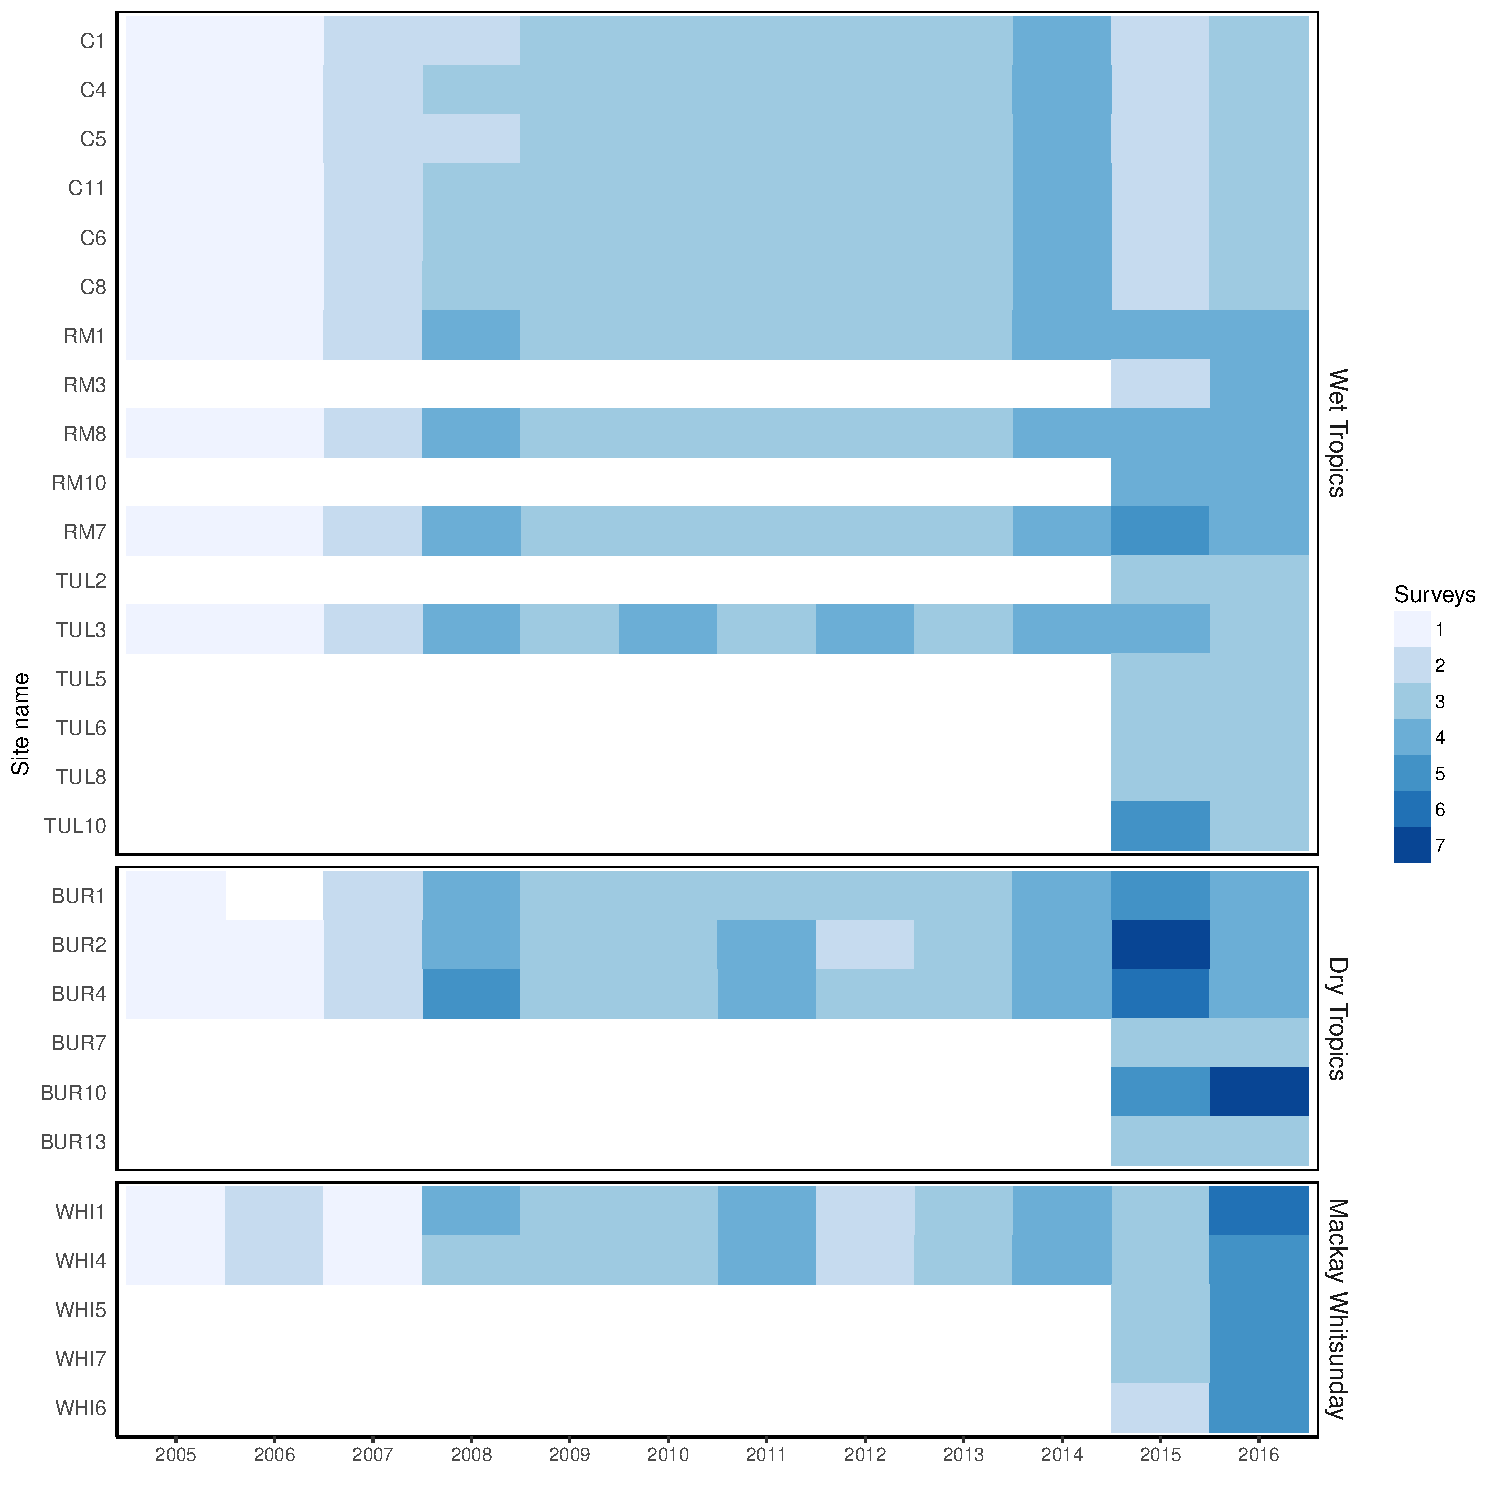
\includegraphics[width=1\linewidth]{figures/Maps/Insitu_sites/Samples_spatial_temporal.pdf}
\caption{Spatial and temporal distribution of AIMS insitu samples.  Sites names follow Great Barrier
Reef Marine Park Authority (GBRMPA) and sites are arranged north to south into the focal
Regions. Blue shading of tiles denotes the number of surveys conducted in the year at each
site.}\label{fig:AIMS_insitu_spatial_temporal}
\end{figure}
 
  \arrayrulecolor[rgb]{0.06,0.25,0.49}
 \LTcapwidth=\linewidth
 \setlength\aboverulesep{0pt}\setlength\belowrulesep{0pt}
 \setlength\cmidrulekern{1pt}\setlength\cmidrulewidth{1pt}
 \renewcommand\arraystretch{1.2}\setlength\tabcolsep{5pt}
 \begin{table}\caption{Measures collected in AIMS MMP insitu inshore water quality monitoring program.  NOx is the sum of NO$_2$ and NO$_3$.  Data used are annual means of depth weighted averages per site.}\label{tab:insitu.measures}
 %\begin{center}
 \scriptsize
 \begin{tabular}{
 !{\color[rgb]{0.06,0.25,0.49}\VRule[1pt]} p{10em}
 !{\color[rgb]{0.06,0.25,0.49}\vline} l
 !{\color[rgb]{0.06,0.25,0.49}\vline} p{15em}
 !{\color[rgb]{0.06,0.25,0.49}\vline} l
 !{\color[rgb]{0.06,0.25,0.49}\vline} l
 !{\color[rgb]{0.06,0.25,0.49}\vline} l
 !{\color[rgb]{0.06,0.25,0.49}\VRule[1pt]}
 }
 \arrayrulecolor[rgb]{0.06,0.25,0.49}\specialrule{1pt}{0pt}{0pt} %top border
 \rowcolor[rgb]{0.53,0.62,0.74} 
 \multicolumn{1}{!{\color[rgb]{0.06,0.25,0.49}\VRule[1pt]}l}{\whiteHeader{{Measure}}} & 
 \multicolumn{1}{l}{\whiteHeader{{Variable}}} & 
 \multicolumn{1}{l}{\whiteHeader{{Description}}} & 
 \multicolumn{1}{l}{\whiteHeader{{Abbreviation}}} & 
 \multicolumn{1}{l}{\whiteHeader{{Conversion}}} & 
 \whiteHeader{{Units}}\\ 
 \cmidrule{1-6} 
Chlorophyll-a & DRIFTCHL\_UGPERL.wm & Chlorophyll-a (µg/L) & chl & x1 & µgL^{-1} \\ 
   \cline{1-6}Total Suspended Solids & TSS\_MGPERL.wm & Suspended solids (mg/L) & nap & x1 & mgL^{-1} \\ 
   \cline{1-6}Secchi Depth & SECCHI\_DEPTH.wm & Secchi depth (m) & sd & x1 & m \\ 
   \cline{1-6}NOx & NOX.wm & Nitrite and Nitrate measured by microanalyser (µM/L) & NOx & x14 & µgL^{-1} \\ 
   \bottomrule
 \end{tabular}
 %\end{center}
 \end{table}


\clearpage

\subsection{AIMS FLNTU samples}
  
Combination continuous Flourometer and Turbidity Sensors (hereafter FLNTU) loggers were deployed at
15 of the AIMS MMP inshore water quality monitoring sites.
 
  \arrayrulecolor[rgb]{0.06,0.25,0.49}
 \LTcapwidth=\linewidth
 \setlength\aboverulesep{0pt}\setlength\belowrulesep{0pt}
 \setlength\cmidrulekern{1pt}\setlength\cmidrulewidth{1pt}
 \renewcommand\arraystretch{1.2}\setlength\tabcolsep{5pt}
 \begin{table}[h]\caption{Measures collected in AIMS MMP flntu inshore water quality monitoring program. Data used are daily means per site.}\label{tab:flntu.measures}
 %\begin{center}
 \scriptsize
 \begin{tabular}{
 !{\color[rgb]{0.06,0.25,0.49}\VRule[1pt]} p{10em}
 !{\color[rgb]{0.06,0.25,0.49}\vline} l
 !{\color[rgb]{0.06,0.25,0.49}\vline} p{15em}
 !{\color[rgb]{0.06,0.25,0.49}\vline} l
 !{\color[rgb]{0.06,0.25,0.49}\vline} l
 !{\color[rgb]{0.06,0.25,0.49}\vline} l
 !{\color[rgb]{0.06,0.25,0.49}\VRule[1pt]}
 }
 \arrayrulecolor[rgb]{0.06,0.25,0.49}\specialrule{1pt}{0pt}{0pt} %top border
 \rowcolor[rgb]{0.53,0.62,0.74} 
 \multicolumn{1}{!{\color[rgb]{0.06,0.25,0.49}\VRule[1pt]}l}{\whiteHeader{{Measure}}} & 
 \multicolumn{1}{l}{\whiteHeader{{Variable}}} & 
 \multicolumn{1}{l}{\whiteHeader{{Description}}} & 
 \multicolumn{1}{l}{\whiteHeader{{Abbreviation}}} & 
 \multicolumn{1}{l}{\whiteHeader{{Conversion}}} & 
 \whiteHeader{{Units}}\\ 
 \cmidrule{1-6} 
Chlorophyll-a & CHL\_QA\_AVG & ?? & chl & CHL\_QA\_AVG x1 & µgL^{-1} \\ 
   \cline{1-6}NTU & NTU\_QA\_AVG & ?? & ntu & NTU\_QA\_AVG x1 & NTU \\ 
   \bottomrule
 \end{tabular}
 %\end{center}
 \end{table}
 

\begin{figure}[ptbh] \includegraphics[width=1\linewidth]{figures/Exploratory_Data_Analysis/FLNTU/flntu_temporal\res.pdf}
\caption{Spatial and temporal distribution of AIMS FLNTU samples (Red: NTU, Green: Chlorophyll-a).
Sites names follow Great Barrier Reef Marine Park Authority (GBRMPA) and sites are arranged north to
south into the focal Regions.}\label{fig:flntu_temporal}
\end{figure}

\clearpage

\subsection{Remote sensing (BOM satellite)}

Daily (July 2002--Dec 2016, $1\times 1 km^2$ resolution) Moderate Resolution Imaging
Spectroradiometer (MODIS satellite) imagery (hereafter referred to as Satellite) data were obtained
by downloading NETCDF files from the thredds server (http://ereeftds.bom.gov.au/ereefs/tds/catalog/ereef/mwq/P1D/2002/catalog.html).
The data referred to herein relates to the individual measures considered in the data exploration
component of the project, and is distinct from the surface reflectance data used in the eReefs data
assimilation scheme discussed below in section \ref{sec:eReefs}.

  \arrayrulecolor[rgb]{0.06,0.25,0.49}
 \LTcapwidth=\linewidth
 \setlength\aboverulesep{0pt}\setlength\belowrulesep{0pt}
 \setlength\cmidrulekern{1pt}\setlength\cmidrulewidth{1pt}
 \renewcommand\arraystretch{1.2}\setlength\tabcolsep{5pt}
 \begin{table}[h]\caption{Measures collected from MODIS satellite imaging. Data used are daily means per pixel. Variable and Description pertain to the eReefs source.  Conversion indicates the conversion applied on data to conform to threshold Units.  Abbreviation provides a consistent key accross data. MIM refers to the robust and scalable matrix inversion method used to handle the variability in optical properties of satellite imagery.}\label{tab:satellite.measures}
 %\begin{center}
 \scriptsize
 \begin{tabular}{
 !{\color[rgb]{0.06,0.25,0.49}\VRule[1pt]} p{10em}
 !{\color[rgb]{0.06,0.25,0.49}\vline} l
 !{\color[rgb]{0.06,0.25,0.49}\vline} p{20em}
 !{\color[rgb]{0.06,0.25,0.49}\vline} l
 !{\color[rgb]{0.06,0.25,0.49}\vline} l
 !{\color[rgb]{0.06,0.25,0.49}\vline} l
 !{\color[rgb]{0.06,0.25,0.49}\VRule[1pt]}
 }
 \arrayrulecolor[rgb]{0.06,0.25,0.49}\specialrule{1pt}{0pt}{0pt} %top border
 \rowcolor[rgb]{0.53,0.62,0.74} 
 \multicolumn{1}{!{\color[rgb]{0.06,0.25,0.49}\VRule[1pt]}l}{\whiteHeader{{Measure}}} & 
 \multicolumn{1}{l}{\whiteHeader{{Variable}}} & 
 \multicolumn{1}{l}{\whiteHeader{{Description}}} & 
 \multicolumn{1}{l}{\whiteHeader{{Abbreviation}}} & 
 \multicolumn{1}{l}{\whiteHeader{{Conversion}}} & 
 \whiteHeader{{Units}}\\ 
 \cmidrule{1-6} 
Chlorophyll-a & Chl\_MIM} & Near surface concentration based on empirical relationship established between in situ measurements and blue-to-green band ratios & chl & Chl\_MIM} x1 & µgL^{-1} \\ 
   \cline{1-6}Non-Algal Particles & Nap\_MIM} & Total suspended solids based on relationship established between in situ measurements and the absorption concentration of non-algal particles & nap & Nap\_MIM} x1 & mgL^{-1} \\ 
   \cline{1-6}Secchi Depth & SD\_MIM} & Secchi depth based on empirical relationship established between in situ measurements and estimated depth at which 10\% of surface light still available & sd & SD\_MIM} x1 & m \\ 
   \bottomrule
 \end{tabular}
 %\end{center}
 \end{table}


 

%\subsection{eReefs assimilated model}

\subsection[eReefs coupled hydrodynamic]{eReefs coupled hydrodynamic - biogeochemical model}\label{sec:eReefs}

\begin{itemize}
\item \textcolor{red}{We need a table that specifies and explains the naming of the various
    eReefs models and where they are available}
\end{itemize}

The eReefs coupled hydrodynamic, sediment and BGC modelling system involves the application of a
range of physical, chemical and biological process descriptions to quantify the rate of change of
physical and biological variables (Fig.~\ref{fig:bgc}, \citet{Schiller14}). The processes
descriptions are generally based either on a fundamental understanding of the process (such as the
effect of gravity on circulation) or measurements when the process is isolated (such as the maximum
division rate of phytoplankton cells at 25$^{\circ}$C in a laboratory mono-culture). The model also
requires as inputs external forcings, such as observed river flows and pollutant loads. Thus, the
model can be run without observations from the marine environment and in this mode is quite skilful
(\citet{Skerratt18} and below). This mode which does not use observations from the marine
environment as the simulation is undertaken is referred to as the non-assimilating simulation. Most
of the eReefs marine biogeochemical simulations are non-assimilating.

\begin{figure}[thb]
\begin{center}
\resizebox{5in}{!}{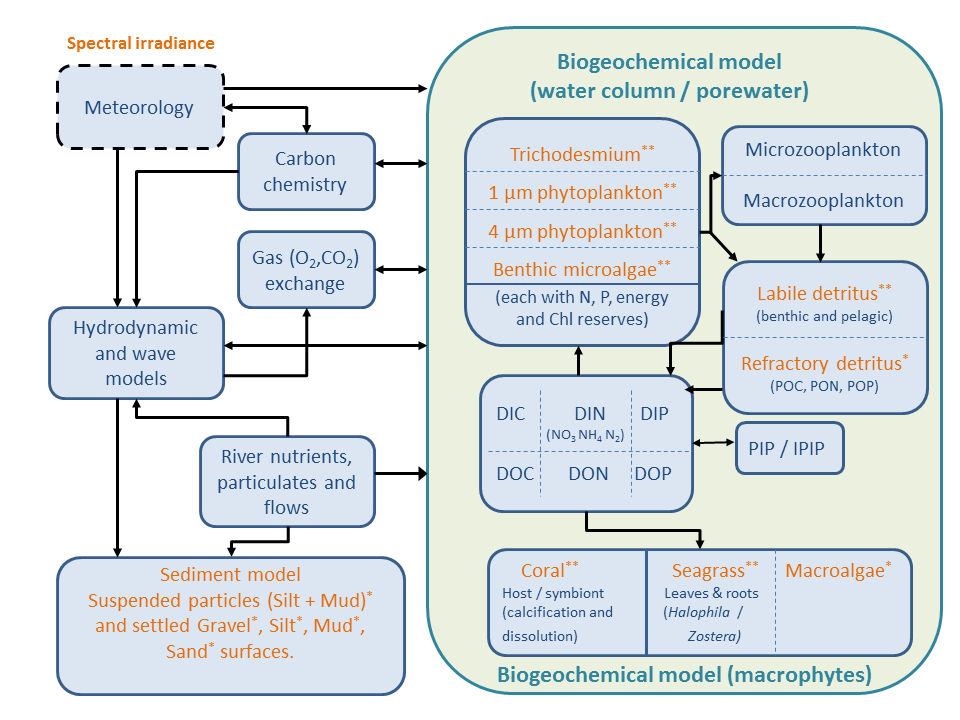
\includegraphics{figures/Mark/ereefsbgcdiagram4emlyn.png}}
\caption{Schematic showing eReefs coupled hydrodynamic biogeochemical model.}
\label{fig:bgc}
\end{center}
\end{figure}

\begin{figure}[thb]
\begin{center} \resizebox{5in}{!}{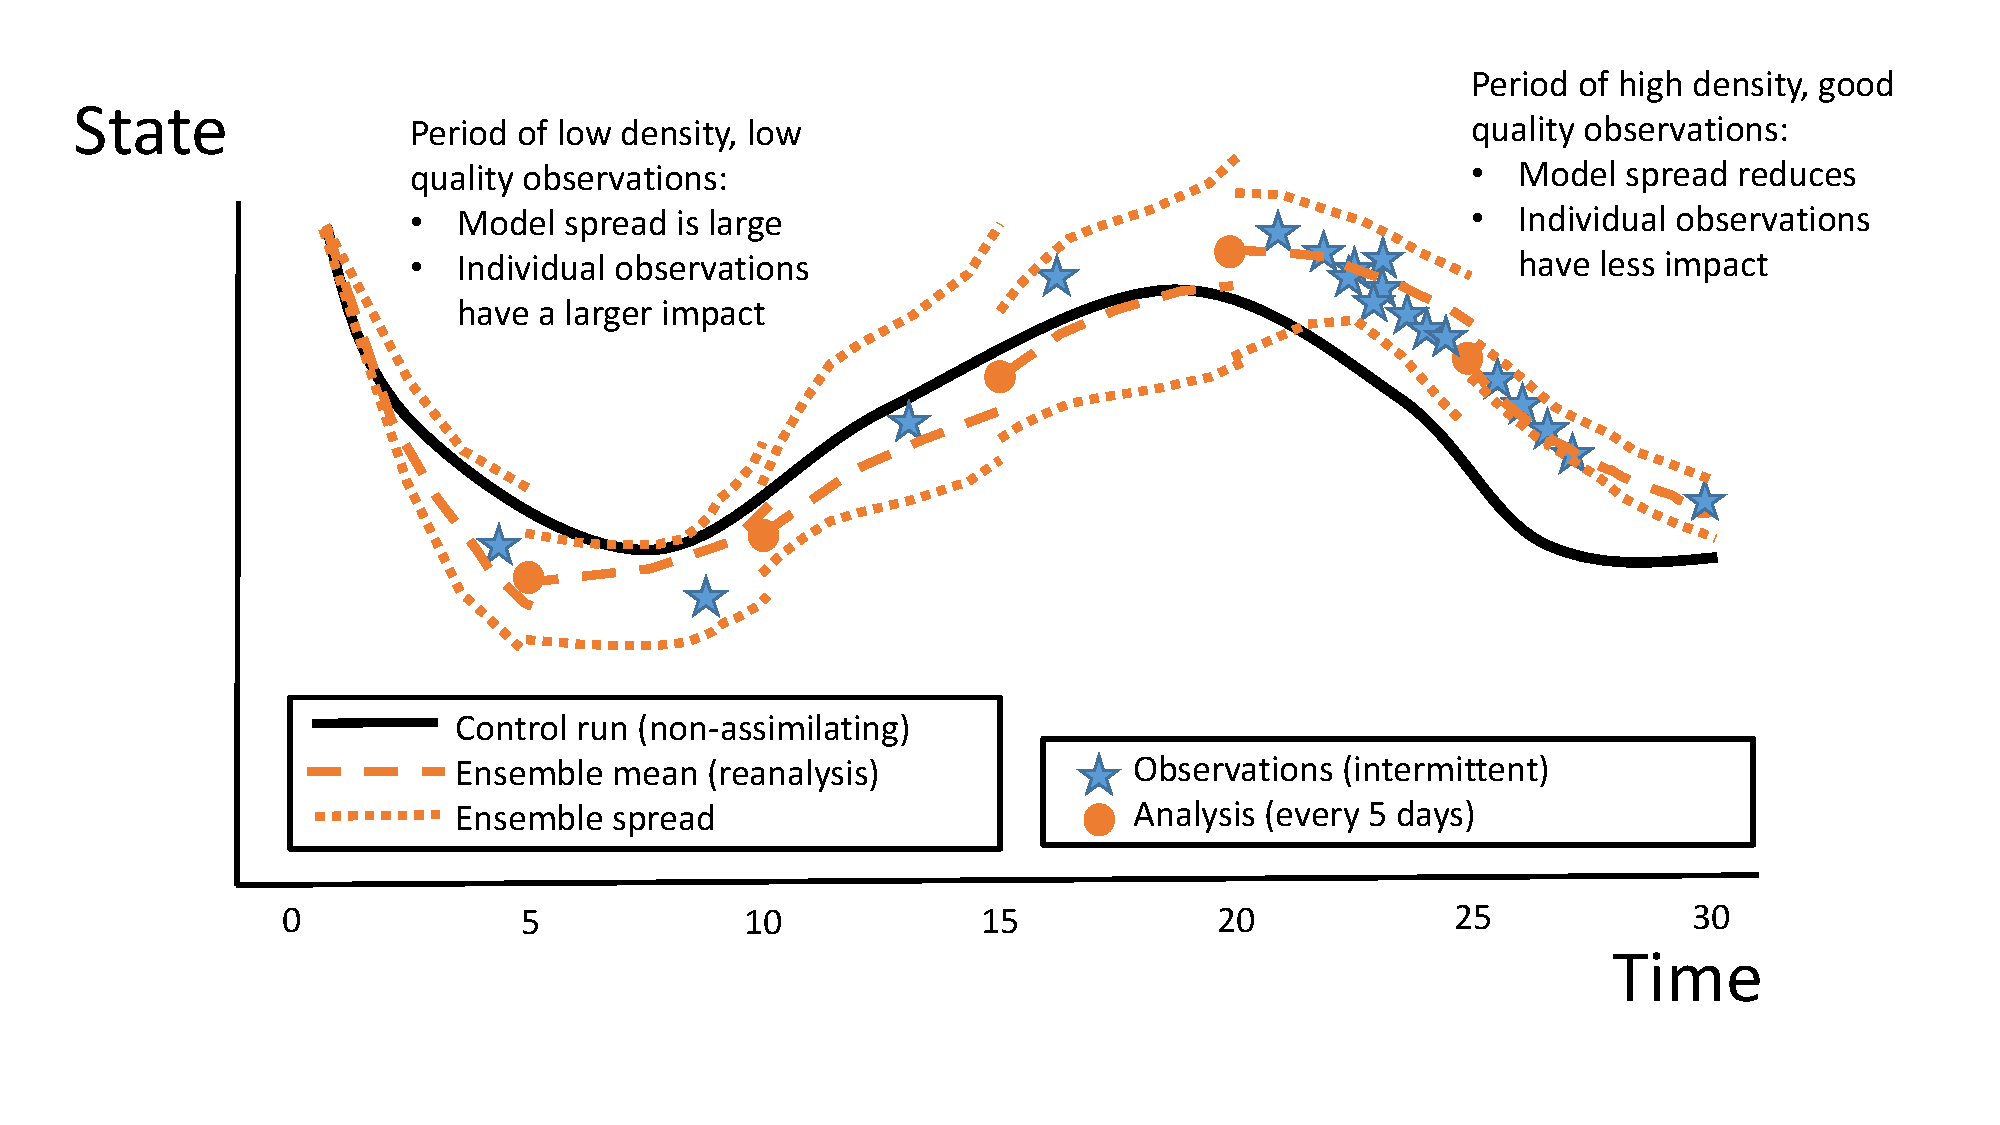
\includegraphics{figures/Mark/EnKFschematic.pdf}}
\caption{Schematic showing the evolution of the model ensemble over 6 assimilation cycles using the
Ensemble Karman Filter (EnKF) system. The non-assimilating control run (black line) is capturing the
gross cycle in the observations (blue stars), but errors remain that observations can constrain. At
the initial time, all ensemble members, and the control run, have similar values.  In the first five
days the 108 members develop a spread, with the control run being different to the ensemble mean,
but within the ensemble spread. At 5 days, the first state updating occurs. In the first 5 days
there was only one observations, being above the ensemble mean. At day 5, a new state for the entire
ensemble is calculated (the analysis being the mean of the updated ensemble) based on the mismatch
between the ensemble members and observations. The updated state is closer to the model if the
ensemble spread is small, or to the observations if they are dense with few errors. At day 5,
because of the small positive mismatch, the ensemble spread is only slightly narrowed, and the mean
increased. The ensemble members all restart from these new updated states. The next four analysis
steps proceed much like the first. For the fifth analysis step, high density observation were
available over the previous 5 days, so the analysis is weighted heavily toward the observations, and
the model spread is constrained significantly. Looking at the error between the ensemble mean and
the observations over the entire period we see that the data assimilation system has provided an
improved estimate of the state (the mean of the ensemble) relative to the control run, and achieved
this using the model that contains the processes we understanding to describe system.}
\label{fig:da}
\end{center}
\end{figure}

Despite being already skilful, the predictive skill of the model can be improved by assimilating
marine observations into an ensemble (i.e. a large number (108) of similar but not identical) of
model simulations. The form of data assimilation we chose, and that is commonly used in weather
forecasting, involves updating of the state of the model as the simulation progresses
(Fig.~\ref{fig:da}). State updating involves first looking for a mismatch between the state of the
ensemble members and the observations over the previous 5 days. Ocean colour, the observation of
water-leaving irradiance at 8 individual wavebands, provides the only data set with sufficient
temporal (daily) and spatial (1 km) resolution, providing upwards of 13 million pixels on a
cloud-free day. For this comparison, we have chosen to use the mismatch between the model's
prediction of the ratio of the water-leaving irradiance at 443 nm (blue) and 551 nm (green) and the
observation of the same quantities from the MODIS sensor on NASA's Aqua satellite. The eReefs
biogeochemical model is the first published model to assimilate raw ocean colour observations
\citep{Jones16}. The data assimilation algorithm uses the model-observation mismatch, as well as
statistically-quantified dynamical properties of model, to periodically alter the values in the 108
member ensemble, resulting the ensemble mean gaining a closer match to the observations. The outcome
of this modelling system is referred to in the field of data assimilation as a reanalysis.

Below we describe the model itself, and then particular data assimilation system.

\subsubsection{eReefs coupled model description and forcing}

The hydrodynamic model is a fully 3-D finite-difference baroclinic model based on the 3-D equations
of momentum, continuity and conservation of heat and salt, employing the hydrostatic and Boussinesq
assumptions \citep{Herzfeld06,Herzfeld15a}. The sediment transport model adds a multilayer sediment
bed to the hydrodynamic model grid and simulates sinking, deposition and resuspension of multiple
size classes of suspended sediment \citep{Margvelashvili09,Margvelashvili16}. The complex BGC model
simulates optical, nutrient, plankton, benthic organisms (seagrass, macroalgae and coral), detritus,
chemical and sediment dynamics across the whole GBR region, spanning estuarine systems to
oligotrophic offshore reefs (Fig.~\ref{fig:bgc}, \citet{Baird16a}). An expanded description of the
BGC model is given in Appendix A, with a brief description of the optical model in Appendix
B. Briefly, the BGC model considers four groups of microalgae (small and large phytoplankton,
Trichodesmium and microphytobenthos), two zooplankton groups, three macrophytes types (seagrass
types corresponding to Zostera and Halophila, macroalgae) and coral communities.

Photosynthetic growth is determined by concentrations of dissolved nutrients (nitrogen and
phosphorous) and photosynthetically active radiation. Microalgae contain two pigments (chlorophyll a
and an accessory pigment) and have variable carbon : pigment ratios determined using a
photoadaptation model (described in \citet{Baird13}. Overall, the model contains 23 optically active
constituents (\citet{Baird16a}; and Appendix A).

The model is forced with freshwater inputs at 21 rivers along the GBR and the Fly River in southwest
Papua New Guinea. River flows are obtained from the DERM (Department of Environment and Resource
Management) gauging network. Nutrient concentrations flowing in from the ocean boundaries were
obtained from the CSIRO Atlas of Regional Seas (CARS) 2009 climatology \citep{Ridgway02}.

The nutrient loads (TSS, PN, PP, DIN,DIP) for the 21 rivers were obtained from the process-based
Source models used for Paddock 2 Reef (P2R) load reduction estimates \citep{Waters14}. The P2R
represenst land uses and landscape processes in a variety of ways, often based upon spatially
explicit farm-scale models that are included through a system of bespoke pre-processing and transfer
tools. These P2R Source models also include flow related in-stream processing of pollutants, thus
altering loads as fluxes transfer throughout the network. P2R modelling includes scenarios designed
to represent ‘baseline’ (or ‘current condition’) and ‘pre-development’ catchment loads. In this
report we only use 'baseline' condition. The reliance of the base P2R Source models on external,
farm scale sub-models, means that they cannot be easily modified to extend the period covered by the
report card. Thus we only use the P2R outputs from Jan 2011 - July 2014.

In order to provide daily timeseries predictions of pollutant loads past July 2014, the reliance on
external sub-models was replaced by pollutant generation models that estimate daily loads through
monthly varying concentrations (‘EMC/DWC’). The particular concentration values for each pollutant
for each Functional Unit (FU) within each subcatchment have been calculated by analysing the monthly
runoff volumes and pollutant loads from the P2R Source models defined in \citet{Waters14}. The
network transport and in-stream processing mechanisms are unaltered from the base P2R Source
models. These monthly concentration pollutant generation models allow the model predictions to be
extended by providing updated rainfall runoff model inputs (i.e. the runoff of the day), without the
need to also update many thousands of farm scale sub-models. Simple comparisons of predicted loads
indicates that the monthly varying concentration approach works reasonably well for sediment and
associated particulate nutrient, and less well for pollutants that are usually reliant on farm scale
representation of management inputs.

\subsubsection{Assimilation system}

%\subsubsection{Assimilation of ocean colour}
\paragraph{Assimilation of ocean colour}

Ocean colour was chosen as the data set to assimilate due to its availability over the entire GBR at
high temporal and spatial density. Ocean colour has often been used for biogeochemical data
assimilation \citep{Kidston13}. In global biogeochemical data assimilation applications, the
observation - model mismatch used has often been satellite estimates of \textit{in situ} chlorophyll
concentration versus model predicted chlorophyll concentration \citep{Ford12}. This approach is
problematic in coastal waters such as the GBR, where chlorophyll concentration is often
overestimated by satellite algorithms due to bottom reflectance or absorption by non-phytoplankton
components \citep{Schroeder12b}. So it is not possible in this application to base the data
assimilation system on the mismatch of model chlorophyll against satellite estimates of \textit{in
situ} chlorophyll. Instead, we have pioneered the use of remote-sensing reflectance as the variable
to determine the mismatch between the observed and modelled quantities \citep{Jones16}.

Remote-sensing reflectance, $R_{rs}$, is the ratio of the water-leaving irradiance in the direction
of a satellite to the water entering radiance. In this sense it is a 'raw' satellite
observation. The value of $R_{rs}$ varies with wavelength and is measured in sr$^{-1}$ (sr =
steradians, the SI unit of solid angle, where the solid angle in all direction on a spherical
surface is $4 \pi$ sr). In the open ocean at blue wavelengths the value is around 0.03 sr$^{-1}$
\citep{Baird16a}. That is, 3 \% of the light that entered the ocean within 1 m$^{2}$ emerged
travelling in the direction within a solid angle of 1 sr (i.e. $1 / 4 \pi$ of a sphere).

The model contains 23 optically active constituents (shaded orange in Fig.~\ref{fig:bgc}, see also
\citet{Baird16a}). For each of these constituents the optical model calculates the rate of
absorption, scattering and backscattering. To calculate $R_{rs}$ at the surface, we need to consider
the light returning from multiple depths, and from the bottom. Rather than using a computationally
expensive radiative transfer model, we approximate $R_{rs}$ based on an optical-depth weighted
scheme \citep{Baird16a}. The model sums the return from each depth (and the bottom) to give the
surface $R_{rs}$. As shown in \citet{Baird16a}, this calculation is sufficiently accurate that the
primary reason for the mismatch between observed and modelled $R_{rs}$ is errors in the coupled
hydrodynamic-biogeochemical model prediction of optically-active constituents. This is, of course,
the result we wanted - it means that when the assimilation system updates the optically-active
biogeochemical constituents in order to minimise the mismatch between observed and modelled
$R_{rs}$, it is changing the components of the model that have the greatest errors, and in doing so
improving the solution of those parts that we most care about - the optically-active components that
determine water clarity.

When testing the data assimilation system, we found that the best quantity to assimilate was the
ratio of the remote-sensing reflectance at 443 and 551 nm. In fact, this ratio is the same one used
in the NASA OC3M algorithm that we mentioned above is NOT a good measure of \textit{in situ}
chlorophyll in coastal waters! So how can it be that OC3M is a poor predictor of \textit{in situ}
chlorophyll in coastal waters, yet assimilating the mismatch between simulated OC3M and
satellite-observed OC3M achieves the best skill for \textit{in situ} chlorophyll when compared
against independent \textit{in situ} observations? The answer lies in that simulated OC3M is
calculated using the ratio of two simulated $R_{rs}$, in the same manner in which observed OC3M is
calculated using the ratio of two observed $R_{rs}$. Fig.~\ref{fig:OC3M} shows the \textit{in situ}
chlorophyll concentration, the simulated OC3M and the NASA observed OC3M for the Cape York region on
a relatively clear day.  The \textit{in situ} chlorophyll concentration in coastal regions along
this coast is $\sim 0.5$ mg m$^{-3}$ (Fig.~\ref{fig:OC3M} left). The simulated OC3M, calculated from
simulated $R_{rs}$, is greater along the coastal fringe due to the absorption of blue light from
CDOM, and addition bottom reflection of green light (Fig.~\ref{fig:OC3M} centre). The observed OC3M,
also affected by CDOM absorption and the bottom, looks more like the simulated OC3M than the
\textit{in situ} chlorophyll concentration (Fig.~\ref{fig:OC3M} right). Further, where there are
differences, the primary cause is the error in the simulated water-column optically-active
constituents like chlorophyll. Thus by producing the same simulated and observed quantity, we have
improved the ability of the assimilation system to update the optically-active model constituent
that is in error.

\begin{figure}[thb]
\begin{center} \resizebox{5in}{!}{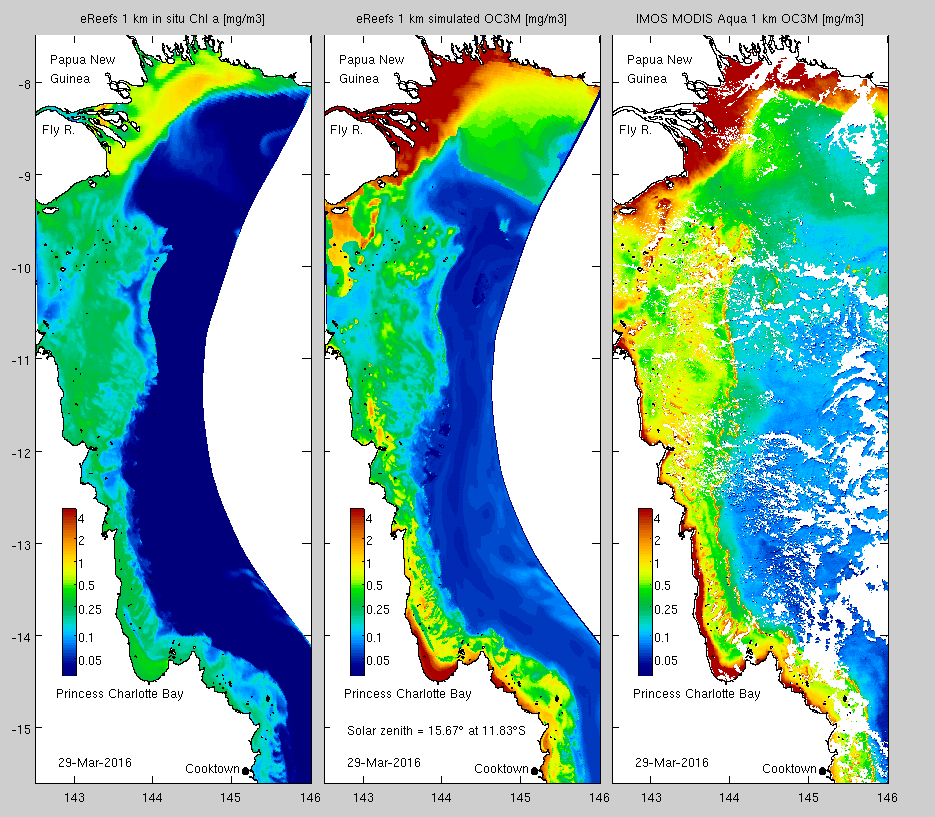
\includegraphics{figures/Mark/OC3M4reanalysis.png}}
\caption{Example of the estimates of OC3M in the Cape York region on the 29 March 2016 using the 1
km GBR1 model and the NASA Aqua MODIS sensor: \textit{in situ} chlorophyll concentration (left), the
simulated OC3M (centre) and the NASA observed OC3M (right).}
\label{fig:OC3M}
\end{center}
\end{figure}

OC3M uses the ratio of above-surface remote-sensing reflectance as a combination of three
wavelengths, $R'$, which is given by:
\begin{equation} R' = \log_{10} \left( \mathrm{max} \left[ R_{rs,443}, R_{rs,488} \right] /
R_{rs,551} \right)
\end{equation} The ratio $R'$ is used in the OC3M algorithm to estimate surface chlorophyll,
$\mathrm{Chl}_{OC3}$, with coefficients from the 18 March 2010 reprocessing:
\begin{equation} \mathrm{Chl}_{OC3} = 10^{0.283 + R' \left(-2.753 + R' \left( 1.457 + R' \left(0.659
- 1.403 R' \right) \right) \right)}
\end{equation} obtained from \texttt{oceancolor.gsfc.nasa.gov/REPROCESSING/R2009/ocv6/}. Using, OC3M
we gain the benefit of assimilating directly the mismatch between the simulated OC3M (based on
simulated remote-sensing reflectance) and the observed remote-sensing reflectance; and we use a
quantity that has meaning in the water quality community (mass concentration of chlorophyll). To
re-state, because we use the simulated remote-sensing reflectance to calculate OC3M, the system is
not affected by the inaccuracies in the relationship between in situ chlorophyll and
satellite-derived OC3M. And our assimilation system's prediction of chlorophyll is the simulated
\textit{in situ} chlorophyll concentration (and not OC3M).

The accuracy of the modelling systems also requires that the model and observations are closely
matched in space and time. This is because remote-sensing reflectance is a function of solar angle
(and therefore time of day), and because the optical properties of coastal waters can vary quickly
due to a range of processes such as phytoplankton chlorophyll synthesis, movement of fronts, wind
driven-upwelling, river plume structure changes etc. We used the flexible outputting time of the
model, and the asynchronous assimilation routines in the EnKF-C package \citep{Sakov17}, to closely
align the observations and models. In doing so we were able to meet the $\pm 30$ minutes matching
requirements used for the calibration / validation of ocean colour satellite products.

The Aqua satellite overpasses the GBR between 1130 and 1530 locally. In order to match the model
output to within 30 minutes of the overpass, the model remote-sensing reflectance was output at
1200, 1300, 1400 and 1500 daily. For the calculations of remote-sensing reflectance, the water
column calculations of the light field (and $R_{rs}$) was redone on the output time assuming the
entire grid is at 150$^{\circ}$E, while infact it varies from 142$^{\circ}$31'E to
156$^{\circ}$51'E. Thus the maximum error in calculating solar angle for the purposes of outputting
$R_{rs}$, in the Torres Strait, is about 30 minutes (this small error will be corrected in the next
phase of eReefs). The light field calculation was also done at wavelengths at the centre of the
MODIS ocean colour bands to avoid any small interpolations from the spectrally-resolved model that
has a 20 nm resolution.

The observations also need to be spatially aligned. The observations are at approximately $\sim$1 km
resolution (up to 2 km on the edges of the swath), with location varying spatially with each
different satellite swath. Meanwhile the model cells are stationary, are $\sim$ 16 km$^2$, and are
defined on the curvilinear grid. The observations are grouped into a "superobservation" for each
model cell. The superobservation contains all observations that were closer to a particular cell
centre than any other cell centre. The position of the superobservation is the mean of the
observations it is composed of, and will be close to, but not exactly the same, as the location of
the cell centre. The assimilation system then accounts for the now small misalignment in time and
space when considering the mismatch between the model and observation.

%\subsubsection{Ensemble member design}
\paragraph{Ensemble member design}

The assimilation system used in this study is the Determininstic Ensemble Kalman Filter (DEnKF) that
requires an ensemble of model runs that approximate the uncertainty in the model solution.  The
uncertainty in the model solution arises from uncertainty in the model initial conditions, boundary
conditions, surface forcing and model parameterisations.  The ensemble members differ in the values
of the quadratic mortality rate coefficient of small zooplankton, in the loads of nutrients
delivered in the rivers (as a multiple of the SOURCE catchments specified loads), and in the PAR
light forcing (again as a multiple of the Bureau of Meteorology short wave radiation
prediction). These relatively small differences, which are undertaken on the most uncertain
biological parameter, and most sensitive forcing paramaters, provide a spread of ensemble members
that the Karman Filter can operate on.

For a further description of the numerical schemes in the assimilation system see \citep{Jones16}. A
number of modifications have been made to improve the accuracy and efficiency of the system,
including transferring the the EnKF-C software.

\subsubsection{Summary results}

The non-assimilating version of the model has been compared to observations previously (ereefs.info,
\citet{Baird16a} and \citet{Skerratt18}). The results produced in the reanalysis are compared
directly to observations in the attached 100 page appendix showing comparisons to hundreds of
time-series. Further, later components of this document compare the metric calculated using the
non-assimilating model, the assimilating model, satellite observations and \textit{in situ}
observations. Here we will just show a few snapshot results to aid in the understanding of the
performance of the data assimilation relative to the non-assimilating run.

%\subsubsection{Assessment of chlorophyll concentration at MMP sites}
\paragraph{Assessment of chlorophyll concentration at MMP sites}

In our assessment of the skill of the eReefs biogeochemical models, we have considered the most
important property to be the prediction of \textit{in situ} chlorophyll concentration at the MMP
sites. For this there are two measures - the chlorophyll extractions at the sampling sites, and the
calibrated chlorophyll fluorescence on the moorings.  While the extractions are considered the most
accurate, the fluorescence time-series is continuous. When the two are lined up in time (they are
slightly separated in space), the mismatch between the observed chlorophyll extractions and the
observed chlorophyll fluorescence is 0.2 mg m$^{-3}$. We use this 0.2 mg m$^{-3}$ as indicative of
the error of the observations.

It is important to note that the \textit{in situ} chlorophyll concentration observations were not
assimilated into the model. That is, they were observation withheld just for the model
assessment. In fact, the mismatch between observed and modelled quantities used in the assimilation
system is neither an \textit{in situ} measurement, nor a chlorophyll concentration. The assimilated
quantity was the ratio of remote-sensing reflectance at blue and green wavelengths. Thus, we can be
confident that if the assimilation system has improved the prediction of \textit{in situ}
chlorophyll concentration then it has improved the overall biogeochemical model.

At 13 of the 14 MMP site, the assimilation of satellite-observed remote-sensing reflectance improved
the prediction \textit{in situ} chlorophyll concentration (Fig.~\ref{fig:RMSerror}, top). On average
the assimilation reduced the error from 0.34 to 0.29 mg m$^{-3}$, bring it 30 \% closer to the
observation error (the limit of our ability to quantify an improvement in the model). The worst two
site remained the most coastal sites, Geoffrey Bay and Dunk Island, for which the 4 km model poorly
resolves local processes, and for which the assimilation system would provide little information to
water column due to the optically-shallow and complex waters. The best site was Double Cone Island
off Airlie Beach. At Double Cone Island, a time-series shows the improvement in the chlorophyll
fluorescence due to the assimilation (Fig.~\ref{fig:RMSerror}, bottom). During a particularly
cloud-free period in the second half of 2015, the assimilation system does a remarkable job of both
removing model bias and capturing variability in the model.


\begin{figure}[thb]
\begin{center} \resizebox{5in}{!}{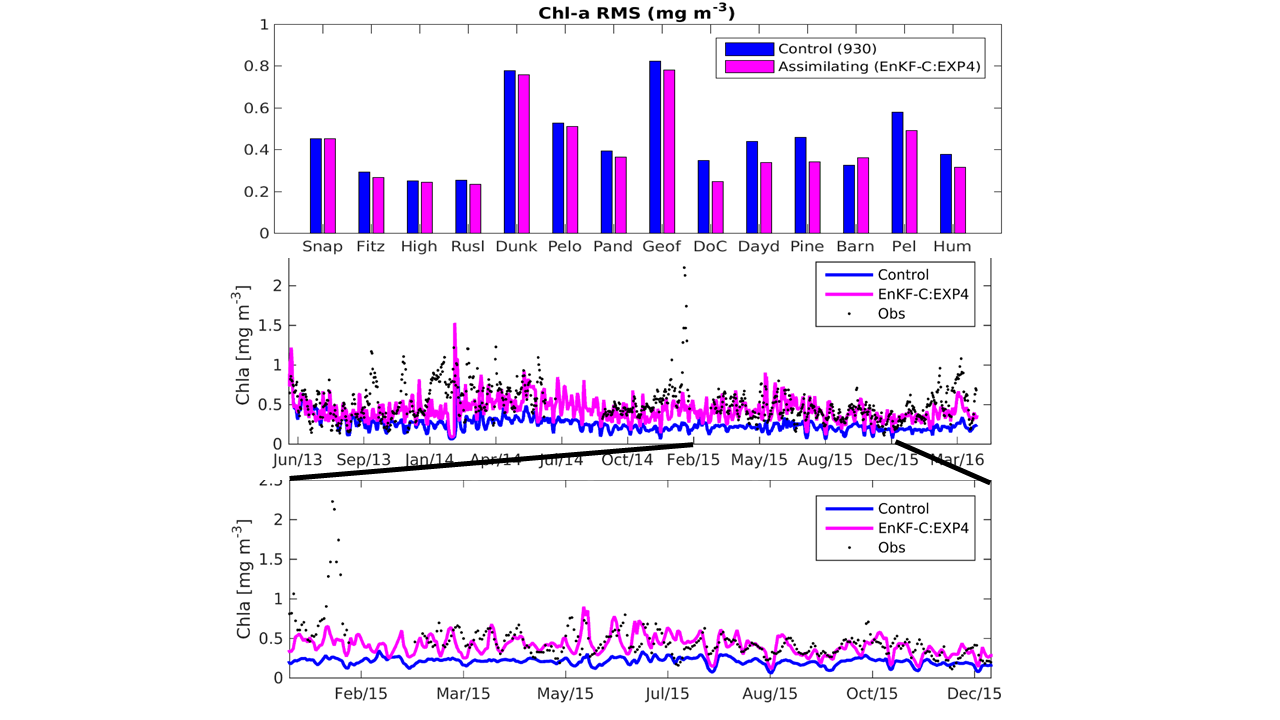
\includegraphics{figures/Mark/reanalysisRMSerror.png}}
\caption{Comparison of the non-assimilating (blue) and assimilating (pink) runs at the MMP
sites. The instantaneous state root mean square error at the 14 MMP sites (top). The approximate
error in the observations is 0.2 mg m$^{-3}$. At Double Cone Island in the Whitsundays (off Airlie
Beach), a time-series of the observations (black dots) and simulations is shown for the whole
simulations (centre) and the a 1 year period (bottom).}
\label{fig:RMSerror}
\end{center}
\end{figure}


% **Mark to provide a brief description**.

\arrayrulecolor[rgb]{0.06,0.25,0.49}
\LTcapwidth=\linewidth
\setlength\aboverulesep{0pt}\setlength\belowrulesep{0pt}
\setlength\cmidrulekern{1pt}\setlength\cmidrulewidth{1pt}
\renewcommand\arraystretch{1.2}\setlength\tabcolsep{5pt}
\begin{table}[ht]\caption{eReefs regional biogeochemical simulation catalog.}\label{tab:ereefs}
  \scriptsize
  \begin{tabular}{
    !{\color[rgb]{0.06,0.25,0.49}\VRule[1pt]} p{15em}
    !{\color[rgb]{0.06,0.25,0.49}\vline}l
    !{\color[rgb]{0.06,0.25,0.49}\vline}l
    !{\color[rgb]{0.06,0.25,0.49}\vline}l
    !{\color[rgb]{0.06,0.25,0.49}\vline}l
    !{\color[rgb]{0.06,0.25,0.49}\vline}l
    !{\color[rgb]{0.06,0.25,0.49}\VRule[1pt]}
    }
    \arrayrulecolor[rgb]{0.06,0.25,0.49}\specialrule{1pt}{0pt}{0pt} %top border
    \rowcolor[rgb]{0.53,0.62,0.74}
    \multicolumn{1}{!{\color[rgb]{0.06,0.25,0.49}\VRule[1pt]} p{15em}}{\whiteHeader{{Simulation name}}} & 
    \multicolumn{1}{l}{\whiteHeader{{Projects}}}&
    \multicolumn{1}{l}{\whiteHeader{{Date range}}}&
                                                    \multicolumn{1}{l}{\whiteHeader{{Delivery}}}&
                                                                                                  \whiteHeader{{Notes/Improvements}}\\
    \cmidrule{1-5}
    GBR4\_H1p85\_B1p0\_Cbas\_Dhnd & SIEF & Jan 1, 2011 -- Jun 30, 2014 & Available on NCI & Simulation delivered as part of SIEF project (previously known as 926). Skill assessment available in SIEF report.\\
    \cline{1-5}& & & &\\
    \cline{1-5}& & & &\\
    \bottomrule
  \end{tabular}
\end{table}


In this context, the \textbf{eReefs} model refers to the
GBR4\_H2p0\_B1p9\_Chyd\_Dran model (see Table\ref{tab:ereefsModels}) for the catalog and model descriptions and
Table\ref{tab:ereefs.measures} for a description of the variables and processing).

This source of data only extends back to 2014. Whilst the eReefs GBR4\_H2p0\_B1p9\_Chyd\_Dran model technically does
contain 2013 calendar year data, the current project partitions time into water years in which the
full 2013 water year starts in October 2012.  Therefore as the 2013 is not a complete 12 months of
data, it is excluded from analyses. Unfortunately, this means that any signals associated with the
2010-2011 floods are unavailable.
 
  \arrayrulecolor[rgb]{0.06,0.25,0.49}
 \LTcapwidth=\linewidth
 \setlength\aboverulesep{0pt}\setlength\belowrulesep{0pt}
 \setlength\cmidrulekern{1pt}\setlength\cmidrulewidth{1pt}
 \renewcommand\arraystretch{1.2}\setlength\tabcolsep{5pt}
 \begin{table}[h]\caption{Measures collected from eReefs assimilated model. Data used are daily means per pixel. Variable and Description pertain to the eReefs source.  Conversion indicates the conversion applied on data to conform to threshold Units.  Abbreviation provides a consistent key accross data. }\label{tab:ereefs.measures}
 %\begin{center}
 \scriptsize
 \begin{tabular}{
 !{\color[rgb]{0.06,0.25,0.49}\VRule[1pt]} p{10em}
 !{\color[rgb]{0.06,0.25,0.49}\vline} l
 !{\color[rgb]{0.06,0.25,0.49}\vline} p{20em}
 !{\color[rgb]{0.06,0.25,0.49}\vline} l
 !{\color[rgb]{0.06,0.25,0.49}\vline} l
 !{\color[rgb]{0.06,0.25,0.49}\vline} l
 !{\color[rgb]{0.06,0.25,0.49}\VRule[1pt]}
 }
 \arrayrulecolor[rgb]{0.06,0.25,0.49}\specialrule{1pt}{0pt}{0pt} %top border
 \rowcolor[rgb]{0.53,0.62,0.74} 
 \multicolumn{1}{!{\color[rgb]{0.06,0.25,0.49}\VRule[1pt]}l}{\whiteHeader{{Measure}}} & 
 \multicolumn{1}{l}{\whiteHeader{{Variable}}} & 
 \multicolumn{1}{l}{\whiteHeader{{Description}}} & 
 \multicolumn{1}{l}{\whiteHeader{{Abbreviation}}} & 
 \multicolumn{1}{l}{\whiteHeader{{Conversion}}} & 
 \whiteHeader{{Units}}\\ 
 \cmidrule{1-6} 
Chlorophyll-a & Chl\_a}\_um & Sum of Chlorophyll concentration of four microalgae types ($mg/m^3$) & chl & Chl\_a}\_um x1 & µgL^{-1} \\ 
   \cline{1-6}Non-Algal Particles & EFI & EFI = NAP and is the sum of Mud and Fine Sediment & nap & EFI x1000 & mgL^{-1} \\ 
   \cline{1-6}Secchi Depth & Kd\_490} & Kd\_490 is calculated from the scattering and absorbing properties of all optical-active constituents, and includes the cosine zenith angle on vertical attenuation. & sd & 1/Kd\_490} & m \\ 
   \cline{1-6}NOx & NO3 & Concentration of Nitrate. As Nitrite is not represented in the model, NO3 = $[NO^-_3] + [NO^-_2]$ ($mg/m^3$) & NOx & NO3 x1 & µgL^{-1} \\ 
   \bottomrule
 \end{tabular}
 %\end{center}
 \end{table}
    
      

\subsection{eReefs926}

In this context, the \textbf{eReefs926} model refers to the
GBR4\_H1p85\_B1p0\_Cbas\_Dhnd  model (see Table\ref{tab:ereefsModels}). This model provides alternative formulation
and importantly does extend back to the full 2013 water year thereby providing some coverage closer
to the 2010-2011 flood period.

Variables used as per Table~\ref{tab:ereefs.measures}.

\subsection{Thresholds}

An environmental health metric represents the state or condition relative to some reference,
threshold or expectation.  Most of the current water quality indices compare values to a set of
specifically selected \textit{guidelines}.  These guidelines are either formulated specifically from
long-term historical data appropriate to the spatial and temporal domain of interest or else are
based on ANZEC guidelines \citep{ANZEC-2000}.
 
Typically there are strict guidelines on how these guidelines should be applied.  In particular, the
guidelines associated with various measures used in various report cards throughout the Great
Barrier Reef should be applied to annually aggregated data - not individual observations.  Since
this project intends to generate indices on the scale of individual observations, we have decided to
refer to the guidelines as \textit{thresholds} so as to avoid contradicting the terms of use of
guidelines..
 
The thresholds used for each Measure within each Region and Water body are indicated in
Table~\ref{tab:thresholds} (page~\pageref{tab:thresholds}).  Note, that whilst the application of
seasonal thresholds could potentially remove some uncertainty, in the absence of clear consensus on
how to define wet and dry seasons and what the associated set of thresholds would be, seasonal
thresholds are not used in this project.


\section{Exploratory data analysis}

\section{Exploratory data analysis}\label{sec:EDA}

Exploratory data analysis is vital for informing data processing and analysis as well as
establishing assumptions and limitations.  Of particular importance for the current project is the
spatial and temporal distribution and variability of the various data Measures and Sources.  As
such, a series of exploratory plots have been generated (see Appendix~\ref{appsec:EDA} beginning on
page \pageref{appsec:EDA}).  In the interest of keeping the main text free of copious graphics, we
have elected to present only a small fraction of the exploratory data analyses figures here.  The
figures presented will act as exemplars of general format and predominant features or patterns.

\subsection{All data}

Figures~\ref{fig:violin_chl_oc} -- \ref{fig:violin_NOx_oc} display the temporal distribution of
Chlorophyll-a, TSS, Secchi depth and NOx observations for the Wet Tropics Open Coastal Zone from
AIMS insitu, AIMS FLNTU, Satellite, eReefs and eReefs926 sources.

All of the figures are presented with log-transformed y-axes as the data are typically positively
skewed.  This is expected for parameters that have a natural minimum (zero), yet no theoretical
maximum.  It does however mean that these distributional properties should be considered during the
analyses.  In particular, for mean based aggregations, outliers and skewed distributions can impart
unrepresentative influence on outcomes.

Each of the data sources present different variability characteristics.  The scale of the range of
AIMS insitu data is predominantly and approximately less than or equal to the scale of the
half/twice the associated threshold value (Fig.~\ref{fig:violin_chl_oc}-\ref{fig:violin_NOx_oc}a).
The AIMS FLNTU logger data (Fig.~\ref{fig:violin_chl_oc}-\ref{fig:violin_NOx_oc}b) have a larger
range than the AIMS insitu data - presumably because the former data collection frequency captures
most of the peaks and trophs whereas the latter are unlikely to do so.  Furthermore, whilst the AIMS
insitu data are predominantly collected during the dry season, the AIMS FLNTU loggers collect data
across the entire year and are therefore likely to record a greater proportion of the full variation
in conditions.  Of course it is important when interpreting these diagnostic plots to focus mainly
on the violin plots and less on the dots (representing individual observations).  This is because
the dots do not provide an indication of the density and it is easy to allow outliers to distort out
impression of the variability of the data.

Similarly, the scale of the range eReefs and eReefs926 data
(Fig.~\ref{fig:violin_chl_oc}-\ref{fig:violin_NOx_oc}d-e) is approximately equal to the scale of the
range of the span from half/twice the threshold value.  This reflects both a more complete time
series and broader spatial extent represented in the data.  In contrast to the AIMS insitu and to a
lesser extent the AIMS FLNTU and eReefs data, the scale of the range of the Satellite is relatively
large - typically a greater span than the range of half/twice threshold value
(Fig.~\ref{fig:violin_chl_oc}-\ref{fig:violin_NOx_oc}c).

The Satellite, eReefs and eReefs926 data series all start and end part of the way through a water
year.  For annually aggregated data, this is likely to result in unrepresentative estimates and thus
only full water years will be analysed.
 
\subsection{Annual data}\label{sec:annualchunks}
\begin{figure}[ptbh] 
  a) AIMS insitu\\\includegraphics[align=t,width=0.95\linewidth]{{figures/Exploratory_Data_Analysis/Insitu/eda.year.chl_Wet Tropics__Open Coastal_niskin_log\res}.pdf}\\
  b) AIMS FLNTU\\\includegraphics[align=t, width=0.95\linewidth]{{figures/Exploratory_Data_Analysis/FLNTU/eda.year.chl_Wet Tropics__Open Coastal_flntu_log\res}.pdf}\\
  c) Satellite\\\includegraphics[align=t, width=0.95\linewidth]{{figures/Exploratory_Data_Analysis/Satellite/eda.year.chl_Wet Tropics__Open Coastal__log\res}.pdf}}\\
  d) eReefs\\\includegraphics[align=t, width=0.95\linewidth]{{figures/Exploratory_Data_Analysis/eReefs/eda.year.chl_Wet Tropics__Open Coastal_eReefs_log\res}.pdf}}\\
  e) eReefs926\\\includegraphics[align=t, width=0.95\linewidth]{{figures/Exploratory_Data_Analysis/eReefs926/eda.year.chl_Wet Tropics__Open Coastal_eReefs926_log\res}.pdf}}\\
  \caption[Observed Chlorophyll-a data for the Wet Tropics Open Coastal Zone (grouped annually)]{Observed (logarithmic axis with violin plot overlay) Chlorophyll-a data for the Wet
Tropics Open Coastal Zone from a) AIMS insitu, b) AIMS FLNTU, c) Satellite, d) eReefs and e)
eReefs926.  Observations are ordered over time and colored conditional on season as Wet (blue
symbols) and Dry (red symbols).  Blue smoother represents Generalized Additive Mixed Model within a
water year and purple line represents average within the water year.  Horizontal red, black and
green dashed lines denote the twice threshold, threshold and half threshold values respectively.
Red and green background shading indicates the range (10\% shade: x4,/4; 30\% shade: x2,/2)
above and below threshold respectively.}\label{fig:violin_chl_oc}
\end{figure}

\begin{figure}[ptbh]
  a) AIMS insitu\\\includegraphics[align=t,width=0.95\linewidth]{{figures/Exploratory_Data_Analysis/Insitu/eda.year.nap_Wet Tropics__Open Coastal_niskin_log\res}.pdf}\\
  b) AIMS FLNTU\\\includegraphics[align=t, width=0.95\linewidth]{{figures/Exploratory_Data_Analysis/FLNTU/eda.year.nap_Wet Tropics__Open Coastal_flntu_log\res}.pdf}\\
  c) Satellite\\\includegraphics[align=t, width=0.95\linewidth]{{figures/Exploratory_Data_Analysis/Satellite/eda.year.nap_Wet Tropics__Open Coastal__log\res}.pdf}\\
  d) eReefs\\\includegraphics[align=t, width=0.95\linewidth]{{figures/Exploratory_Data_Analysis/eReefs/eda.year.nap_Wet Tropics__Open Coastal_eReefs_log\res}.pdf}\\
  e) eReefs926\\\includegraphics[align=t, width=0.95\linewidth]{{figures/Exploratory_Data_Analysis/eReefs926/eda.year.nap_Wet Tropics__Open Coastal_eReefs926_log\res}.pdf}\\
  \caption[Observed TSS data for the Wet Tropics Open Coastal Zone (grouped annually)]{Observed (logarithmic axis with violin plot overlay) TSS data for the Wet Tropics Open
Coastal Zone from a) AIMS insitu, b) AIMS FLNTU, c) Satellite, d) eReefs and e) eReefs926.
Observations are ordered over time and colored conditional on season as Wet (blue symbols) and Dry
(red symbols).  Blue smoother represents Generalized Additive Mixed Model within a water year and
purple line represents average within the water year.  Horizontal red, black and green dashed lines
denote the twice threshold, threshold and half threshold values respectively.  Red and green
background shading indicates the range (10\% shade: x4,/4; 30\% shade: x2,/2)
above and below threshold respectively.}\label{fig:violin_nap_oc}
\end{figure}
 
\begin{figure}[ptbh]
  a) AIMS insitu\\\includegraphics[align=t,width=0.95\linewidth]{{figures/Exploratory_Data_Analysis/Insitu/eda.year.sd_Wet Tropics__Open Coastal_niskin_log\res}.pdf}\\
  b) AIMS FLNTU\\\includegraphics[align=t, width=0.95\linewidth]{{figures/Exploratory_Data_Analysis/FLNTU/eda.year.sd_Wet Tropics__Open Coastal_flntu_log\res}.pdf}\\
  c) Satellite\\\includegraphics[align=t, width=0.95\linewidth]{{figures/Exploratory_Data_Analysis/Satellite/eda.year.sd_Wet Tropics__Open Coastal__log\res}.pdf}\\
  d) eReefs\\\includegraphics[align=t, width=0.95\linewidth]{{figures/Exploratory_Data_Analysis/eReefs/eda.year.sd_Wet Tropics__Open Coastal_eReefs_log\res}.pdf}\\
  e) eReefs926\\\includegraphics[align=t, width=0.95\linewidth]{{figures/Exploratory_Data_Analysis/eReefs926/eda.year.sd_Wet Tropics__Open Coastal_eReefs926_log\res}.pdf}\\
  \caption[Observed Secchi depth data for the Wet Tropics Open Coastal Zone (grouped annually)]{Observed (logarithmic axis with violin plot overlay) Secchi depth data for the Wet
Tropics Open Coastal Zone from a) AIMS insitu, b) AIMS FLNTU, c) Satellite, d) eReefs and e)
eReefs926.  Observations are ordered over time and colored conditional on season as Wet (blue
symbols) and Dry (red symbols).  Blue smoother represents Generalized Additive Mixed Model within a
water year and purple line represents average within the water year.  Horizontal red, black and
green dashed lines denote the twice threshold, threshold and half threshold values respectively.
Red and green background shading indicates the range (10\% shade: x4,/4; 30\% shade: x2,/2)
above and below threshold respectively.}\label{fig:violin_sd_oc}
\end{figure}


\begin{figure}[ptbh]
  a) AIMS insitu\\\includegraphics[align=t,width=0.95\linewidth]{{figures/Exploratory_Data_Analysis/Insitu/eda.year.NOx_Wet Tropics__Open Coastal_niskin_log\res}.pdf}\\
  %b) AIMS FLNTU\\\includegraphics[align=t, width=0.95\linewidth]{{figures/Exploratory_Data_Analysis/FLNTU/eda.year.NOx_Wet Tropics__Open Coastal_flntu_log}.pdf}\\
  %c) Satellite\\\includegraphics[align=t, width=0.95\linewidth]{{figures/Exploratory_Data_Analysis/Satellite/eda.year.NOx_Wet Tropics__Open Coastal__log}.png}\\
  b) eReefs\\\includegraphics[align=t, width=0.95\linewidth]{{figures/Exploratory_Data_Analysis/eReefs/eda.year.NOx_Wet Tropics__Open Coastal_eReefs_log\res}.pdf}\\
  c) eReefs926\\\includegraphics[align=t,width=0.95\linewidth]{{figures/Exploratory_Data_Analysis/eReefs926/eda.year.NOx_Wet Tropics__Open Coastal_eReefs926_log\res}.pdf}\\
  \caption[Observed NOx data for the Wet Tropics Open Coastal Zone (grouped annually)]{Observed (logarithmic axis with violin plot overlay) NOx data for the Wet Tropics Open
  Coastal Zone from a) AIMS insitu, b) eReefs and c) eReefs926.  Observations are ordered over time
  and colored conditional on season as Wet (blue symbols) and Dry (red symbols).  Blue smoother
  represents Generalized Additive Mixed Model within a water year and purple line represents average
  within the water year.  Horizontal red, black and green dashed lines denote the twice threshold,
  threshold and half threshold values respectively.  Red and green background shading indicates the
  range (10\% shade: x4,/4; 30\% shade: x2,/2) above and below threshold
  respectively.}\label{fig:violin_NOx_oc}
\end{figure}

\clearpage

\subsection{Monthly data}

Figures~\ref{fig:violin_month_chl_oc_1} -- \ref{fig:violin_month_NOx_oc_1} provide finer temporal
resolution by displaying the temporal distribution of Chlorophyll-a, TSS, Secchi depth and NOx
observations for the each month within Wet Tropics Open Coastal Zone from AIMS insitu, AIMS FLNTU,
Satellite, eReefs and eReefs926 sources.

The monthly violin plots do not add any additional insights with respect to understanding the
characteristics of the underlying data to help guide the selection of appropriate indexation
formulation or perhaps even Measure/Source selection. Rather, they provide a less compacted view of
the underlying data from which patterns highlighted in Section~\ref{sec:annualchunks} might be more
easily appreciated.


\begin{figure}[ptbh]
  a) AIMS insitu\\\includegraphics[align=t,width=0.95\linewidth]{{figures/Exploratory_Data_Analysis/Insitu/eda.year.month.chl_Wet Tropics__Open Coastal_niskin_log\res.pdf}}\\[1em]
  b) AIMS FLNTU\\\includegraphics[align=t,width=0.95\linewidth]{{figures/Exploratory_Data_Analysis/FLNTU/eda.year.month.chl_Wet Tropics__Open Coastal_flntu_log\res.pdf}}\\[1em]
  \caption[Observed AIMS niskin and FLNTU Chlorophyll-a data for the Wet Tropics Open Coastal Zone (grouped monthly)]{Observed (logarithmic axis with violin plot overlay) Chlorophyll-a data for the Wet Tropics Open Coastal Zone from a) AIMS insitu, b) AIMS FLNTU.
    Observations grouped into months are ordered over time and colored conditional on season as Wet (blue symbols) and Dry (red symbols).
    Sample sizes represented as numbers above violins and horizontal black dashed line denotes threshold value.
    Red and green background shading indicates the range (10\% shade: x4,/4; 30\% shade: x2,/2) above and below threshold respectively.}\label{fig:violin_month_chl_oc_1}
\end{figure}

\begin{figure}[ptbh]
  a) Satellite\\\includegraphics[align=t,width=0.95\linewidth]{{figures/Exploratory_Data_Analysis/Satellite/eda.year.month.chl_Wet Tropics__Open Coastal__log\res.pdf}}\\[1em]
  b) eReefs\\\includegraphics[align=t,width=0.95\linewidth]{{figures/Exploratory_Data_Analysis/eReefs/eda.year.month.chl_Wet Tropics__Open Coastal_eReefs_log\res.pdf}}\\[1em]
  \caption[Observed Satellite and eReefs Chlorophll-a data for the Wet Tropics Open Coastal Zone (grouped monthly)]{Observed (logarithmic axis with violin plot overlay) Chlorophyll-a data for the Wet Tropics Open Coastal Zone from a) Satellite, b) eReefs.
    Observations grouped into months are ordered over time and colored conditional on season as Wet (blue symbols) and Dry (red symbols).
    Sample sizes represented as numbers above violins and horizontal black dashed line denotes threshold value.
    Red and green background shading indicates the range (10\% shade: x4,/4; 30\% shade: x2,/2) above and below threshold respectively.}\label{fig:violin_month_chl_oc_2}
\end{figure}


\begin{figure}[ptbh]
  a) AIMS insitu\\\includegraphics[align=t,width=0.95\linewidth]{{figures/Exploratory_Data_Analysis/Insitu/eda.year.month.nap_Wet Tropics__Open Coastal_niskin_log\res.pdf}}\\[1em]
  b) AIMS FLNTU\\\includegraphics[align=t,width=0.95\linewidth]{{figures/Exploratory_Data_Analysis/FLNTU/eda.year.month.nap_Wet Tropics__Open Coastal_flntu_log\res.pdf}}\\[1em]
  \caption[Observed AIMS niskin and FLNTU TSS data for the Wet Tropics Open Coastal Zone (grouped monthly)]{Observed (logarithmic axis with violin plot overlay) TSS data for the Wet Tropics Open Coastal Zone from a) AIMS insitu, b) AIMS FLNTU.
    Observations grouped into months are ordered over time and colored conditional on season as Wet (blue symbols) and Dry (red symbols).
    Sample sizes represented as numbers above violins and horizontal black dashed line denotes threshold value.
    Red and green background shading indicates the range (10\% shade: x4,/4; 30\% shade: x2,/2) above and below threshold respectively.}\label{fig:violin_month_nap_oc_1}
\end{figure}

\begin{figure}[ptbh]
  a) Satellite\\\includegraphics[align=t,width=0.95\linewidth]{{figures/Exploratory_Data_Analysis/Satellite/eda.year.month.nap_Wet Tropics__Open Coastal__log\res.pdf}}\\[1em]
  b) eReefs\\\includegraphics[align=t,width=0.95\linewidth]{{figures/Exploratory_Data_Analysis/eReefs/eda.year.month.nap_Wet Tropics__Open Coastal_eReefs_log\res.pdf}}\\[1em]
  \caption[Observed Satellite and eReefs TSS data for the Wet Tropics Open Coastal Zone (grouped monthly)]{Observed (logarithmic axis with violin plot overlay) TSS data for the Wet Tropics Open Coastal Zone from a) Satellite, b) eReefs.
    Observations grouped into months are ordered over time and colored conditional on season as Wet (blue symbols) and Dry (red symbols).
    Sample sizes represented as numbers above violins and horizontal black dashed line denotes threshold value.
    Red and green background shading indicates the range (10\% shade: x4,/4; 30\% shade: x2,/2) above and below threshold respectively.}\label{fig:violin_month_nap_oc_2}
\end{figure}
  
\begin{figure}[ptbh]
  a) AIMS insitu\\\includegraphics[align=t,width=0.8\linewidth]{{figures/Exploratory_Data_Analysis/Insitu/eda.year.month.sd_Wet Tropics__Open Coastal_niskin_log\res.pdf}}\\[1em]
  b) Satellite\\\includegraphics[align=t,width=0.8\linewidth]{{figures/Exploratory_Data_Analysis/Satellite/eda.year.month.sd_Wet Tropics__Open Coastal__log\res.pdf}}\\[1em]
  c) eReefs\\\includegraphics[align=t,width=0.8\linewidth]{{figures/Exploratory_Data_Analysis/eReefs/eda.year.month.sd_Wet Tropics__Open Coastal_eReefs_log\res.pdf}}\\[1em]
  \caption[Observed AIMS niskin, Satellite and eReefs Secchi depth data for the Wet Tropics Open Coastal Zone (grouped monthly)]{Observed (logarithmic axis with violin plot overlay) Secchi depth data for the Wet Tropics Open Coastal Zone from a) AIMS insitu, b) Satellite and c) eReefs.
    Observations grouped into months are ordered over time and colored conditional on season as Wet (blue symbols) and Dry (red symbols).
    Sample sizes represented as numbers above violins and horizontal black dashed line denotes threshold value.
    Red and green background shading indicates the range (10\% shade: x4,/4; 30\% shade: x2,/2) above and below threshold respectively.}\label{fig:violin_month_sd_oc_1}
\end{figure}
 
\begin{figure}[ptbh]
  a) AIMS insitu\\\includegraphics[align=t,width=0.8\linewidth]{{figures/Exploratory_Data_Analysis/Insitu/eda.year.month.NOx_Wet Tropics__Open Coastal_niskin_log\res.pdf}}\\[1em]
  %b) Satellite\\\includegraphics[align=t,width=0.8\linewidth]{{figures/Exploratory_Data_Analysis/Satellite/eda.year.month.NOx_Wet Tropics__Open Coastal__log\res.pdf}}\\[1em]
  b) eReefs\\\includegraphics[align=t,width=0.8\linewidth]{{figures/Exploratory_Data_Analysis/eReefs/eda.year.month.NOx_Wet Tropics__Open Coastal_eReefs_log\res.pdf}}\\[1em]
  c) eReefs926\\\includegraphics[align=t,width=0.8\linewidth]{{figures/Exploratory_Data_Analysis/eReefs926/eda.year.month.NOx_Wet Tropics__Open Coastal_eReefs926_log\res.pdf}}\\[1em]
  \caption[Observed AIMS niskin, Satellite and eReefs NOx data for the Wet Tropics Open Coastal Zone (grouped monthly)]{Observed (logarithmic axis with violin plot overlay) NOx data for the Wet Tropics Open Coastal Zone from a) AIMS insitu, b) eReefs c) eReefs926.
    Observations grouped into months are ordered over time and colored conditional on season as Wet (blue symbols) and Dry (red symbols).
    Sample sizes represented as numbers above violins and horizontal black dashed line denotes threshold value.
    Red and green background shading indicates the range (10\% shade: x4,/4; 30\% shade: x2,/2) above and below threshold respectively.}\label{fig:violin_month_NOx_oc_1}
\end{figure}

\clearpage

\subsection{Spatial data}

Figures~\ref{fig:eda.spatial_chl_oc} -- \ref{fig:eda.spatial_NOx_m} explore the spatio-temporal
patterns in observed data from a finer spatial perspective (again focussing on just the Wet Tropics
Open Coastal and Dry Tropics Midshelf Zones).  Importantly, the colour scales have been mapped to
a constant value range for each source for a given Measure.  The lower and upper bounds of the
constant range is 
respectively based on twice and half the threshold (see Table~\ref{tab:thresholds}) value
(except for Secchi depth which are half and twice respectively).  Half and double the threshold was
considered broadly appropriate for the Insitu data and thus, should also be broadly appropriate for the
other sources which could be considered 'proxies' for direct sampling.

% since they are intended to be indirect approximations of direct sampling.


These figures also highlight the disparity in resolution
between the different data sources. The AIMS insitu data is spatially very sparse \footnote{the AIMS
FLNTU logger data is even more sparse and thus is not shown.}.  The Satellite data has the most
extensive spatial resolution and notwithstanding the many gaps due to various optical interferences
(such as cloud cover), also has the greatest temporal coverage\footnote{The remote sensing Satellite data
span a temporal range of 2002 through to 2017, although only the range 2010-2016 is displayed}.

For the selected Zones and span of water years, there is little evidence of a major latitudinal
gradient in Satellite Chlorophyll-a with most of any change (if any) occurring across the shelf.
Indeed, Satellite parameters are relatively constant over space and time for the Dry Tropics
Midshelf Zone (see Figs.~\ref{fig:eda.spatial_chl_m}--\ref{fig:eda.spatial_sd_m}b).  Moreover, the
spatial patterns of Satellite derived Chlorophyll-a and TSS appear relatively invariant between
years (see Figs.\ref{fig:eda.spatial_chl_oc}--\ref{fig:eda.spatial_sd_m}b).

The eReefs and eReefs926 do show some variability in spatial and temporal Chlorophyll-a and Secchi
depth (see
Figs.~\ref{fig:eda.spatial_chl_oc}c-d,\ref{fig:eda.spatial_sd_oc}c-d,\ref{fig:eda.spatial_chl_m}c-d
and \ref{fig:eda.spatial_sd_m}c-d), yet relatively little for TSS and NOx (at least for Dry Tropics
Midshelf).  Whilst this apparent lack of variability is largely an artefact of the colour scale mapping,
the values of these Measures are constantly
substantially below the threshold value and thus invariant on the scale considered
appropriate for comparison against the associated thresholds..


%% Spatial maps (single zones)
%% Wet Tropics Open Coastal

\begin{landscape}
  
  \begin{figure}[ptbh]
    \begin{minipage}{0.5\linewidth}
      a) AIMS insitu\\\includegraphics[align=t,width=1\linewidth]{{figures/Exploratory_Data_Analysis/Insitu/eda.spatial.year.chl_Wet Tropics__Open Coastal_niskin_logA\res.png}}\\[1em]
      c) eReefs\\\includegraphics[align=t,width=1\linewidth]{{figures/Exploratory_Data_Analysis/eReefs/eda.spatial.year.chl_Wet Tropics__Open Coastal_eReefs_logA\res.png}}\\[1em]
    \end{minipage}
    \begin{minipage}{0.5\linewidth}
      b) Satellite\\\includegraphics[align=t,width=1\linewidth]{{figures/Exploratory_Data_Analysis/Satellite/eda.spatial.year.chl_Wet Tropics__Open Coastal__logA\res.png}}\\[1em]
      d) eReefs926\\\includegraphics[align=t,width=1\linewidth]{{figures/Exploratory_Data_Analysis/eReefs926/eda.spatial.year.chl_Wet Tropics__Open Coastal_eReefs926_logA\res.png}}\\[1em]
    \end{minipage}
  %b) AIMS FLNTU\\\includegraphics[align=t,width=0.95\linewidth]{{figures/Exploratory_Data_Analysis/FLNTU/eda.spatial.year.chl_Wet Tropics__Open Coastal_flntu_logA\res.pdf}}\\[1em]
    \caption{Spatial distribution of observed a) AIMS insitu, b) Satellite, c) eReefs and d) eReefs926 Chlorophyll-a (2009--2016) for the Wet Tropics Open Coastal Zone.}\label{fig:eda.spatial_chl_oc}
\end{figure}
\end{landscape}

\begin{landscape}
  \begin{figure}[ptbh]
    \begin{minipage}{0.5\linewidth}
      a) AIMS insitu\\\includegraphics[align=t,width=1\linewidth]{{figures/Exploratory_Data_Analysis/Insitu/eda.spatial.year.nap_Wet Tropics__Open Coastal_niskin_logA\res.png}}\\[1em]
      c) eReefs\\\includegraphics[align=t,width=1\linewidth]{{figures/Exploratory_Data_Analysis/eReefs/eda.spatial.year.nap_Wet Tropics__Open Coastal_eReefs_logA\res.png}}\\[1em]
    \end{minipage}
    \begin{minipage}{0.5\linewidth}
      b) Satellite\\\includegraphics[align=t,width=1\linewidth]{{figures/Exploratory_Data_Analysis/Satellite/eda.spatial.year.nap_Wet Tropics__Open Coastal__logA\res.png}}\\[1em]
      d) eReefs926\\\includegraphics[align=t,width=1\linewidth]{{figures/Exploratory_Data_Analysis/eReefs926/eda.spatial.year.nap_Wet Tropics__Open Coastal_eReefs926_logA\res.png}}\\[1em]
    \end{minipage}
  %b) AIMS FLNTU\\\includegraphics[align=t,width=0.95\linewidth]{{../Figures/Exploratory Data Analysis/FLNTU/eda.spatial.year.nap_Wet Tropics__Open Coastal_flntu_logA\res.pdf}}\\[1em]
  \caption{Spatial distribution of observed a) AIMS insitu, b) Satellite, c) eReefs and d) eReefs926 TSS (2009--2016) for the Wet Tropics Open Coastal Zone.}\label{fig:eda.spatial_nap_oc}
\end{figure}
\end{landscape}

\begin{landscape}
  \begin{figure}[ptbh]
    \begin{minipage}{0.5\linewidth}
      a) AIMS insitu\\\includegraphics[align=t,width=1\linewidth]{{figures/Exploratory_Data_Analysis/Insitu/eda.spatial.year.sd_Wet Tropics__Open Coastal_niskin_logA\res.png}}\\[1em]
      c) eReefs\\\includegraphics[align=t,width=1\linewidth]{{figures/Exploratory_Data_Analysis/eReefs/eda.spatial.year.sd_Wet Tropics__Open Coastal_eReefs_logA\res.png}}\\[1em]
    \end{minipage}
    \begin{minipage}{0.5\linewidth}
      b) Satellite\\\includegraphics[align=t,width=0.95\linewidth]{{figures/Exploratory_Data_Analysis/Satellite/eda.spatial.year.sd_Wet Tropics__Open Coastal__logA\res.png}}\\[1em]
      d) eReefs926\\\includegraphics[align=t,width=1\linewidth]{{figures/Exploratory_Data_Analysis/eReefs926/eda.spatial.year.sd_Wet Tropics__Open Coastal_eReefs926_logA\res.png}}\\[1em]
    \end{minipage}
  \caption{Spatial distribution of observed a) AIMS insitu, b) Satellite, c) eReefs and d) eReefs926 Secchi depth (2009--2016) for the Wet Tropics Open Coastal Zone.}\label{fig:eda.spatial_sd_oc}
\end{figure}
\end{landscape}

\begin{landscape}
  \begin{figure}[ptbh]
    \begin{minipage}[t]{0.5\linewidth}
      a) AIMS insitu\\\includegraphics[align=t,width=1\linewidth]{{figures/Exploratory_Data_Analysis/Insitu/eda.spatial.year.NOx_Wet Tropics__Open Coastal_niskin_logA\res.png}}\\[1em]
      c) eReefs926\\\includegraphics[align=t,width=1\linewidth]{{figures/Exploratory_Data_Analysis/eReefs926/eda.spatial.year.NOx_Wet Tropics__Open Coastal_eReefs926_logA\res.png}}\\[1em]      
    \end{minipage}
    \begin{minipage}[t]{0.5\linewidth}
      b) eReefs\\\includegraphics[align=t,width=1\linewidth]{{figures/Exploratory_Data_Analysis/eReefs/eda.spatial.year.NOx_Wet Tropics__Open Coastal_eReefs_logA\res.png}}\\[1em]
    \end{minipage}
  \caption{Spatial distribution of observed a) AIMS insitu, b) eReefs and c) eReefs926 NOx (2009--2016) for the Wet Tropics Open Coastal Zone.}\label{fig:eda.spatial_NOx_oc}
\end{figure}
\end{landscape}


\begin{landscape}
  \begin{figure}[ptbh]
    %\begin{center}
    %  \begin{parbox}{width=0.8\linewidth}
    a) AIMS insitu\begin{center}\includegraphics[align=t,width=0.8\linewidth]{{figures/Exploratory_Data_Analysis/Insitu/eda.spatial.year.chl_Dry Tropics__Midshelf_niskin_logA\res.png}}\end{center}
    b) Satellite\begin{center}\includegraphics[align=t,width=0.8\linewidth]{{figures/Exploratory_Data_Analysis/Satellite/eda.spatial.year.chl_Dry Tropics__Midshelf__logA\res.png}}\end{center}
    c) eReefs\begin{center}\includegraphics[align=t,width=0.8\linewidth]{{figures/Exploratory_Data_Analysis/eReefs/eda.spatial.year.chl_Dry Tropics__Midshelf_eReefs_logA\res.png}}\end{center}
    d) eReefs926\begin{center}\includegraphics[align=t,width=0.8\linewidth]{{figures/Exploratory_Data_Analysis/eReefs926/eda.spatial.year.chl_Dry Tropics__Midshelf_eReefs926_logA\res.png}}\end{center}
    %\end{parbox}
    %\end{center}
  \caption{Spatial distribution of observed a) AIMS insitu, b) Satellite, c) eReefs and d) eReefs926 Chlorophyll-a (2009--2016) for the Dry Tropics Midshelf Zone.}\label{fig:eda.spatial_chl_m}
\end{figure}
\end{landscape}
    
\begin{landscape}
  \begin{figure}[ptbh]
      a) AIMS insitu\begin{center}\includegraphics[align=t,width=0.8\linewidth]{{figures/Exploratory_Data_Analysis/Insitu/eda.spatial.year.nap_Dry Tropics__Midshelf_niskin_logA\res.png}}\end{center}
      b) Satellite\begin{center}\includegraphics[align=t,width=0.8\linewidth]{{figures/Exploratory_Data_Analysis/Satellite/eda.spatial.year.nap_Dry Tropics__Midshelf__logA\res.png}}\end{center}
      c) eReefs\begin{center}\includegraphics[align=t,width=0.8\linewidth]{{figures/Exploratory_Data_Analysis/eReefs/eda.spatial.year.nap_Dry Tropics__Midshelf_eReefs_logA\res.png}}\end{center}
      d) eReefs926\begin{center}\includegraphics[align=t,width=0.8\linewidth]{{figures/Exploratory_Data_Analysis/eReefs926/eda.spatial.year.nap_Dry Tropics__Midshelf_eReefs926_logA\res.png}}\end{center}
    \caption{Spatial distribution of observed a) AIMS insitu, b) Satellite, c) eReefs and d) eReefs926 TSS (2009--2016) for the Dry Tropics Midshelf Zone.}\label{fig:eda.spatial_nap_m}
  \end{figure}
\end{landscape}

\begin{landscape}
  \begin{figure}[ptbh]
      a) AIMS insitu\begin{center}\includegraphics[align=t,width=0.8\linewidth]{{figures/Exploratory_Data_Analysis/Insitu/eda.spatial.year.sd_Dry Tropics__Midshelf_niskin_logA\res.png}}\end{center}
      b) Satellite\begin{center}\includegraphics[align=t,width=0.8\linewidth]{{figures/Exploratory_Data_Analysis/Satellite/eda.spatial.year.sd_Dry Tropics__Midshelf__logA\res.png}}\end{center}
      c) Reefs\begin{center}\includegraphics[align=t,width=0.8\linewidth]{{figures/Exploratory_Data_Analysis/eReefs/eda.spatial.year.sd_Dry Tropics__Midshelf_eReefs_logA\res.png}}\end{center}
      d) eReefs926\begin{center}\includegraphics[align=t,width=0.8\linewidth]{{figures/Exploratory_Data_Analysis/eReefs926/eda.spatial.year.sd_Dry Tropics__Midshelf_eReefs926_logA\res.png}}\end{center}
    % b) AIMS FLNTU\\\includegraphics[align=t,width=0.95\linewidth]{{../Figures/Exploratory Data Analysis/FLNTU/eda.spatial.year.sd_Dry Tropics__Midshelf_flntu_logA\res.pdf}}\\[1em]
    \caption{Spatial distribution of observed a) AIMS insitu, b) Satellite, c) eReefs and d) eReefs926 Secchi depth (2009--2016) for the Dry Tropics Midshelf Zone.}\label{fig:eda.spatial_sd_m}
  \end{figure}
\end{landscape}

\begin{landscape}
  \begin{figure}[ptbh]
      a) AIMS insitu\begin{center}\includegraphics[align=t,width=0.8\linewidth]{{figures/Exploratory_Data_Analysis/Insitu/eda.spatial.year.NOx_Dry Tropics__Midshelf_niskin_logA\res.png}}\end{center}
      b) Reefs\begin{center}\includegraphics[align=t,width=0.8\linewidth]{{figures/Exploratory_Data_Analysis/eReefs/eda.spatial.year.NOx_Dry Tropics__Midshelf_eReefs_logA\res.png}}\end{center}
      c) eReefs926\begin{center}\includegraphics[align=t,width=0.8\linewidth]{{figures/Exploratory_Data_Analysis/eReefs926/eda.spatial.year.NOx_Dry Tropics__Midshelf_eReefs926_logA\res.png}}\end{center}
    % b) AIMS FLNTU\\\includegraphics[align=t,width=0.95\linewidth]{{figures/Exploratory_Data_Analysis/FLNTU/eda.spatial.year.NOx_Dry Tropics__Midshelf_flntu_logA\res.png}}\\[1em]
    \caption{Spatial distribution of observed a) AIMS insitu, b) eReefs and c) eReefs926 NOx (2009--2016) for the Dry Tropics Midshelf Zone.}\label{fig:eda.spatial_NOx_m}
  \end{figure}
\end{landscape} 
 
\subsection{Comparison of data sources}

Ensuring that the data underpinning the metric calculations are fit-for-purpose is a critical part
of the process, especially if multiple data sources for a specific indicator are to be aggregated as
part of these calculations.  For example, successful aggregation of Chlorophyll-a as modelled by the
eReefs BGC with Chlorophyll-a as extracted from satellite reflectance data (optical properties) will
largely depend on the underlying compatibility of these two sources.  Moreover, further combining
with far more sparse and irregular sources (such as AIMS insitu Chlorophyll-a samples) relies on
general patterns of spatial and temporal autocorrelation being present across the more dense data
sources so as to facilitate a contagious projection of sparse data across the denser layers.


Based on substantial inconsistencies in the magnitude and variation of the observations between
sources (AIMS insitu, Satellite and eReefs models), we recommend not to aggregate across the
streams of data.  Although it might be possible to normalize each source such that they do all have
the same basic characteristics prior to aggregation\footnote{indeed this is one of the functions of
indexing metrics (see section~\ref{sec:indexing})}, all the various approaches to achieve
normalization rely on the availability of independent estimates of either data reliability, accuracy
or biases present in each source.  Unfortunately, such information is not available.

Instead of aggregating the sources together, the preferred approach is to assimilate satellite
reflectance information into the eReefs BGC model and to rely on in situ measurements for
verification of the model performance.

It is worthwhile noting that there is no single point of truth as the sparse insitu sampling does
not account for the dynamic nature of the receiving environment, both temporally and spatially.  It
is however possible to compare different measurement methods at a high level.

The five different sources (Satellite, eReefs, eReefs926, AIMS Insitu and AIMS FLNTU loggers) were
all collected at different spatio-temporal resolutions.  Specifically:
\begin{itemize}
\item the Satellite data are collected on a 1km grid on a daily basis, however there are many gaps
in the time series of each cell due to cloud cover and other issues that affect the reliability of
observations.
\item the eReefs data are modelled and projected on to a 4km grid on a daily basis without any time series gaps
between 2013 and 2016
\item the eReefs926 data are modelled and projected  on to a 4km grid on a daily basis without any time series gaps
between 2011 and 2014
\item the AIMS Insitu samples are collected from specific sampling sites (28-32 throughout the GBR)
and on an infrequent basis (approx. 3-4 times per year although more frequently in later years).
Furthermore, apart from relatively recently, the majority of samples were collected in
the dry season and thus these samples could be biased towards long term water quality trends rather
than short-term pulses.
\item the AIMS FLNTU logger data are deployed at a subset (16) of the AIMS Insitu sampling locations
and record measurements every 10 minutes (although there are frequent gaps due to instrument
failure).
\end{itemize}

The AIMS Insitu sampling locations are strategically positioned so as to generally represent
transects away from major rivers discharging into the GBR.  As such, they likely represent biased
estimates of the water parameters of the surrounding water bodies.  Nevertheless, the observed data
are direct measurements of a range of parameters considered to be important measures of water
quality and are therefore considered to be relatively accurate estimates of the true state - albeit
for a potentially narrow (and biased) spatio-temporal window.  By contrast, the Satellite data represent indirect
proxies for some of these parameters (Chlorophyll-a, Total Suspended Solids and Secchi Depth) and
similarly, the eReefs data are indirect modelled estimates simulated from a deterministic
manifestation of a conceptual model.  Hence, to gauge the accuracy of the Satellite and eReefs data
(and thus inform qualitative confidence), time series and spatial patterns in the Satellite and
eReefs observations were compared to the AIMS Insitu observations.
 
The disparate spatio-temporal resolutions of the data sources present substantial challenges for
extracting comparable data.  For example, the proximity of AIMS Insitu samples to reefs and the
spatial resolution (1km or 4km grid) frequently results in an inability to obtain matching spatial
location for all three sources\footnote{Satellite data and eReefs models are of limited value
in shallow water}}.  Furthermore, gaps in the Satellite time series frequently prevent
matching Satellite data to the same day as AIMS Insitu sampling. Compounding these issues is the added
inherent complications and added noise associated with the inability to control exactly when sampling occurs in
throughout dynamic environments.  For example, Insitu samples are collected when (date as well as
time of day) based largely on logistics and availability of acceptable Satellite data are determined
by when the satellite passes over the GBR as whether the data are of sufficient quality\footnote{Effected by
light levels, viewing angle, cloud cover etc.}.

The degree to which the discrete AIMS Insitu samples reflect space and time around the actual
sampling sites/times is largely unknown.  That is, it is not clear how broadly representative the
direct observations are.  Consequently, it is difficult to estimate how broadly to filter the
Satellite and eReefs data in space and time around the AIMS Insitu sampling events in order to
generate comparable data.  The 'best' breadth is likely to be a compromise between data availability
(time limited for Satellite and space limited for eReefs) and data equivalence (the degree to
which samples from different sources are considered to represent the same spatio-temporal unit).

Figures \ref{fig:satellite_vs_niskin_locations_5km} and \ref{fig:eReefs_vs_niskin_locations_5km}
illustrate the spatial distribution of Satellite and eReefs grid cell centroid locations relative to
the AIMS Insitu sampling locations.  The different color spokes denote distance categories (red:
<1km, olive: <2km, aqua: <3km and purple: <4km) from the AIMS Insitu data.

The approach we took was to extract all observations within a specific series of spatio-temporal
windows or neighbourhoods from which we could calculate a range of association and correspondence
(such as RMSE and $R^2$) metrics (see Tables \ref{tab:association_metrics},
\ref{tab:comp.all.rmse.sum.max}, \ref{tab:comp.all.mae.sum.max} \& \ref{tab:comp.all.mpe.sum.max}).  Tables
\ref{tab:comp.all.rmse.sum.max}, \ref{tab:comp.all.mae.sum.max} \& \ref{tab:comp.all.mpe.sum.max} document the
top 5 ranked (according to RMSE, MAE and MAPE respectively) spatio-temporal lag associations between
Satellite/eReefs data and AIMS Insitu data.
   
 
\begin{table}[htb]
  \caption{Association and correspondence metrics between Satellite/eReefs observations ($\hat{\theta_i}$) and AIMS Niskin observations ($\theta_i$). Similar calculations can
  be performed on model residuals.}\label{tab:association_metrics}
  \begin{tabular}{llc}
    \toprule
    Metric & Description & Formulation \\
    \midrule\\[-0.5em]
    RMSE &
           \begin{minipage}[t]{9.5cm}Root Mean Square Error - is a measure of accuracy \end{minipage} &
           $RMSE(\hat{\theta}) = \sqrt{\frac{1}{n}\displaystyle\sum^{n}_{i=1} (\hat{\theta_i} - \theta_i)^2}$\\
    MAE &
           \begin{minipage}[t]{9.5cm}Mean Absolute Error - is a measure of accuracy \end{minipage} &
           $MAE(\hat{\theta}) = \frac{1}{n}\displaystyle\sum^{n}_{i=1} |(\hat{\theta_i} - \theta_i)|$ \\
    MAPE &
           \begin{minipage}[t]{9.5cm}Mean Absolute Percentage Error - is a measure of accuracy expressed as a percentage of AIMS insitu samples\end{minipage} &
           $MAPE(\hat{\theta}) = \frac{100}{n}\displaystyle\sum^{n}_{i=1} \middle|\frac{\hat{\theta_i} - \theta_i}{\theta_i}\middle|$ \\
    \bottomrule
  \end{tabular}
\end{table}


Whilst it is well established that water quality parameters can be highly varied over time and
space, even approximate degrees of spatio-temporal autocorrelation for these parameters remain
largely unknown.  Nevertheless, we might expect that observations from different sources collected
at similar locations and at similar times should be more similar to one another than they are to
more distal observations.  Furthermore, whilst the absolute values derived from different sources
might not be exactly the same, we should expect a reasonable degree of correlation between the
sources.  Given these two positions (that observations should be autocorrelated and that different
sources should be correlated), we should expect that the degree of correlation between the different
sources for a given measure should be strongest for observation pairs closer together in space and
time.
  
Tables~\ref{tab:comp.all.rmse.sum.max} -- \ref{tab:comp.all.mpe.sum.max} tabulate the association
and correspondence metrics between the AIMS insitu samples and either the Satellite or eReefs data
for each Measure.  Irrespective of the association metric (RMSE, MAE or MAPE), closest associations
with AIMS insitu observations tend to occur at shorter spatial distances for eReefs data than
Satellite data, yet the opposite is apparent for temporal lags.  We might have expected that
associations would be strongest proximal (in both time and space) to the AIMS insitu samples and
associations to weaken in some sort of multidimentional decaying pattern with increasing separation.
Such a pattern would permit relatively straight forward integration of the AIMS insitu observational
data into the Satellite or eReefs layers\footnote{Having a robust and consistent pattern of spatial
and temporal autocorrelation would allow us to model the expected value of AIMS insitu data at
unobserved locations.}  However this is not the case and thus it is very difficult to formulate an
integration routine that does more than just update a very limited number of points in space and
time.

The other rationale for exploring the spatio-temporal associations between AIMS insitu data and
Satellite/eReefs data is to be able to determine the optimal temporal lag and spatial distance
for making comparisons of trends.  Given that AIMS insitu data are in some respects considered the
more accurate (albeit limited in the degree to which they more broadly represent space and time
around the samples), a comparison of the general temporal trends of each source should give some
idea of the relative accuracy of the sources of indirect measurements (Satellite and eReefs).
Figures.~\ref{fig:chl_eReefs_vs_vs_Satellite_niskin_5km_natural} --
\ref{fig:NOx_eReefs_vs_vs_Satellite_niskin_5km_natural} illustrate the temporal patterns of
Chlorophyll-a, TSS, Secchi depth and NOx for each source (AIMS insitu, AIMS FLNTU, Satellite, eReefs
and eReefs926) for each of the AIMS insitu sampling locations.  The background fills of the site
titles are colored according to water body (Red: Enclosed Coastal, Green: Open Coastal, Blue:
Midshelf).

All sources of data are typically most variable at Enclosed Coastal sites and substantially less
variable at Midshelf sites.  Moreover, the alignment of trends also appears to be substantially
better at Midshore sites.  Enclosed Coastal and Open Coastal sites are closer to the coasts and in
particular, closer to major sources of discharge (as intended by the AIMS Water Quality MMP) whereby
water conditions are subject to more extreme fluctuations that result in conditions varying rapidly
in time and space.  Moreover, these sites are likely to be in shallower water or water whose depth
is relatively heterogeneous. As a result, data pooled within a 5km radius might represent a
substantially different body of water than that represented by the AIMS insitu point sources.  By
contrast, the conditions represented within a 5km radius at Midshelf sites are likely to be more
homogeneous and thereby resulting in a fairer comparison.

Notwithstanding the disparity in fairness between different water bodies as a result of how well the
various sources represent spatial and temporal envelopes, it is unlikely that either the eReefs 4km
models or Satellite data are going to provide accurate estimates for Enclosed Coastal water bodies.
%However, the accuracy for Midshelf and Offshore are likely to be sufficient.


\begin{landscape}
  \begin{table}[ht]
\centering
\caption{Top five ranked AIMS Niskin vs Satellite/eReefs observation association metrics (RMSE: root mean square error, MAE: mean absolute error, MAPE: mean percent error, Value: regression slope, residual.RMSE: residual root mean square error, residual.MAE: residual mean absolute error, R2.marginal: $R^2$ marginalized over sites, R2.conditional: $R^2$ conditional on sites) per Measure per source (Satellite, eReefs) for spatial/temporal lags.  Rows ranked and filtered based on RMSE. Dist and Lag represent spatial (km) and temporal (days) lags.} 
\label{tab:comp.all.rmse.sum.max}
\begingroup\scriptsize
\begin{tabular}{llrrrrrrrrrrrrrr}
  \toprule
Source & Measure & Dist & Lag & RMSE & MAE & MAPE & Value & Std.Error & DF & t.value & p.value & residual.RMSE & residual.MAE & R2.marginal & R2.conditional \\ 
  \midrule
Satellite & chl & 8.00 & 6.00 & 0.33 & 0.22 & 0.69 & 0.42 & 0.04 & 566.00 & 11.43 & 0.00 & 0.22 & 0.14 & 0.10 & 0.66 \\ 
  Satellite & chl & 9.00 & 6.00 & 0.33 & 0.22 & 0.69 & 0.42 & 0.04 & 566.00 & 11.37 & 0.00 & 0.22 & 0.14 & 0.09 & 0.67 \\ 
  Satellite & chl & 6.00 & 6.00 & 0.33 & 0.22 & 0.69 & 0.43 & 0.04 & 566.00 & 11.54 & 0.00 & 0.22 & 0.14 & 0.10 & 0.65 \\ 
  Satellite & chl & 10.00 & 6.00 & 0.33 & 0.22 & 0.69 & 0.42 & 0.04 & 566.00 & 11.30 & 0.00 & 0.22 & 0.13 & 0.09 & 0.67 \\ 
  Satellite & chl & 11.00 & 6.00 & 0.33 & 0.22 & 0.69 & 0.42 & 0.04 & 566.00 & 11.27 & 0.00 & 0.22 & 0.13 & 0.09 & 0.67 \\ 
  eReefs & chl & 1.00 & 5.00 & 0.34 & 0.24 & 0.44 & 0.13 & 0.03 & 96.00 & 3.67 & 0.00 & 0.10 & 0.08 & 0.08 & 0.48 \\ 
  eReefs & chl & 1.00 & 4.00 & 0.34 & 0.24 & 0.44 & 0.14 & 0.04 & 96.00 & 3.85 & 0.00 & 0.10 & 0.08 & 0.09 & 0.48 \\ 
  eReefs & chl & 1.00 & 6.00 & 0.34 & 0.24 & 0.45 & 0.12 & 0.03 & 96.00 & 3.63 & 0.00 & 0.09 & 0.08 & 0.08 & 0.49 \\ 
  eReefs & chl & 1.00 & 3.00 & 0.34 & 0.24 & 0.45 & 0.16 & 0.04 & 96.00 & 3.76 & 0.00 & 0.12 & 0.09 & 0.09 & 0.42 \\ 
  eReefs & chl & 1.00 & 7.00 & 0.34 & 0.24 & 0.45 & 0.11 & 0.03 & 96.00 & 3.46 & 0.00 & 0.09 & 0.07 & 0.07 & 0.50 \\ 
   \midrule
Satellite & nap & 4.00 & 1.00 & 1.65 & 0.90 & 1.02 & 0.48 & 0.03 & 432.00 & 16.60 & 0.00 & 1.15 & 0.54 & 0.40 & 0.45 \\ 
  Satellite & nap & 1.00 & 1.00 & 1.66 & 0.87 & 1.08 & 0.54 & 0.04 & 358.00 & 14.58 & 0.00 & 1.30 & 0.57 & 0.38 & 0.45 \\ 
  Satellite & nap & 4.00 & 0.00 & 1.67 & 0.87 & 1.21 & 0.51 & 0.04 & 225.00 & 13.99 & 0.00 & 1.17 & 0.52 & 0.45 & 0.49 \\ 
  Satellite & nap & 3.00 & 1.00 & 1.70 & 0.91 & 0.97 & 0.47 & 0.03 & 427.00 & 15.41 & 0.00 & 1.19 & 0.55 & 0.37 & 0.43 \\ 
  Satellite & nap & 3.00 & 0.00 & 1.73 & 0.90 & 1.11 & 0.54 & 0.04 & 214.00 & 13.28 & 0.00 & 1.23 & 0.57 & 0.43 & 0.53 \\ 
  eReefs & nap & 5.00 & 3.00 & 2.07 & 1.18 & 0.73 & 0.12 & 0.02 & 239.00 & 6.20 & 0.00 & 0.57 & 0.38 & 0.13 & 0.16 \\ 
  eReefs & nap & 5.00 & 4.00 & 2.07 & 1.17 & 0.73 & 0.11 & 0.02 & 239.00 & 5.51 & 0.00 & 0.56 & 0.39 & 0.11 & 0.16 \\ 
  eReefs & nap & 4.00 & 3.00 & 2.08 & 1.17 & 0.70 & 0.11 & 0.02 & 239.00 & 5.78 & 0.00 & 0.53 & 0.37 & 0.12 & 0.18 \\ 
  eReefs & nap & 4.00 & 4.00 & 2.08 & 1.16 & 0.70 & 0.09 & 0.02 & 239.00 & 5.03 & 0.00 & 0.54 & 0.39 & 0.09 & 0.16 \\ 
  eReefs & nap & 5.00 & 2.00 & 2.08 & 1.18 & 0.74 & 0.12 & 0.02 & 239.00 & 6.00 & 0.00 & 0.57 & 0.39 & 0.13 & 0.16 \\ 
   \midrule
Satellite & sd & 5.00 & 2.00 & 4.47 & 3.38 & 0.44 & 0.11 & 0.01 & 463.00 & 11.77 & 0.00 & 0.55 & 0.42 & 0.24 & 0.54 \\ 
  Satellite & sd & 4.00 & 2.00 & 4.48 & 3.38 & 0.44 & 0.11 & 0.01 & 462.00 & 11.71 & 0.00 & 0.56 & 0.42 & 0.24 & 0.52 \\ 
  Satellite & sd & 3.00 & 2.00 & 4.48 & 3.39 & 0.44 & 0.12 & 0.01 & 455.00 & 11.73 & 0.00 & 0.57 & 0.42 & 0.25 & 0.51 \\ 
  Satellite & sd & 11.00 & 2.00 & 4.48 & 3.37 & 0.44 & 0.11 & 0.01 & 470.00 & 11.65 & 0.00 & 0.53 & 0.41 & 0.20 & 0.61 \\ 
  Satellite & sd & 12.00 & 2.00 & 4.48 & 3.37 & 0.44 & 0.11 & 0.01 & 470.00 & 11.65 & 0.00 & 0.53 & 0.41 & 0.20 & 0.61 \\ 
  eReefs & sd & 4.00 & 1.00 & 13.13 & 11.31 & 2.37 & 1.23 & 0.12 & 196.00 & 10.39 & 0.00 & 6.47 & 4.92 & 0.35 & 0.37 \\ 
  eReefs & sd & 4.00 & 2.00 & 13.29 & 11.68 & 2.49 & 1.14 & 0.11 & 196.00 & 9.89 & 0.00 & 6.10 & 4.75 & 0.34 & 0.37 \\ 
  eReefs & sd & 5.00 & 1.00 & 13.46 & 11.62 & 2.36 & 1.29 & 0.12 & 185.00 & 10.81 & 0.00 & 6.61 & 5.12 & 0.38 & 0.39 \\ 
  eReefs & sd & 6.00 & 1.00 & 13.53 & 11.69 & 2.37 & 1.30 & 0.13 & 185.00 & 10.40 & 0.00 & 6.43 & 4.96 & 0.38 & 0.41 \\ 
  eReefs & sd & 5.00 & 2.00 & 13.66 & 12.02 & 2.48 & 1.18 & 0.12 & 185.00 & 10.20 & 0.00 & 6.30 & 5.02 & 0.36 & 0.37 \\ 
   \bottomrule
\end{tabular}
\endgroup
\end{table}
 
  \begin{table}[ht]
\centering
\caption{Top five ranked AIMS Niskin vs Satellite/eReefs observation association metrics (RMSE: root mean square error, MAE: mean absolute error, MAPE: mean percent error, Value: regression slope, residual.RMSE: residual root mean square error, residual.MAE: residual mean absolute error, R2.marginal: $R^2$ marginalized over sites, R2.conditional: $R^2$ conditional on sites) per Measure per source (Satellite, eReefs) for spatial/temporal lags.  Rows ranked and filtered based on MAE. Dist and Lag represent spatial (km) and temporal (days) lags.} 
\label{tab:comp.all.mae.sum.max}
\begingroup\scriptsize
\begin{tabular}{llrrrrrrrrrrrrrr}
  \toprule
Source & Measure & Dist & Lag & RMSE & MAE & MAPE & Value & Std.Error & DF & t.value & p.value & residual.RMSE & residual.MAE & R2.marginal & R2.conditional \\ 
  \midrule
Satellite & chl & 10.00 & 0.00 & 0.38 & 0.21 & 0.64 & 0.82 & 0.08 & 253.00 & 9.99 & 0.00 & 0.33 & 0.17 & 0.27 & 0.37 \\ 
  Satellite & chl & 11.00 & 0.00 & 0.38 & 0.21 & 0.65 & 0.81 & 0.08 & 254.00 & 9.89 & 0.00 & 0.33 & 0.17 & 0.26 & 0.38 \\ 
  Satellite & chl & 12.00 & 0.00 & 0.38 & 0.21 & 0.65 & 0.81 & 0.08 & 254.00 & 9.89 & 0.00 & 0.33 & 0.17 & 0.26 & 0.38 \\ 
  Satellite & chl & 4.00 & 0.00 & 0.38 & 0.21 & 0.65 & 0.91 & 0.08 & 226.00 & 10.82 & 0.00 & 0.33 & 0.17 & 0.32 & 0.44 \\ 
  Satellite & chl & 9.00 & 0.00 & 0.39 & 0.21 & 0.64 & 0.84 & 0.09 & 250.00 & 9.86 & 0.00 & 0.35 & 0.17 & 0.27 & 0.36 \\ 
  eReefs & chl & 3.00 & 5.00 & 0.34 & 0.23 & 0.43 & 0.14 & 0.02 & 221.00 & 6.09 & 0.00 & 0.09 & 0.08 & 0.11 & 0.46 \\ 
  eReefs & chl & 3.00 & 6.00 & 0.34 & 0.23 & 0.43 & 0.13 & 0.02 & 221.00 & 6.09 & 0.00 & 0.09 & 0.07 & 0.11 & 0.46 \\ 
  eReefs & chl & 3.00 & 4.00 & 0.34 & 0.23 & 0.43 & 0.14 & 0.02 & 221.00 & 6.09 & 0.00 & 0.10 & 0.08 & 0.11 & 0.45 \\ 
  eReefs & chl & 3.00 & 7.00 & 0.35 & 0.23 & 0.43 & 0.12 & 0.02 & 221.00 & 5.88 & 0.00 & 0.09 & 0.07 & 0.10 & 0.46 \\ 
  eReefs & chl & 4.00 & 5.00 & 0.34 & 0.23 & 0.43 & 0.13 & 0.02 & 239.00 & 5.98 & 0.00 & 0.09 & 0.07 & 0.10 & 0.46 \\ 
   \midrule
Satellite & nap & 4.00 & 0.00 & 1.67 & 0.87 & 1.21 & 0.51 & 0.04 & 225.00 & 13.99 & 0.00 & 1.17 & 0.52 & 0.45 & 0.49 \\ 
  Satellite & nap & 1.00 & 1.00 & 1.66 & 0.87 & 1.08 & 0.54 & 0.04 & 358.00 & 14.58 & 0.00 & 1.30 & 0.57 & 0.38 & 0.45 \\ 
  Satellite & nap & 4.00 & 1.00 & 1.65 & 0.90 & 1.02 & 0.48 & 0.03 & 432.00 & 16.60 & 0.00 & 1.15 & 0.54 & 0.40 & 0.45 \\ 
  Satellite & nap & 3.00 & 0.00 & 1.73 & 0.90 & 1.11 & 0.54 & 0.04 & 214.00 & 13.28 & 0.00 & 1.23 & 0.57 & 0.43 & 0.53 \\ 
  Satellite & nap & 3.00 & 1.00 & 1.70 & 0.91 & 0.97 & 0.47 & 0.03 & 427.00 & 15.41 & 0.00 & 1.19 & 0.55 & 0.37 & 0.43 \\ 
  eReefs & nap & 4.00 & 4.00 & 2.08 & 1.16 & 0.70 & 0.09 & 0.02 & 239.00 & 5.03 & 0.00 & 0.54 & 0.39 & 0.09 & 0.16 \\ 
  eReefs & nap & 4.00 & 3.00 & 2.08 & 1.17 & 0.70 & 0.11 & 0.02 & 239.00 & 5.78 & 0.00 & 0.53 & 0.37 & 0.12 & 0.18 \\ 
  eReefs & nap & 4.00 & 2.00 & 2.09 & 1.17 & 0.72 & 0.11 & 0.02 & 239.00 & 5.52 & 0.00 & 0.55 & 0.38 & 0.11 & 0.18 \\ 
  eReefs & nap & 5.00 & 4.00 & 2.07 & 1.17 & 0.73 & 0.11 & 0.02 & 239.00 & 5.51 & 0.00 & 0.56 & 0.39 & 0.11 & 0.16 \\ 
  eReefs & nap & 5.00 & 3.00 & 2.07 & 1.18 & 0.73 & 0.12 & 0.02 & 239.00 & 6.20 & 0.00 & 0.57 & 0.38 & 0.13 & 0.16 \\ 
   \midrule
Satellite & sd & 11.00 & 2.00 & 4.48 & 3.37 & 0.44 & 0.11 & 0.01 & 470.00 & 11.65 & 0.00 & 0.53 & 0.41 & 0.20 & 0.61 \\ 
  Satellite & sd & 12.00 & 2.00 & 4.48 & 3.37 & 0.44 & 0.11 & 0.01 & 470.00 & 11.65 & 0.00 & 0.53 & 0.41 & 0.20 & 0.61 \\ 
  Satellite & sd & 10.00 & 2.00 & 4.48 & 3.37 & 0.44 & 0.11 & 0.01 & 470.00 & 11.67 & 0.00 & 0.53 & 0.41 & 0.20 & 0.61 \\ 
  Satellite & sd & 4.00 & 2.00 & 4.48 & 3.38 & 0.44 & 0.11 & 0.01 & 462.00 & 11.71 & 0.00 & 0.56 & 0.42 & 0.24 & 0.52 \\ 
  Satellite & sd & 9.00 & 2.00 & 4.49 & 3.38 & 0.44 & 0.11 & 0.01 & 468.00 & 11.89 & 0.00 & 0.53 & 0.41 & 0.22 & 0.60 \\ 
  eReefs & sd & 4.00 & 1.00 & 13.13 & 11.31 & 2.37 & 1.23 & 0.12 & 196.00 & 10.39 & 0.00 & 6.47 & 4.92 & 0.35 & 0.37 \\ 
  eReefs & sd & 1.00 & 1.00 & 14.04 & 11.52 & 2.73 & 1.10 & 0.29 & 85.00 & 3.86 & 0.00 & 7.61 & 5.43 & 0.15 & 0.22 \\ 
  eReefs & sd & 1.00 & 2.00 & 13.71 & 11.58 & 2.79 & 1.12 & 0.26 & 85.00 & 4.31 & 0.00 & 6.87 & 5.36 & 0.18 & 0.26 \\ 
  eReefs & sd & 5.00 & 1.00 & 13.46 & 11.62 & 2.36 & 1.29 & 0.12 & 185.00 & 10.81 & 0.00 & 6.61 & 5.12 & 0.38 & 0.39 \\ 
  eReefs & sd & 4.00 & 2.00 & 13.29 & 11.68 & 2.49 & 1.14 & 0.11 & 196.00 & 9.89 & 0.00 & 6.10 & 4.75 & 0.34 & 0.37 \\ 
  \end{tabular}
\endgroup
\end{table}
   
  \begin{table}[ht]
\centering
\caption{Top five ranked AIMS Niskin vs Satellite/eReefs observation association metrics (RMSE: root mean square error, MAE: mean absolute error, MAPE: mean percent error, Value: regression slope, residual.RMSE: residual root mean square error, residual.MAE: residual mean absolute error, R2.marginal: $R^2$ marginalized over sites, R2.conditional: $R^2$ conditional on sites) per Measure per source (Satellite, eReefs) for spatial/temporal lags.  Rows ranked and filtered based on MAPE. Dist and Lag represent spatial (km) and temporal (days) lags.} 
\label{tab:comp.all.mpe.sum.max}
\begingroup\scriptsize
\begin{tabular}{llrrrrrrrrrrrrrr}
  \toprule
Source & Measure & Dist & Lag & RMSE & MAE & MAPE & Value & Std.Error & DF & t.value & p.value & residual.RMSE & residual.MAE & R2.marginal & R2.conditional \\ 
  \midrule
Satellite & chl & 4.00 & 2.00 & 0.37 & 0.21 & 0.62 & 0.64 & 0.05 & 508.00 & 12.12 & 0.00 & 0.30 & 0.15 & 0.18 & 0.48 \\ 
  Satellite & chl & 3.00 & 2.00 & 0.37 & 0.21 & 0.63 & 0.67 & 0.05 & 501.00 & 12.20 & 0.00 & 0.30 & 0.15 & 0.19 & 0.46 \\ 
  Satellite & chl & 2.00 & 2.00 & 0.35 & 0.21 & 0.63 & 0.63 & 0.05 & 492.00 & 12.64 & 0.00 & 0.27 & 0.15 & 0.19 & 0.54 \\ 
  Satellite & chl & 8.00 & 0.00 & 0.41 & 0.21 & 0.64 & 0.87 & 0.09 & 248.00 & 9.86 & 0.00 & 0.36 & 0.17 & 0.27 & 0.34 \\ 
  Satellite & chl & 10.00 & 0.00 & 0.38 & 0.21 & 0.64 & 0.82 & 0.08 & 253.00 & 9.99 & 0.00 & 0.33 & 0.17 & 0.27 & 0.37 \\ 
  eReefs & chl & 3.00 & 6.00 & 0.34 & 0.23 & 0.43 & 0.13 & 0.02 & 221.00 & 6.09 & 0.00 & 0.09 & 0.07 & 0.11 & 0.46 \\ 
  eReefs & chl & 4.00 & 6.00 & 0.34 & 0.23 & 0.43 & 0.12 & 0.02 & 239.00 & 6.03 & 0.00 & 0.09 & 0.07 & 0.10 & 0.47 \\ 
  eReefs & chl & 3.00 & 5.00 & 0.34 & 0.23 & 0.43 & 0.14 & 0.02 & 221.00 & 6.09 & 0.00 & 0.09 & 0.08 & 0.11 & 0.46 \\ 
  eReefs & chl & 2.00 & 6.00 & 0.35 & 0.23 & 0.43 & 0.13 & 0.02 & 195.00 & 5.72 & 0.00 & 0.09 & 0.07 & 0.11 & 0.45 \\ 
  eReefs & chl & 3.00 & 7.00 & 0.35 & 0.23 & 0.43 & 0.12 & 0.02 & 221.00 & 5.88 & 0.00 & 0.09 & 0.07 & 0.10 & 0.46 \\ 
   \midrule
Satellite & nap & 3.00 & 2.00 & 1.76 & 0.95 & 0.90 & 0.35 & 0.02 & 500.00 & 15.62 & 0.00 & 0.94 & 0.50 & 0.31 & 0.50 \\ 
  Satellite & nap & 2.00 & 2.00 & 1.81 & 0.96 & 0.91 & 0.35 & 0.02 & 491.00 & 14.78 & 0.00 & 0.97 & 0.50 & 0.27 & 0.52 \\ 
  Satellite & nap & 7.00 & 2.00 & 1.88 & 1.00 & 0.93 & 0.34 & 0.02 & 514.00 & 13.50 & 0.00 & 1.04 & 0.54 & 0.22 & 0.52 \\ 
  Satellite & nap & 8.00 & 2.00 & 1.88 & 1.01 & 0.93 & 0.33 & 0.02 & 514.00 & 13.35 & 0.00 & 1.03 & 0.54 & 0.21 & 0.54 \\ 
  Satellite & nap & 9.00 & 2.00 & 1.88 & 1.01 & 0.93 & 0.33 & 0.02 & 514.00 & 13.43 & 0.00 & 1.01 & 0.53 & 0.20 & 0.56 \\ 
  eReefs & nap & 1.00 & 4.00 & 2.34 & 1.36 & 0.68 & 0.10 & 0.03 & 96.00 & 3.12 & 0.00 & 0.76 & 0.50 & 0.08 & 0.08 \\ 
  eReefs & nap & 1.00 & 3.00 & 2.37 & 1.37 & 0.68 & 0.12 & 0.04 & 96.00 & 3.11 & 0.00 & 0.87 & 0.51 & 0.08 & 0.08 \\ 
  eReefs & nap & 11.00 & 4.00 & 2.57 & 1.28 & 0.69 & 0.07 & 0.02 & 246.00 & 4.48 & 0.00 & 0.55 & 0.39 & 0.07 & 0.17 \\ 
  eReefs & nap & 12.00 & 4.00 & 2.57 & 1.28 & 0.69 & 0.07 & 0.02 & 246.00 & 4.49 & 0.00 & 0.55 & 0.39 & 0.07 & 0.17 \\ 
  eReefs & nap & 10.00 & 4.00 & 2.57 & 1.28 & 0.69 & 0.07 & 0.02 & 246.00 & 4.45 & 0.00 & 0.56 & 0.39 & 0.07 & 0.16 \\ 
   \midrule
Satellite & sd & 6.00 & 0.00 & 4.64 & 3.50 & 0.43 & 0.16 & 0.02 & 217.00 & 10.16 & 0.00 & 0.74 & 0.54 & 0.34 & 0.42 \\ 
  Satellite & sd & 4.00 & 0.00 & 4.73 & 3.59 & 0.43 & 0.16 & 0.01 & 207.00 & 11.42 & 0.00 & 0.70 & 0.54 & 0.40 & 0.45 \\ 
  Satellite & sd & 7.00 & 0.00 & 4.63 & 3.51 & 0.43 & 0.15 & 0.02 & 224.00 & 10.00 & 0.00 & 0.73 & 0.55 & 0.33 & 0.41 \\ 
  Satellite & sd & 10.00 & 0.00 & 4.62 & 3.50 & 0.43 & 0.15 & 0.02 & 231.00 & 9.27 & 0.00 & 0.75 & 0.57 & 0.29 & 0.38 \\ 
  Satellite & sd & 5.00 & 0.00 & 4.70 & 3.56 & 0.43 & 0.16 & 0.01 & 211.00 & 11.05 & 0.00 & 0.70 & 0.53 & 0.38 & 0.44 \\ 
  eReefs & sd & 5.00 & 1.00 & 13.46 & 11.62 & 2.36 & 1.29 & 0.12 & 185.00 & 10.81 & 0.00 & 6.61 & 5.12 & 0.38 & 0.39 \\ 
  eReefs & sd & 4.00 & 1.00 & 13.13 & 11.31 & 2.37 & 1.23 & 0.12 & 196.00 & 10.39 & 0.00 & 6.47 & 4.92 & 0.35 & 0.37 \\ 
  eReefs & sd & 6.00 & 1.00 & 13.53 & 11.69 & 2.37 & 1.30 & 0.13 & 185.00 & 10.40 & 0.00 & 6.43 & 4.96 & 0.38 & 0.41 \\ 
  eReefs & sd & 8.00 & 1.00 & 13.91 & 12.00 & 2.38 & 1.38 & 0.13 & 185.00 & 10.31 & 0.00 & 6.39 & 4.97 & 0.40 & 0.45 \\ 
  eReefs & sd & 7.00 & 1.00 & 13.75 & 11.88 & 2.39 & 1.33 & 0.13 & 185.00 & 10.30 & 0.00 & 6.45 & 4.98 & 0.38 & 0.42 \\ 
   \bottomrule
\end{tabular}
\endgroup
\end{table}

\end{landscape}


\begin{figure}[htp]
  \includegraphics[width=0.9\linewidth]{{figures/Analyses at AIMS niskin sites/Observations/Satellite_vs_Niskin_locations_5km\res}.png}
\caption{Location of Satellite cells within 5km of AIMS niskin samples. Panel borders represent water bodies (Red: Enclosed Coastal, Green: Open Coastal, Blue: Midshelf).}\label{fig:satellite_vs_niskin_locations_5km}	
\end{figure}

\begin{figure}[htp] 
\includegraphics[width=0.9\linewidth]{{figures/Analyses at AIMS niskin sites/Observations/eReefs_vs_Niskin_locations_5km\res}.png}
\caption{Location of eReefs cells within 5km of AIMS niskin samples.  Panel borders represent water bodies (Red: Enclosed Coastal, Green: Open Coastal, Blue: Midshelf).}\label{fig:eReefs_vs_niskin_locations_5km}	
\end{figure}

\begin{landscape}
\begin{figure}[htp]
  %\includegraphics[width=0.9\linewidth]{{figures/Analyses at AIMS niskin sites/Observations/chl_eReefs_vs_Satellite_vs_Niskin_.Radius_5_natural\res}.png}
  \includegraphics[width=0.9\linewidth]{{figures/Analyses at AIMS niskin sites/Observations/chl_eReefs_vs_Satellite_vs_Niskin_.Radius_5_natural\res}.pdf}
\caption[Temporal patterns in Chlorophyll-a within 5km of each AIMS MMP sampling site for eReefs, Satellite and AIMS insitu and FLNTU logger sources]{Temporal patterns in Chlorophyll-a within 5km of each AIMS MMP sampling site for eReefs, Satellite and AIMS insitu and FLNTU logger sources. Horizontal dashed line represents the guideline value. Title backgrounds represent water bodies (Red: Enclosed Coastal, Green: Open Coastal, Blue: Midshelf).}\label{fig:chl_eReefs_vs_vs_Satellite_niskin_5km_natural}	
\end{figure}		
\end{landscape}

\begin{landscape}
\begin{figure}[htp]
  %\includegraphics[width=0.9\linewidth]{{figures/Analyses at AIMS niskin sites/Observations/nap_eReefs_vs_Satellite_vs_Niskin_.Radius_5_natural\res}.png}
  \includegraphics[width=0.9\linewidth]{{figures/Analyses at AIMS niskin sites/Observations/nap_eReefs_vs_Satellite_vs_Niskin_.Radius_5_natural\res}.pdf}
\caption[Temporal patterns in TSS within 5km of each AIMS MMP sampling site for eReefs, Satellite and AIMS insitu and FLNTU logger sources]{Temporal patterns in TSS within 5km of each AIMS MMP sampling site for eReefs, Satellite and AIMS insitu and FLNTU logger sources. Horizontal dashed line represents the guideline value. Title backgrounds represent water bodies (Red: Enclosed Coastal, Green: Open Coastal, Blue: Midshelf).}\label{fig:nap_eReefs_vs_vs_Satellite_niskin_5km_natural}	
\end{figure}		
\end{landscape}

\begin{landscape}
\begin{figure}[htp]
  %\includegraphics[width=0.9\linewidth]{{figures/Analyses at AIMS niskin sites/Observations/sd_eReefs_vs_Satellite_vs_Niskin_.Radius_5_natural\res}.png}
  \includegraphics[width=0.9\linewidth]{{figures/Analyses at AIMS niskin sites/Observations/sd_eReefs_vs_Satellite_vs_Niskin_.Radius_5_natural\res}.pdf}
\caption[Temporal patterns in Secchi depth within 5km of each AIMS MMP sampling site for eReefs, Satellite and AIMS insitu and FLNTU logger sources]{Temporal patterns in Secchi Depth within 5km of each AIMS MMP sampling site for eReefs, Satellite and AIMS insitu and FLNTU logger sources. Horizontal dashed line represents the guideline value. Title backgrounds represent water bodies (Red: Enclosed Coastal, Green: Open Coastal, Blue: Midshelf).}\label{fig:sd_eReefs_vs_vs_Satellite_niskin_5km_natural}	
\end{figure}		
\end{landscape}

\begin{landscape}
\begin{figure}[htp]
  %\includegraphics[width=0.9\linewidth]{{figures/Analyses at AIMS niskin sites/Observations/NOx_eReefs_vs_Satellite_vs_Niskin_.Radius_5_natural\res}.png}
  \includegraphics[width=0.9\linewidth]{{figures/Analyses at AIMS niskin sites/Observations/NOx_eReefs_vs_Satellite_vs_Niskin_.Radius_5_natural\res}.pdf}
\caption[Temporal patterns in NOx within 5km of each AIMS MMP sampling site for eReefs, Satellite and AIMS insitu and FLNTU logger sources]{Temporal patterns in NOx within 5km of each AIMS MMP sampling site for eReefs, Satellite and AIMS insitu and FLNTU logger sources. Horizontal dashed line represents the guideline value. Title backgrounds represent water bodies (Red: Enclosed Coastal, Green: Open Coastal, Blue: Midshelf).}\label{fig:NOx_eReefs_vs_vs_Satellite_niskin_5km_natural}	
\end{figure}		
\end{landscape}


 

\section{Index metrics}

\subsection{Theoretical framework}
 
Each individual indicator (or sub-indicator) addresses a different aspect of the state of an
ecosystem.  Hence, even a modest number of (sub)indicators will yield multiple perspectives on
ecosystem health.  Capturing the essence of the ecosystem health or an indicator thereof,
necessitates integrating (aggregating) each of these perspectives together into a single
\textit{index}.  There are numerous methods that have been applied to index aggregation, the most
popular of which are itemized by \citet{Fox-2013-2013} and described and evaluated in the context of
water quality indices by either \citet{Walsh-2012} (from the perspective of cost benefit analyses)
or \citet{Whittaker-2012}.

\subsubsection{Multivariate health indicators}

Motivated by the need to integrate multiple disparately scaled ecological variables together in the
absence of any normalizing information (such as benchmarks, guidelines or thresholds, see Section
\ref{sec:benchmarks}), a variety of predominantly multivariate analyses have been used in the
generation of ecosystem health indices.  However, \citet{Whittaker-2012} cautioned that since the
incorporated weights are all exclusively informed by the statistical properties of the constituent
indicator data, if these statistical properties did not coincide with expert knowledge of the
relative importance of the indicators, then the resulting indices are likely to be poor.

As an alternative, \citet{Whittaker-2012} suggest the Malmquist index.  The computational details of
the Marlmquist index are rather complex and since this method does not appear to have been adopted
by any report cards, we will restrict our description to just a brief overview.
\citet{Whittaker-2012}'s proposed version of the Malmquist index calculates pairwise ratios of
indicator distances from a multivariate benchmark curve.  The benchmark curve (a form of
indifference curve), is a multivariate curve defined by the lower boundary of a convex hull of all
indicator values and is thus derived entirely from the observed data.  Using simulated data with
manufactured statistical complications (heterogeneity and temporal autocorrelation),
\citet{Whittaker-2012} demonstrated that the Malmquist index out performs indices based on principal
components analysis and suggested other statistical methods would have similar shortcomings.

\subsubsection{Thresholds}\label{sec:benchmarks}

The absolute value of an indicator is rarely a meaningful assessment of ecosystem health
assessments.  Nor are the statistical properties of a time series necessarily a good basis for
normalizing indicators or representing the objectives.  What constitutes a 'good' or 'poor' level is
likely to vary according to indicator, the ecosystem (e.g. freshwater, estuarine or marine) as well
as the geographical and temporal (e.g. pre-industrial or current, seasonal) context.  Another way to
normalize the location (center) of indicators (if not the scale as well) that incorporates both
knowledge about the ecological basis of the indicator and the objectives that they address is to
express the indicators relative to \textit{benchmarks}.

Benchmarks are typically either reference or baseline conditions (sites or historic data
representing relatively low disturbance 'healthy' conditions), threshold values (ecotoxicology
tolerances representing the cusp of 'unhealthy conditions) or guideline values (derived from either
historical quantiles or ecotoxicology).  Thresholds and guideline values are typically peer reviewed
and ecologically meaningful, yet their specificity varies from local to regional, national or
international standards.
 
Whilst a `distance to benchmark' approach does provides some level of standardization
\citep{Connolly-2013}, to be useful, not only should there be some form of homogenization in what
the benchmark condition represents, the polarity of the distance should be well understood
\citep{Hijuelos-2013} and the magnitude of the distance should be commensurate with position along a
disturbance gradient.  That is, there should be some consistency in what it means to be above or
below a benchmark, and indeed what it means to be a certain distance from a benchmark.  Ideally,
benchmarks should also be locally relevant \citep{Connolly-2013} and consider seasonal variability
\citep{Coates-2007, Hallett-2012}.  Indeed, in a review of the methodologies used to set benchmarks,
\citep{Borja-2012} demonstrated the importance of setting appropriate benchmarks from which to
assess ecosystem quality by directly linking the inability of indices to detect impacts in
ecosystems to inappropriate reference conditions.

It is also important that benchmarks align with objectives in order to ensure indicators are
appropriate.  For example, if an objective is to maintain sustainable stocks of a particular species
of fish, a benchmarks that reflect either historical numbers or the numbers present at low pressure
sites do not necessarily represent the level of sustainability.

Ecological monitors have long recognized the need to express ecosystem ratings as standardized
scores and in terms that are more accessible to policy makers and the general public.  Whilst
initial applications focused on normalizing observed measures against subjective rating curves to
yield dimensionless index values on the scale of [0,1] that could be readiby combined into a single
understandable score or rating \citep[e.g.][]{Miller-1986}, more recent studies have explored
formulations that compare observed measures to baseline, reference, objectives or guideline values
(collectively, benchmarks) values \citep[e.g.][]{CCME-2001, Hurley-2012-3544, Jones-2013}.

\citet{Connolly-2013} reviewed the use of report cards for monitoring ecosystem health and tabulated
the general properties of a range of methods employed across a many different monitoring programs.
Rather than duplicate that information here, the current intention is to provide more specific
details about the algorithms used across those programs.

\subsubsection{Unifying indices}\label{sec:unifyingIndices}

The Canadian Council of Ministers of the Environment Water Quality Index \citep[CCME
WQI;][]{CCME-2001} incorporates comparisons to baseline based on \textit{scope} (proportion of
indicators that have one or more failures to meet objectives), \textit{frequency} (proportion of all
comparisons failing to meet objectives) and \textit{amplitude} (the normalized degree to which
failed comparisons exceed objectives).

$$
\begin{flalign*} F_1 &=
100.\bigg(\frac{Number~of~failed~indicators}{Total~number~of~indicators}\bigg)\\ F_2 &=
100.\bigg(\frac{Number~of~failed~comparisons}{Total~number~of~comparisons}\bigg)\\ F_3 &=
\frac{100.E}{1+E};\hspace{1cm} E=\frac{\sum^n_{i=1} e_i}{n};\hspace{1cm} e_i
=z_i.\left[\bigg(\frac{x_i}{benchmark_i}\bigg)^{\lambda_i} - 1\right]\\ z_i &= \begin{cases} 1 &
\text{if ith comparison fails}\\ 0 & \text{otherwise}
\end{cases}; \hspace{1cm} \lambda_1 = \begin{cases} 1 & \text{If} < benchmark_i = \text{fail}\\ -1 &
\text{If} > benchmark_i = \text{fail}\\
\end{cases}\\ CCME WQI &=100-\Bigg(\frac{\sqrt{F_1^2 + F_2^2 + F_3^2}}{1.732}\Bigg)
\end{flalign*}
$$

where $n$ is the number of comparisons.

Whilst the CCME WQI might serve its purpose in the context to which it is applied, it is unlikely to
be a useful metric for any indices involving remote sensing data or indeed any situation with a
reasonable large amount of data or indicators. One-third of the weighting of the metric is
calculated on the proportion of indicators that failed.  The more observations are collected, the
more likely at least one of them will exceed the benchmark.  Hence, this one-third will quickly
approach a constant of 1 thereby reducing overall sensitivity.  In addition, the one-third of the
method that weighting on amplitude only does so with respect to failure - there is no degree of how
well the data recedes the benchmark.  Finally, unifying indices have very limited scope for
propagating any uncertainty.  Consequently, this metric of index computation will not be explored in
this project.

\subsubsection{Hierarchical indices}\label{sec:hierarchicalIndices}

The CCME WQI unifies all indicators into a single index as part of the calculations.  However, most
other indices involve aggregating across a sets of individual indicator scores.  There are numerous
ways to formulate indicator scores based on deviations from a benchmark (see Table
\ref{tab:indexMethods}).

Importantly, these scores are typically calculated at the level of the observations.  Most of the
index formulations are relatively robust to outliers (since the scores are either on a scale that
reduces the magnitude of outliers or are capped to a range) and thus aggregating together indicies
is likely to be more robust than calculating indices from aggregated raw data.  An exception to this
might be in situations where benchmarks are defined in the context of a specific spatial or temporal
aggregation (such as annual mean or median value).

The Binary method expresses a comparison to benchmark values on a binary compliance scale (1:
complies with benchmark, 0: fails to comply) and whilst simple to perform and understand, this
method results in indices that have the potential to be either under or overly sensitive (depending
on how far observed values typically are from the benchmark).  For example, at one extreme (when
values are close to benchmark), slight changes yield dramatic fluctuations in scores.  However, when
values are substantially above or below the benchmark, even modest improvements or deterioration
will be undetected.  This rapid 'switching' behaviour is depicted by the stepped response curve.

In the State of the Great Lakes Report \citep{EPA/EC-1995}, greater granuality is achieved via a
panel of experts who classify each of six health indicators (aquatic community health, human health,
habitat, contaminants, nutrients and economy) into four categories: poor, mixed/deteriorating,
mixed/improving, good/restored.  Similar expert rating or multi-category exceedance grading systems
are employed in other report cards \citep[e.g Tamar estuary Report Card;][]{Attard-2012} and whilst
probably reasonably accurate, they are nonetheless highly dependent on the ongoing availability of a
reasonably stable panel of independent experts.

The Benchmark and Worst Case Scenario method (see Table \ref{tab:indexMethods}) employed by the
Fitzroy Basin Report Card \citep{Jones-2013} reflects the degree of failure by scaling the
difference between the observed values and benchmarks (20$_{th}$ or 80$_{th}$ percentile of long
term data for values above and below the benchmark respectively) to the Worst Case Scenario values
(10$_{th}$ or 90$_{th}$ percentiles respectively).  The associated response curve demonstrates a
linear decline in Score with increasing distance from the benchmark.

The Modified Amplitude method calculates the distance to benchmark on a logarithmic (base 2) scale.
The base 2 logarithm represents ratios on a symmetric scale such that value that are twice and half
the benchmark yield scores of the same magnitude (yet apposing signs), and has some inbuilt capacity
to accommodate skewed data.  The Modified Amplitude response curve illustrates how this method can
be simultaneously relatively insensitive to slight fluctuations around the benchmark as well as
sensitive to changes further away from the benchmark.

Contrastingly, the Logistic Amplitude method operates on a logit scale such that it is very
sensitive to slight fluctuations close to the benchmark and becomes progressively less sensitive
with increasing distance.  This method is also automatically scaled to the range [0,1].  The
steepness of the Logistic Amplitude response can also be controlled by a tuning parameter ($T$).




Water Quality indices (which are standardized measures of condition) are typically expressed
relative to a guideline, threshold (see Table \ref{tab:thresholds} on page \pageref{tab:thresholds})
or benchmark. Of the numerous calculation methods available, those that take into account the
distance from the threshold (i.e. incorporate \emph{difference-to-reference}) rather than simply an
indication of whether or not a threshold value has been exceeded are likely to retain more
information as well as being less sensitive to small changes in condition close to the threshold.

The challenging aspect of distance (or amplitude) based index methodologies is that determinination
what constitutes a large deviation from a benchmark depends on the scale of the measure.  For
example, a deviation of 10 units might be considered relatively large of turbidity (NTU) or salinity
(ppt), yet might be considered only minor for the Chlorophyll-a ($\mu g/L$). In order to combine a
range of such metrics together into a meaningful index, the individual scores must be expressed on a
common scale.  Whilst this is automatically the case for Binary compliance, it is not necessarily
the case for distance based indices.
    
Table \ref{tab:indexMethods} describes and compares the formulations and response curves of the
Binary compliance method as well as a number of amplitude (distance based) indexing methods.

The Modified Amplitude and Logistic Modified Amplitude are both based on a base 2 logarithm of the
ratio of observed values to the associated be benchmark (see Table \ref{tab:indexMethods}).  This
scale ensures that distances to the benchmark are symmetric (in that a doubling and halving equate
to the same magnitude - yet apposing sign).  Furthermore, the logarithmic transformation does
provide some inbuilt capacity to accommodate log-normality (a common property of measured values).

By altering the sign of the exponent, the Modified Amplitude methods can facilitate stressors and
responses for which a failure to comply with a benchmark would be either above or below the
benchmark (e.g. NTU vs Secchi depth).  Further modifications can be applied to accommodate measures
in which the benchmark represents the ideal and deviations either above or below represent
increasingly poorer conditions (e.g. pH and dissolved oxygen).
  
The raw Modified Amplitude scores are relatively insensitive to small fluctuations around a
benchmarks and sensitivity increases exponentially with increasing distance to the benchmark.  The
resulting scores can take any value in the real line [$-\infty, \infty$] and hence are not
bounded\footnote{Unbounded indices are difficult to aggregate, since items that have very large
magnitude scores will have more influence on the aggregation than those items with scores of smaller
magnitude.  Furthermore, unbounded scores are difficult to convert into alphanumeric Grades.
Consequently, the Scores need to be scaled before they can be converted to alphabetical grading
scale.}  There are two broad approaches to scaling (see Table \ref{tab:indexMethods}):

\begin{enumerate}
\item Capping and scaling: The $log_2$ scale can be capped to a range representing either a constant
extent of change (e.g. twice and half the benchmark - a cap factor of 2) or else use historical
quantiles (10th and 90th percentiles) to define the upper and lower bounds to which to cap the
scale.  Note historical quantiles are unavailable for the current application. Thereafter, either
can be scaled to the range [0,1] via a simple formula (see Table \ref{tab:indexMethods} III.Scaled).
  
\item Logistic Modified Amplitude: By expressing the scores on a logistic scale, the range of scores
can be automatically scaled to range [0,1].  Moreover, this method allows the shape of the response
curve to be customized for purpose.  For example, the relative sensitivity to changes close or far
from the benchmarks can be altered by a tuning parameter.
\end{enumerate}

Rather than aggregating across sites before calculating indices, we would suggest that indices
should be calculated at the site level.  This is particularly important when different measures are
measured at different sites.  Spatial variability can be addressed via the use of a bootstrapping
routine (see below).  We would recommend that measurements collected throughout the reporting year
be aggregated together into a single annual value.  This is primarily because most water quality
thresholds pertain specifically to annual averages rather than single time samples. Although it is
possible to incorporate uncertainty due to temporal variability, the low sparse temporal frequency
of sample collection is likely to yield uncertainty characteristics that will swamp the more
interesting spatial sources of uncertainty.

A useful metric for comparing the sensitivity of one indexing method over another is to take some
representative longitudinal data and calculate indices based on the actual data as well as data that
introduces progressively more noise.

 
\LTcapwidth=\textwidth
 
\begin{longtable}{lll} 
\caption{Formulations and example response curves for a variety of indicator scoring methods that compare
observed values ($x_i$) to associated benchmark, thresholds or references values ($B_i$ and
dashed line). The Scaled Modified Amplitude Method can be viewed as three Steps: I. Initial Score
generation, II. Score capping (two alternatives are provided) and III. Scaling to the range
[0,1]. The first of the alternative capping formulations simply caps the Scores to set values (on a
$log_2$ scale), whereas the second formulation (Quantile based, where $Q1$ and $Q2$ are quantiles) allows thresholds quantiles to be used
for capping purposes.  Dotted lines represent capping boundaries.
In the Logistic Scaled Amplitude method, $T$ is a tuning parameter that controls the logistic rate (steepness at the inflection point).
For the purpose of example, the benchmark was set to 50.}\label{tab:indexMethods}\\[-1em]
\toprule
\textbf{Method}&\textbf{Formulation}&\textbf{Response curve}\\
\midrule
\endfirsthead
\multicolumn{3}{l}{Table \ref{tab:indexMethods}: Report Card indexing methods, continued}\\[1ex]
\toprule
\textbf{Method}&\textbf{Formulation}&\textbf{Response curve}\\
\midrule
\endhead
\specialrule{1pt}{0pt}{0pt}
\endfoot
%%%%%%%%%%%%%%%%%%%%%%%%%%%%%%%%%%%%%%%%%%%%%%%%%%%%%%%%%%%%%%%%%%%%
\parbox[c][10em][t]{5em}{Binary\\compliance}&
\parbox[c][10em][t]{23em}{
\left$$
Score_i =
\left\{
\begin{array}{l l}
1 & \text{if}~x_i \le B_i\\
0 & \text{if}~x_i~\text{else}\\
\end{array}
$$
}
&
\parbox[c][10em][t]{10em}{\includegraphics[]{figures/Indices/binary.pdf}}\\
\midrule
%%%%%%%%%%%%%%%%%%%%%%%%%%%%%%%%%%%%%%%%%%%%%%%%%%%%%%%%%%%%%%%%%%%%
\parbox[c][10em][t]{5em}{Benchmark and WCS}&
\parbox[c][10em][t]{23em}{
\left$$
Score_i =
\left\{
\begin{array}{l l}
100 & \text{if}~x_i \le B_i\\
0 & \text{if}~x_i \ge WCS_i\\
\left[1.0-\begin{vmatrix}\frac{x_i - B_i}{WCS_i - B_i}\end{vmatrix}\right].100 & \text{else}
\end{array}
$$
}
&
\parbox[c][10em][t]{10em}{\includegraphics[]{figures/Indices/wcs.pdf}}
\\
\midrule
%%%%%%%%%%%%%%%%%%%%%%%%%%%%%%%%%%%%%%%%%%%%%%%%%%%%%%%%%%%%%%%%%%%%
\parbox[c][10em][t]{5em}{Amplitude}&
\parbox[c][10em][t]{23em}{
\left$$
Score_i = \left\{
\begin{array}{l l}
(\frac{x_i}{B_i})^{-1} & \text{if}>B_i=\text{fail}\\
(\frac{x_i}{B_i})^{1} & \text{if}<B_i=\text{fail}\\
\end{array}$\\[1em]
$Score_i = \frac{100\times Score_i}{1+Score_i}$
$$
}
&
\parbox[c][10em][t]{10em}{\includegraphics[]{figures/Indices/amp.pdf}}
\\
\midrule
%%%%%%%%%%%%%%%%%%%%%%%%%%%%%%%%%%%%%%%%%%%%%%%%%%%%%%%%%%%%%%%%%%%%
\parbox[c][10em][t]{5em}{Modified Amplitude}&
\parbox[c][10em][t]{23em}{
I. Raw (MAMP)\\
\left$$
Score_i = \left\{
\begin{array}{l l}
log_2(\frac{x_i}{B_i})^{-1} & \text{if}>B_i=\text{fail}\\
log_2(\frac{x_i}{B_i})^{1} & \text{if}<B_i=\text{fail}\\
\end{array}$
$$
}
&
\parbox[c][10em][t]{10em}{\includegraphics[]{figures/Indices/mamp.pdf}}\\
%%%%%%%%%%%%%%%%%%%%%%%%%%%%%%%%%%%%%%%%%%%%%%%%%%%%%%%%%%%%%%%%%%%%
\parbox[c][10em][t]{5em}{}&
\parbox[c][10em][t]{23em}{
II. Fixed caps (Fold=2; [0.5,2]) \textcolor{gray}{(Fold=4; [0.25,4])}\\
\left$$
Score_i = \left\{
\begin{array}{l l}
log_2(1/2) & \text{if}~Score_i < -1\\
log_2(2/1) & \text{if}~Score_i > 1\\
Score_i &otherwise\\
\end{array}$
$$
}
&
\parbox[c][10em][t]{10em}{\includegraphics[]{figures/Indices/cmamp.pdf}}\\
%%%%%%%%%%%%%%%%%%%%%%%%%%%%%%%%%%%%%%%%%%%%%%%%%%%%%%%%%%%%%%%%%%%%


\parbox[c][10em][t]{5em}{}&
\parbox[c][10em][t]{23em}{
II. Quantile/extremes based caps ([15,170])\\
\left$$
Score_i = \left\{
\begin{array}{l l}
log_2(\frac{Q1}{B_i})^{-1} & \text{if}~x_i<Q1\\
log_2(\frac{Q2}{B_i})^{1} & \text{if}~x_i>Q2\\
Score_i &otherwise\\
\end{array}$
$$
}
&
\parbox[c][10em][t]{10em}{\includegraphics[]{figures/Indices/qmamp.pdf}}\\
%%%%%%%%%%%%%%%%%%%%%%%%%%%%%%%%%%%%%%%%%%%%%%%%%%%%%%%%%%%%%%%%%%%%
\parbox[c][10em][t]{5em}{}&
\parbox[c][10em][t]{23em}{
III. Scaled (Fixed: Fold=2)\\
$$
Score_i = \frac{Score_i - min(Score_i)}{max(Score_i) - min(Score_i)}
$$
}
&
\parbox[c][10em][t]{10em}{\includegraphics[]{figures/Indices/fsmamp.pdf}}\\
\midrule
%%%%%%%%%%%%%%%%%%%%%%%%%%%%%%%%%%%%%%%%%%%%%%%%%%%%%%%%%%%%%%%%%%%%
\parbox[c][10em][t]{5em}{Logistic Scaled Modified Amplitude}&
\parbox[c][10em][t]{23em}{
Raw\\
\left$$
Score_i = \left\{
\begin{array}{l l}
log_2(\frac{x_i}{B_i})^{-1} & \text{if}>B_i=\text{fail}\\
log_2(\frac{x_i}{B_i})^{1} & \text{if}<B_i=\text{fail}\\
\end{array}$\\
$Score_i = \frac{1}{1+e^{Score_i.-T}}$
$$
}
&
\parbox[c][10em][t]{10em}{\includegraphics[]{gigures/Indices/lsmamp.pdf}}\\
%%%%%%%%%%%%%%%%%%%%%%%%%%%%%%%%%%%%%%%%%%%%%%%%%%%%%%%%%%%%%%%%%%%%
\parbox[c][10em][t]{5em}{Logistic}&
\parbox[c][10em][t]{23em}{
Raw\\
\left$$
Score_i = \left\{
\begin{array}{l l}
\frac{1}{1+e^{T.(x_i/B_i)}}& \text{if}>B_i=\text{fail}\\
\frac{1}{1+e^{-T.(x_i/B_i)}}& \text{if}<B_i=\text{fail}\\
\end{array}$
$$
}
&
\parbox[c][10em][t]{10em}{\includegraphics[]{figures/Indices/lsmamp.pdf}}\\
\bottomrule
\end{longtable}

                                         
\clearpage

\subsection{Summary of adopted methodologies}

\subsection{Index sensitivity}\label{sec:indexSensitivity}

The sensitivity of a metric can be gauged by either:
\begin{itemize}
\item Quantitative exploration of the relationships between the metric and gradients of the
underlying conditions that the metric should respond to. This approach requires very well defined
gradients as well as a clear understanding and measures of what constitutes a relationship.  By
optimizing the metric(s) to these gradients, this approach has the potential to bias outcomes
towards these gradients at the expense of generality to other gradients.
\item Have experts (or end users) qualitatively gauge the outcomes of different metrics against
expected trends and patterns.  That is, do the outcomes align with end user expectations.  Although
this approach is equally subjective and potentially biased as the quantitative exploration, it does
not necessitate formulating statistical cutoffs and associated artifacts.
\item Explore the behaviour and characteristics of the metric when calculated on data simulated to
represent a range of scenarios (altering location and spread).  Whilst this approach will not
necessarily select the 'best' metric, it does permit identification of the limitations and
assumptions associated with different metrics.
\end{itemize}

The above approaches are not mutually exclusive.  The current project will explicitly explore
sensitivity via a simulation approach, yet will also encourage feedback as to whether final outcomes
align with expectations.  It should be noted that the current project is limited in sources of data
and measured properties.  A metric is purely a re-expression of data in order to enhance or
highlight a signal.  If the underlying data do not contain the expected signal, a signal will
likewise be absent from any metrics.

To explore the performance and sensitivity of the various index computations for a range of data
scenarios, data were simulated from Gamma distributions varying in mean (relative to a threshold)
and variance and sample size.  The Gamma distribution is parameterized by two shape parameters that
can be expressed in terms of mean and variance ($Gamma(\mu^2/\sigma^2, \mu/\sigma^2)$).

For each threshold value (GL = {0.1,0.2,0.5,1,1,10,100}) and sample size (R={10,100,1000}), a set of
28 data scenarios where simulated (see Table \ref{tab:datascenarios} so as to represent a full
spectrum of possible sampling outcomes.  For each threshold/sample size and set combination, indices
were calculated and aggregated for the simulated data.  The extremes of these combinations are
presented in Figures \ref{fig:sensitivity_0.1_1000a}, \ref{fig:sensitivity_1_100a} and
\ref{fig:sensitivity_10_10a}, a more extensive set of Figures are in Appendix
\ref{app:indexSensitivity}.  For the set of simulations, the smaller the threshold, the more
variable the samples relative to the threshold.  Within each threshold, the set of 28 scenarios
thereby represent combinations of varying mean and relative variability.


\begin{table}[htbp]
\setlength{\tabcolsep}{5pt}
\caption{Index performance and sensitivity data scenarios. Data in each group are drawn from Gamma distributions whose parameterizations are based on a mean and variance.  In each case the mean is some multiple of the threshold (GL) value.
Multiples of threshold that are less than 1 result in data with greatest density below the threshold value.  Lower variances result in less varied data.}\label{tab:datascenarios}  
\scriptsize\begin{tabular}{ccc||ccc||ccc||ccc}
\toprule
Grp & Mean & SD & Grp & Mean & SD & Grp & Mean & SD & Grp & Mean & SD\\
\midrule	  
1 & $\mu = 0.2GL$ & $\sigma^2=0.1$ & 9 & $\mu = 0.75GL$ & $\sigma^2=0.1$ & 17 & $\mu = 1.5GL$ & $\sigma^2=0.1$  & 25 & $\mu = 4GL$ & $\sigma^2=0.1$\\
2 & $\mu = 0.2GL$ & $\sigma^2=0.2$ & 10& $\mu = 0.75GL$ & $\sigma^2=0.2$ & 18 & $\mu = 1.5GL$ & $\sigma^2=0.2$  & 26 & $\mu = 4GL$ & $\sigma^2=0.2$\\
3 & $\mu = 0.2GL$ & $\sigma^2=0.3$ & 11& $\mu = 0.75GL$ & $\sigma^2=0.3$ & 19 & $\mu = 1.5GL$ & $\sigma^2=0.3$  & 27 & $\mu = 4GL$ & $\sigma^2=0.3$\\
4 & $\mu = 0.2GL$ & $\sigma^2=0.5$ & 12& $\mu = 0.75GL$ & $\sigma^2=0.5$ & 20 & $\mu = 1.5GL$ & $\sigma^2=0.5$  & 28 & $\mu = 4GL$ & $\sigma^2=0.5$\\
5 & $\mu = 0.5GL$ & $\sigma^2=0.1$ & 13& $\mu = 1GL$ & $\sigma^2=0.1$ & 21 & $\mu = 2GL$ & $\sigma^2=0.1$\\
6 & $\mu = 0.5GL$ & $\sigma^2=0.2$ & 14& $\mu = 1GL$ & $\sigma^2=0.2$ & 22 & $\mu = 2GL$ & $\sigma^2=0.2$\\          
7 & $\mu = 0.5GL$ & $\sigma^2=0.3$ & 15& $\mu = 1GL$ & $\sigma^2=0.3$ & 23 & $\mu = 2GL$ & $\sigma^2=0.3$\\
8 & $\mu = 0.5GL$ & $\sigma^2=0.5$ & 16& $\mu = 1GL$ & $\sigma^2=0.5$ & 24 & $\mu = 2GL$ & $\sigma^2=0.5$\\          
\bottomrule
\end{tabular}	
\end{table}



\begin{figure}[h]
  \includegraphics[width=0.9\linewidth]{{figures/Sensitivity of indices/sensitivity.Group_1.GL_0.1.R_1000\res}.pdf}
  \caption{Simulated data and associated indices for threshold of 0.1 and very large sample sizes (R=1000).  Samples represent high variability relative to threshold.}\label{fig:sensitivity_0.1_1000a}
\end{figure}
\begin{figure}[h]
  \includegraphics[width=0.9\linewidth]{{figures/Sensitivity of indices/sensitivity.Group_1.GL_10.R_1000\res}.pdf}
  \caption{Simulated data and associated indices for threshold of 10 and very large sample sizes (R=1000).}\label{fig:sensitivity_10_1000a}
\end{figure}
\begin{figure}[h]
  \includegraphics[width=0.9\linewidth]{{figures/Sensitivity of indices/sensitivity.Group_1.GL_100.R_1000\res}.pdf}
  \caption{Simulated data and associated indices for threshold of 100 and very large sample sizes (R=1000).}\label{fig:sensitivity_100_1000a}
\end{figure}
\begin{figure}[h]
  \includegraphics[width=0.9\linewidth]{{figures/Sensitivity of indices/sensitivity.Group_1.GL_1.R_10\res}.pdf}
  \caption{Simulated data and associated indices for threshold of 1 and large sample sizes (R=100).}\label{fig:sensitivity_1_100a}
\end{figure} 
\begin{figure}[h]
  \includegraphics[width=0.9\linewidth]{{figures/Sensitivity of indices/sensitivity.Group_1.GL_10.R_10\res}.pdf}
  \caption{Simulated data and associated indices for threshold of 10 and small sample sizes (R=10).}\label{fig:sensitivity_10_10a}
\end{figure}
 

As expected, indices decline with increasing values relative to the threshold (as would be the case
for Chl-a or TSS) with a generally linear response being the attribute sought in our specific
context.  Testing the responses of indices to various combinations allowed the identification of the
most appropriate and robust index calculation method.

When the number of samples and the relative sample variability is very large
(e.g. fig.~\ref{fig:sensitivity_0.1_1000a}), with the exception of the the maximum duration of
exceedance and the uncapped and unscaled modified amplitude (MAMP) methods, the different index
calculation methods behave very similarly.  However, as the variability of the samples declines
relative to the threshold (e.g. compare figs.~\ref{fig:sensitivity_0.1_1000a},
~\ref{fig:sensitivity_10_1000a} and ~\ref{fig:sensitivity_100_1000a}), such that observations are
predominantly within twice/half the threshold value, %However, when the number of samples is small
and data is predominantly distributed between the threshold value %and twice/half this value, the
binary or frequency of exceedance methods both increasingly become simultaneously overly and under
sensitive.  The response curve of these metrics becomes less linear, whereas the linearity of the
other metrics is maintained for a greater span of observation means.  This is further exacerbated by
small sample sizes (see fig.\ref{fig:sensitivity_10_10a}).

Over all scenarios, the fsMAMP4 (Modified Amplitude capped at four times/quarter of threshold
values) appears to be as linear or more linear than the fsMAMP (Modified Amplitude capped at
twice/half), particularly as relative variability declines.  However, the cost of this extended
range of sensitivity, is that it is predominantly more sensitive at the extremes and less so (at
least compared to fsMAMP) towards the mid-region (corresponding to values close to the threshold).
Arguably, it is more desirable for an index to be most sensitive around the threshold (unless there
is substantial uncertainty about the threshold value) and become progressively less sensitive at
increasing distance from the threshold - the binary and exceedence metrics are the extreme cases of
this.


The fixed capped modified amplitude (fsMAMP) index was considered the 'best' compromise between
consistent sensitivity throughout the range of scenarios and the nature of data presented in
exploratory data analyses (see Section~\ref{sec:EDA}).  It should be noted that it is possible to
modify the fsMAMP index metric to facilitate caps based on historical, biological or ecological
parameters.  It is also possible to define these parameters (an upper and lower capping) at any
spatial/temporal/measure level so as to potentially build indices that are optimized for each
measure.  Such an exercise requires extensive expert knowledge to define and justify each of the
parameters and is beyond the scope of the current project.


\clearpage


\begin{itemize}
\item Indices decline with increasing values relative to the thresholds (and for a given
variability)
\item Indices increase with increasing variability (since in Gamma distributions, this results in
more values towards lower end)
\item when R is very large, the different indicators behave similarly (except Max\_Duration and
MAMP)
\item MAMP is more susceptable to outliers
\end{itemize}

\clearpage

\subsection{Index explorations}

Before data can be combined and aggregated across the various Sources (AIMS insitu, AIMS FLNTU,
Satellite, eReefs and eReefs926) and Measures (Chlorophyll, TSS, Secchi depth and NOx), it is
important that we evaluate the likely usefulness of each Source/Measure combination.  For example, a
Measure or Source that does not vary in both time and space is not considered very informative
parameter.

Although an exploration of the patterns of spatial and temporal variation of the raw data does offer
some insights into the usefulness of a parameter, it is variation in relation to expectations
(thresholds) that are likely to be of greatest utility.  For example, a parameter might vary
substantially in time and or space and yet always be well above (or below) the threshold.  In this
situation (despite the apparent variability), with respect to the expectations, there is very little
(if any) variability and thus the realised utility of the parameter is low (or else the threshold is
inappropriate).

Different parameters are measured on different scales or else have different natural background
levels.  Since variability (for example variance) is dependent on scale, parameters measured in
larger units will typically exhibit more variability in absolute terms.  Hence, in order to compare
the relative utility of different parameters, it is necessary to either express variation relative
to scale (such as coefficient of variation) or standardize the parameters.  The scaled hierarchical
index formations of Section~\ref{sec:hierarchicalIndices} (such as Binary, fsMAMP, fsMAMP4 and
logistic MAMP) are all a form of standardization in which the are all bound [0,1].

The following three subsections will provide information to assist in the selection of:
\begin{itemize}
\item which Index formulation to adopt
\item which Sources of data to use
\item which Measures to include
\end{itemize}

%Preliminary exploratory data analysis suggested that

\subsubsection{Indices}

Theoretical sensitivity investigation suggested that the fixed capped (half/twice threshold)
Modified Amplitude (fsMAMP) is likely to be the best compromise between under and over sensitivity
given the patterns of variance observed across and between the various Sources (AIMS insitu, AIMS
FLNTU, Satellite, eReefs and eReefs926) and Measures (Chlorophyll, TSS, Secchi depth and NOx).  The
alternate approach is to explore and compare the patterns of the various index formulations in the
context of both the raw collected data and expert expectations.  Broadly speaking, we might expect
that many water Quality parameters improve across the shelf with increasing distance from coastline.
We might also expect some latitudinal patterns in which water quality generally improves along a
south-north gradient with interruptions coinciding with outflow of major rivers.


To explore how the raw data are transformed into the various indices, it is useful to pair up
'before' and 'after' figures.  Again, for the sake of brevity, we will focus on the same data that
featured in Figure~\ref{fig:violin_chl_oc} (Chlorophyll-a from Wet Tropics, Open Coastal).
Figures~\ref{fig:idx.violin_chl_oc_niskin} -- \ref{fig:idx.violin_chl_oc_eReefs926} illustrate the
associations between the site means (subfigure a) and three of the major index candidates (b:
Binary, c: fsMAMP and d: fsMAMP4) for each of the Sources of data (AIMS insitu, AIMS FLNTU,
Satellite, eReefs and eReefs926).  In these figures, purple and blue lines represent annual means
and within year Generalized Additive Model \citep[][]{Wood-2006-2006} respectively and help
highlight inter- and intra-annual variation\footnote{GAMs not performed for AIMS insitu data due to
a lack of data over which to estimate splines}.

Inter and Intra annual variation is greatest in the Binary index method for each data
Source\footnote{this pattern also persists across all Zones (Region/Water body) and Measures -
although other Measures and Zones not provided here to reduce space.}.  Whilst this method does
illustrate sensitivity, the values of the index do not contain any context about the magnitude of
values relative to the threshold.  That is, it is not possible to distinguish situations in which
all observations are just under (or over) the threshold from when they are substantially under (or
over) the threshold. In this way, the index has the potential to be under-sensitive to magnitude,
yet very sensitive to change around the threshold.  For each of the Sources (except AIMS insitu for
which data are too sparse), the relative magnitude of fluctuations in the Binary index (subfigure b)
appears to be substantially greater than the relative magnitude of fluctuation in the observed data
(subfigure a).  These patterns of relative variability might imply that the Binary index is
over-sensitive.

By contrast, the fsMAMP4 (capped at four times and one-forth threshold, subfigures d) could be
interpreted as under-sensitive - particularly for the Satellite data (which has highly variable
observations).  The fsMAMP (twice/half threshold) appears to in between these two extremes and thus
could be considered a reasonable comprimise between over and under sensitivity.

Spatial representations for Wet Tropics Open Coastal Chlorophyll-a
(figs.~\ref{fig:eda.idx.spatial_chl_oc_s_niskin} -- \ref{fig:eda.idx.spatial_chl_oc_s_eReefs926})
and Dry Tropics Midshelf Chlorophyll-a (figs.~\ref{fig:eda.idx.spatial_chl_m_s_niskin} --
\ref{fig:eda.idx.spatial_chl_m_s_eReefs926}) offer similar assessments - that fsMAMP provides a
reasonable compromise between the potentially under and over sensitive fsMAMP4 and Binary
formulations.

Time series of annually aggregated observations and associated annually aggregated indices
(figs.~\ref{fig:All_sources_AIMS insitu.Annual_measure.chl_zone} --
\ref{fig:All_sources_eReefs926.Annual_measure.chl_zone}) provide simplified representations of the
overall spatio-temporal patterns.  As with the temporal and spatial representations, the fsMAMP
index consistently manifests between the Binary and fsMAMP4 formulations.

% Finally, longitudinal (figs.Additional representations

% The MAMP index capped at four times and one-quarter of the threshold (fsMAMP4) was the least variable

% - Binary index illustrates greatest sensitivity - however might be overly sensitive.
% - fsMAMP4 least sensitive
% - fsMAMP is in between
% - better descrimination around the threshold value
% - this also manifests in the spatial plots which illustrate a greater range of colors in the
%     fsMAMP than fsMAMP4
% - fsMAMP also corresponds closer to the patterns in the raw data.

% - when we explore the aggregated zone means, these same trends appear - the fsMAMP seems to be
% between the two others for all Measures and Sources. 

\begin{figure}[ptbh]
  a) AIMS insitu site means\\\includegraphics[align=t,width=0.95\linewidth]{{figures/Exploratory_Data_Analysis/Insitu/eda.year.chl_Wet Tropics__Open Coastal_niskin_log\res.pdf}}\\
  b) AIMS insitu site mean Binary\\\includegraphics[align=t,width=0.95\linewidth]{{figures/Exploratory_Data_Analysis/Insitu/eda.idx_Binary_year.chl_Wet Tropics__Open Coastal_niskin_natural\res.pdf}}\\
  c) AIMS insitu site mean fsMAMP\\\includegraphics[align=t,width=0.95\linewidth]{{figures/Exploratory_Data_Analysis/Insitu/eda.idx.year.chl_Wet Tropics__Open Coastal_niskin_natural\res.pdf}}\\
  d) AIMS insitu site mean fsMAMP4\\\includegraphics[align=t,width=0.95\linewidth]{{figures/Exploratory_Data_Analysis/Insitu/eda.idx_fsMAMP4_year.chl_Wet Tropics__Open Coastal_niskin_natural\res.pdf}}\\
  \caption{Temporal distribution of AIMS insitu Chlorophyll-a a) samples and associated b) Binary, c) fsMAMP and d) fsMAMP4 index formulations for the Wet Tropics Open Coastal zone. Red and Blue symbols represent samples collected in Dry and Wet seasons respectively.
    Green and red shaded banding on a) respectively represent half and twice threshold value (50\% shading) and one-forth and four times threshold value (30\% shading). Traffic-light banding on b-d) indicates
    simple 5-level color scheme.  Purple lines represent annual means.}\label{fig:idx.violin_chl_oc_niskin}
\end{figure}

\begin{figure}[ptbh]
  a) AIMS FLNTU raw site means\\\includegraphics[align=t,width=0.95\linewidth]{{figures/Exploratory_Data_Analysis/FLNTU/eda.year.chl_Wet Tropics__Open Coastal_flntu_log\res.pdf}}\\
  b) AIMS FLNTU site mean Binary\\\includegraphics[align=t,width=0.95\linewidth]{{figures/Exploratory_Data_Analysis/FLNTU/eda.idx_Binary_year.chl_Wet Tropics__Open Coastal_flntu_natural\res.pdf}}\\
  c) AIMS FLNTU site mean fsMAMP\\\includegraphics[align=t,width=0.95\linewidth]{{figures/Exploratory_Data_Analysis/FLNTU/eda.idx.year.chl_Wet Tropics__Open Coastal_flntu_natural\res.pdf}}\\
  d) AIMS FLNTU site mean fsMAMP4\\\includegraphics[align=t,width=0.95\linewidth]{{figures/Exploratory_Data_Analysis/FLNTU/eda.idx_fsMAMP4_year.chl_Wet Tropics__Open Coastal_flntu_natural\res.pdf}}\\
  \caption{Temporal distribution of AIMS FLNTU Chlorophyll-a a) samples and associated b) Binary, c) fsMAMP and d) fsMAMP4 index formulations for the Wet Tropics Open Coastal zone. Red and Blue symbols represent samples collected in Dry and Wet seasons respectively.
    Green and red shaded banding on a) respectively represent half and twice threshold value (50\% shading) and one-forth and four times threshold value (30\% shading). Traffic-light banding on b-d) indicates
    simple 5-level color scheme.  Purple lines represent annual means.}\label{fig:idx.violin_chl_oc_flntu}
\end{figure}

\begin{figure}[ptbh]
  a) Satellite raw site means\\\includegraphics[align=t,width=0.95\linewidth]{{figures/Exploratory_Data_Analysis/Satellite/eda.year.chl_Wet Tropics__Open Coastal__log\res.pdf}}\\
  b) Satellite site mean Binary\\\includegraphics[align=t,width=0.95\linewidth]{{figures/Exploratory_Data_Analysis/Satellite/eda.idx_Binary_year.chl_Wet Tropics__Open Coastal__natural\res.pdf}}\\
  c) Satellite site mean fsMAMP\\\includegraphics[align=t,width=0.95\linewidth]{{figures/Exploratory_Data_Analysis/Satellite/eda.idx.year.chl_Wet Tropics__Open Coastal__natural\res.pdf}}\\
  d) Satellite site mean fsMAMP4\\\includegraphics[align=t,width=0.95\linewidth]{{figures/Exploratory_Data_Analysis/Satellite/eda.idx_fsMAMP4_year.chl_Wet Tropics__Open Coastal__natural\res.pdf}}\\
  \caption{Temporal distribution of Satellite Chlorophyll-a a) samples and associated b) Binary, c) fsMAMP and d) fsMAMP4 index formulations for the Wet Tropics Open Coastal zone. Red and Blue symbols represent samples collected in Dry and Wet seasons respectively.
    Green and red shaded banding on a) respectively represent half and twice threshold value (50\% shading) and one-forth and four times threshold value (30\% shading). Traffic-light banding on b-d) indicates
    simple 5-level color scheme.  Purple lines represent annual means.}\label{fig:idx.violin_chl_oc_satellite}
\end{figure}

\begin{figure}[ptbh]
  a) eReefs raw site means\\\includegraphics[align=t,width=0.95\linewidth]{{figures/Exploratory_Data_Analysis/eReefs/eda.year.chl_Wet Tropics__Open Coastal_eReefs_log\res.pdf}}\\
  b) eReefs site mean Binary\\\includegraphics[align=t,width=0.95\linewidth]{{figures/Exploratory_Data_Analysis/eReefs/eda.idx_Binary_year.chl_Wet Tropics__Open Coastal_eReefs_natural\res.pdf}}\\
  c) eReefs site mean fsMAMP\\\includegraphics[align=t,width=0.95\linewidth]{{figures/Exploratory_Data_Analysis/eReefs/eda.idx.year.chl_Wet Tropics__Open Coastal_eReefs_natural\res.pdf}}\\
  d) eReefs site mean fsMAMP4\\\includegraphics[align=t,width=0.95\linewidth]{{figures/Exploratory_Data_Analysis/eReefs/eda.idx_fsMAMP4_year.chl_Wet Tropics__Open Coastal_eReefs_natural\res.pdf}}\\
  \caption{Temporal distribution of eReefs Chlorophyll-a a) samples and associated b) Binary, c) fsMAMP and d) fsMAMP4 index formulations  for the Wet Tropics Open Coastal zone. Red and Blue symbols represent samples collected in Dry and Wet seasons respectively.
    Green and red shaded banding on a) respectively represent half and twice threshold value (50\% shading) and one-forth and four times threshold value (30\% shading). Traffic-light banding on b-d) indicates
    simple 5-level color scheme.  Purple lines represent annual means.}\label{fig:idx.violin_chl_oc_eReefs}
\end{figure}
 
\begin{figure}[ptbh]
  a) eReefs926 raw site means\\\includegraphics[align=t,width=0.95\linewidth]{{figures/Exploratory_Data_Analysis/eReefs926/eda.year.chl_Wet Tropics__Open Coastal_eReefs926_log\res.pdf}}\\
  b) eReefs926 site mean Binary\\\includegraphics[align=t,width=0.95\linewidth]{{figures/Exploratory_Data_Analysis/eReefs926/eda.idx_Binary_year.chl_Wet Tropics__Open Coastal_eReefs926_natural\res.pdf}}\\
  c) eReefs926 site mean fsMAMP\\\includegraphics[align=t,width=0.95\linewidth]{{figures/Exploratory_Data_Analysis/eReefs926/eda.idx.year.chl_Wet Tropics__Open Coastal_eReefs926_natural\res.pdf}}\\
  d) eReefs926 site mean fsMAMP4\\\includegraphics[align=t,width=0.95\linewidth]{{figures/Exploratory_Data_Analysis/eReefs926/eda.idx_fsMAMP4_year.chl_Wet Tropics__Open Coastal_eReefs926_natural\res.pdf}}\\
  \caption{Temporal distribution of eReefs926 Chlorophyll-a a) samples and associated b) Binary, c) fsMAMP and d) fsMAMP4 index formulations for the Wet Tropics Open Coastal zone. Red and Blue symbols represent samples collected in Dry and Wet seasons respectively.
    Green and red shaded banding on a) respectively represent half and twice threshold value (50\% shading) and one-forth and four times threshold value (30\% shading). Traffic-light banding on b-d) indicates
    simple 5-level color scheme.  Purple lines represent annual means.}\label{fig:idx.violin_chl_oc_eReefs926}
\end{figure}
   
\begin{landscape}
  \begin{figure}[ptbh]
    \begin{minipage}{0.5\linewidth}
      a) AIMS insitu raw data\\\includegraphics[align=t,width=1\linewidth]{{figures/Exploratory_Data_Analysis/Insitu/eda.spatial.year.chl_Wet Tropics__Open Coastal_niskin_logA\res.png}}\\[1em]
      c) AIMS insitu fsMAMP\\\includegraphics[align=t,width=1\linewidth]{{figures/Exploratory_Data_Analysis/Insitu/eda.idx.spatial.year.chl_Wet Tropics__Open Coastal_niskin_naturalA\res.png}}\\[1em]
    \end{minipage}
    \begin{minipage}{0.5\linewidth}
      b) AIMS insitu Binary\\\includegraphics[align=t,width=1\linewidth]{{figures/Exploratory_Data_Analysis/Insitu/eda.idx_Binary_spatial.year.chl_Wet Tropics__Open Coastal_niskin_naturalA\res.png}}\\[1em]
      d) AIMS insitu fsMAMP4\\\includegraphics[align=t,width=1\linewidth]{{figures/Exploratory_Data_Analysis/Insitu/eda.idx_fsMAMP4_spatial.year.chl_Wet Tropics__Open Coastal_niskin_naturalA\res.png}}\\[1em]
    \end{minipage}
    \caption{Spatial distribution of AIMS in situ Chlorophyll-a a) samples and associated b) Binary, c) fsMAMP and d) fsMAMP4 index formulations for the Wet Tropics Open Coastal zone.
    Color bars scaled to half (green) and twice (red) threshold value for raw data and 1 (green) and 0 (red) for Binary, fsMAMP and fsMAMP4.}\label{fig:eda.idx.spatial_chl_oc_s_niskin}
\end{figure}
\end{landscape}

\begin{landscape}
  \begin{figure}[ptbh]
    \begin{minipage}{0.5\linewidth}
      a) Satellite raw data\\\includegraphics[align=t,width=1\linewidth]{{figures/Exploratory_Data_Analysis/Satellite/eda.spatial.year.chl_Wet Tropics__Open Coastal__logA\res.png}}\\[1em]
      c) Satellite fsMAMP\\\includegraphics[align=t,width=1\linewidth]{{figures/Exploratory_Data_Analysis/Satellite/eda.idx.spatial.year.chl_Wet Tropics__Open Coastal__naturalA\res.png}}\\[1em]
    \end{minipage}
    \begin{minipage}{0.5\linewidth}
      b) Satellite Binary\\\includegraphics[align=t,width=1\linewidth]{{figures/Exploratory_Data_Analysis/Satellite/eda.idx_Binary_spatial.year.chl_Wet Tropics__Open Coastal__naturalA\res.png}}\\[1em]
      d) Satellite fsMAMP4\\\includegraphics[align=t,width=1\linewidth]{{figures/Exploratory_Data_Analysis/Satellite/eda.idx_fsMAMP4_spatial.year.chl_Wet Tropics__Open Coastal__naturalA\res.png}}\\[1em]
    \end{minipage}
  \caption{Spatial distribution of Satellite Chlorophyll-a a) samples and associated b) Binary, c) fsMAMP and d) fsMAMP4 index formulations for the Wet Tropics Open Coastal zone.
    Color bars scaled to half (green) and twice (red) threshold value for raw data and 1 (green) and 0 (red) for Binary, fsMAMP and fsMAMP4.}\label{fig:eda.idx.spatial_chl_oc_s_satellite}
\end{figure}
\end{landscape}

\begin{landscape}
  \begin{figure}[ptbh]
    \begin{minipage}{0.5\linewidth}
      a) eReefs raw data\\\includegraphics[align=t,width=1\linewidth]{{figures/Exploratory_Data_Analysis/eReefs/eda.spatial.year.chl_Wet Tropics__Open Coastal_eReefs_logA\res.png}}\\[1em]
      c) eReefs fsMAMP\\\includegraphics[align=t,width=1\linewidth]{{figures/Exploratory_Data_Analysis/eReefs/eda.idx.spatial.year.chl_Wet Tropics__Open Coastal_eReefs_naturalA\res.png}}\\[1em]
    \end{minipage}
    \begin{minipage}{0.5\linewidth}
      b) eReefs Binary\\\includegraphics[align=t,width=1\linewidth]{{figures/Exploratory_Data_Analysis/eReefs/eda.idx_Binary_spatial.year.chl_Wet Tropics__Open Coastal_eReefs_naturalA\res.png}}\\[1em]
      d) eReefs fsMAMP4\\\includegraphics[align=t,width=1\linewidth]{{figures/Exploratory_Data_Analysis/eReefs/eda.idx_fsMAMP4_spatial.year.chl_Wet Tropics__Open Coastal_eReefs_naturalA\res.png}}\\[1em]
    \end{minipage}
  %b) AIMS FLNTU\\\includegraphics[align=t,width=0.95\linewidth]{{figures/Exploratory_Data_Analysis/FLNTU/eda.spatial.year.chl_Wet Tropics__Open Coastal_flntu_logA\res.png}}\\[1em]
  \caption{Spatial distribution of eReefs Chlorophyll-a a) samples and associated b) Binary, c) fsMAMP and d) fsMAMP4 index formulations for the Wet Tropics Open Coastal zone.
    Color bars scaled to half (green) and twice (red) threshold value for raw data and 1 (green) and 0 (red) for Binary, fsMAMP and fsMAMP4.}\label{fig:eda.idx.spatial_chl_oc_s_eReefs}
\end{figure}
\end{landscape}

\begin{landscape}
  \begin{figure}[ptbh]
    \begin{minipage}{0.5\linewidth}
      a) eReefs926 raw data\\\includegraphics[align=t,width=1\linewidth]{{figures/Exploratory_Data_Analysis/eReefs926/eda.spatial.year.chl_Wet Tropics__Open Coastal_eReefs926_logA\res.png}}\\[1em]
      c) eReefs926 fsMAMP\\\includegraphics[align=t,width=1\linewidth]{{figures/Exploratory_Data_Analysis/eReefs926/eda.idx.spatial.year.chl_Wet Tropics__Open Coastal_eReefs926_naturalA\res.png}}\\[1em]
    \end{minipage}
    \begin{minipage}{0.5\linewidth}
      b) eReefs926 Binary\\\includegraphics[align=t,width=1\linewidth]{{figures/Exploratory_Data_Analysis/eReefs926/eda.idx_Binary_spatial.year.chl_Wet Tropics__Open Coastal_eReefs926_naturalA\res.png}}\\[1em]
      d) eReefs926 fsMAMP4\\\includegraphics[align=t,width=1\linewidth]{{figures/Exploratory_Data_Analysis/eReefs926/eda.idx_fsMAMP4_spatial.year.chl_Wet Tropics__Open Coastal_eReefs926_naturalA\res.png}}\\[1em]
    \end{minipage}
  %b) AIMS FLNTU\\\includegraphics[align=t,width=0.95\linewidth]{{figures/Exploratory_Data_Analysis/FLNTU/eda.spatial.year.chl_Wet Tropics__Open Coastal_flntu_logA\res.png}}\\[1em]
  \caption{Spatial distribution of eReefs926 Chlorophyll-a a) samples and associated b) Binary, c) fsMAMP and d) fsMAMP4 index formulations for the Wet Tropics Open Coastal zone.
    Color bars scaled to half (green) and twice (red) threshold value for raw data and 1 (green) and 0 (red) for Binary, fsMAMP and fsMAMP4.}\label{fig:eda.idx.spatial_chl_oc_s_eReefs926}
\end{figure}
\end{landscape}

%% Dry Tropics Midshelf

\begin{figure}[ptbh]
  a) AIMS insitu raw data\\\includegraphics[align=t,width=1\linewidth]{{figures/Exploratory_Data_Analysis/Insitu/eda.spatial.year.chl_Dry Tropics__Midshelf_niskin_logA\res.png}}\\[1em]
  b) AIMS insitu Binary\\\includegraphics[align=t,width=1\linewidth]{{figures/Exploratory_Data_Analysis/Insitu/eda.idx_Binary_spatial.year.chl_Dry Tropics__Midshelf_niskin_naturalA\res.png}}\\[1em]
  c) AIMS insitu fsMAMP\\\includegraphics[align=t,width=1\linewidth]{{figures/Exploratory_Data_Analysis/Insitu/eda.idx.spatial.year.chl_Dry Tropics__Midshelf_niskin_naturalA\res.png}}\\[1em]
  d) AIMS insitu fsMAMP4\\\includegraphics[align=t,width=1\linewidth]{{figures/Exploratory_Data_Analysis/Insitu/eda.idx_fsMAMP4_spatial.year.chl_Dry Tropics__Midshelf_niskin_naturalA\res.png}}\\[1em]
  \caption{Spatial distribution of AIMS insitu Chlorophyll-a a) samples and associated b) Binary, c) fsMAMP and d) fsMAMP4 index formulations for the Dry Tropics Midshelf zone.
    Color bars scaled to half (green) and twice (red) threshold value for raw data and 1 (green) and 0 (red) for Binary, fsMAMP and fsMAMP4.}\label{fig:eda.idx.spatial_chl_m_s_niskin}
\end{figure}


\begin{figure}[ptbh]
  a) AIMS FLNTU raw data\\\includegraphics[align=t,width=1\linewidth]{{figures/Exploratory_Data_Analysis/FLNTU/eda.spatial.year.chl_Dry Tropics__Midshelf_flntu_logA\res.png}}\\[1em]
  b) AIMS FLNTU Binary\\\includegraphics[align=t,width=1\linewidth]{{figures/Exploratory_Data_Analysis/FLNTU/eda.idx_Binary_spatial.year.chl_Dry Tropics__Midshelf_flntu_naturalA\res.png}}\\[1em]
  c) AIMS FLNTU fsMAMP\\\includegraphics[align=t,width=1\linewidth]{{figures/Exploratory_Data_Analysis/FLNTU/eda.idx.spatial.year.chl_Dry Tropics__Midshelf_flntu_naturalA\res.png}}\\[1em]
  d) AIMS FLNTU fsMAMP4\\\includegraphics[align=t,width=1\linewidth]{{figures/Exploratory_Data_Analysis/FLNTU/eda.idx_fsMAMP4_spatial.year.chl_Dry Tropics__Midshelf_flntu_naturalA\res.png}}\\[1em]
  \caption{Spatial distribution of AIMS FLNTU Chlorophyll-a a) samples and associated b) Binary, c) fsMAMP and d) fsMAMP4 index formulations for the Dry Tropics Midshelf zone.
    Color bars scaled to half (green) and twice (red) threshold value for raw data and 1 (green) and 0 (red) for Binary, fsMAMP and fsMAMP4.}\label{fig:eda.idx.spatial_chl_m_s_flntu}
\end{figure}

\begin{figure}[ptbh]
  a) Satellite raw data\\\includegraphics[align=t,width=1\linewidth]{{figures/Exploratory_Data_Analysis/Satellite/eda.spatial.year.chl_Dry Tropics__Midshelf__logA\res.png}}\\[1em]
  b) Satellite Binary\\\includegraphics[align=t,width=1\linewidth]{{figures/Exploratory_Data_Analysis/Satellite/eda.idx_Binary_spatial.year.chl_Dry Tropics__Midshelf__naturalA\res.png}}\\[1em]
  c) Satellite fsMAMP\\\includegraphics[align=t,width=1\linewidth]{{figures/Exploratory_Data_Analysis/Satellite/eda.idx.spatial.year.chl_Dry Tropics__Midshelf__naturalA\res.png}}\\[1em]
  d) Satellite fsMAMP4\\\includegraphics[align=t,width=1\linewidth]{{figures/Exploratory_Data_Analysis/Satellite/eda.idx_fsMAMP4_spatial.year.chl_Dry Tropics__Midshelf__naturalA\res.png}}\\[1em]
  \caption{Spatial distribution of Satellite Chlorophyll-a a) samples and associated b) Binary, c) fsMAMP and d) fsMAMP4 index formulations for the Dry Tropics Midshelf zone.
    Color bars scaled to half (green) and twice (red) threshold value for raw data and 1 (green) and 0 (red) for Binary, fsMAMP and fsMAMP4.}\label{fig:eda.idx.spatial_chl_m_s_satellite}
\end{figure}

\begin{figure}[ptbh]
  a) eReefs raw data\\\includegraphics[align=t,width=1\linewidth]{{figures/Exploratory_Data_Analysis/eReefs/eda.spatial.year.chl_Dry Tropics__Midshelf_eReefs_logA\res.png}}\\[1em]
  b) eReefs Binary\\\includegraphics[align=t,width=1\linewidth]{{figures/Exploratory_Data_Analysis/eReefs/eda.idx_Binary_spatial.year.chl_Dry Tropics__Midshelf_eReefs_naturalA\res.png}}\\[1em]
  c) eReefs fsMAMP\\\includegraphics[align=t,width=1\linewidth]{{figures/Exploratory_Data_Analysis/eReefs/eda.idx.spatial.year.chl_Dry Tropics__Midshelf_eReefs_naturalA\res.png}}\\[1em]
  d) eReefs fsMAMP4\\\includegraphics[align=t,width=1\linewidth]{{figures/Exploratory_Data_Analysis/eReefs/eda.idx_fsMAMP4_spatial.year.chl_Dry Tropics__Midshelf_eReefs_naturalA\res.png}}\\[1em]
  \caption{Spatial distribution of eReefs Chlorophyll-a a) samples and associated b) Binary, c) fsMAMP and d) fsMAMP4 index formulations for the Dry Tropics Midshelf zone.
    Color bars scaled to half (green) and twice (red) threshold value for raw data and 1 (green) and 0 (red) for Binary, fsMAMP and fsMAMP4.}\label{fig:eda.idx.spatial_chl_m_s_eReefs}
\end{figure}

\begin{figure}[ptbh]
  a) eReefs926 raw data\\\includegraphics[align=t,width=1\linewidth]{{figures/Exploratory_Data_Analysis/eReefs926/eda.spatial.year.chl_Dry Tropics__Midshelf_eReefs926_logA\res.png}}\\[1em]
  b) eReefs926 Binary\\\includegraphics[align=t,width=1\linewidth]{{figures/Exploratory_Data_Analysis/eReefs926/eda.idx_Binary_spatial.year.chl_Dry Tropics__Midshelf_eReefs926_naturalA\res.png}}\\[1em]
  c) eReefs926 fsMAMP\\\includegraphics[align=t,width=1\linewidth]{{figures/Exploratory_Data_Analysis/eReefs926/eda.idx.spatial.year.chl_Dry Tropics__Midshelf_eReefs926_naturalA\res.png}}\\[1em]
  d) eReefs926 fsMAMP4\\\includegraphics[align=t,width=1\linewidth]{{figures/Exploratory_Data_Analysis/eReefs926/eda.idx_fsMAMP4_spatial.year.chl_Dry Tropics__Midshelf_eReefs926_naturalA\res.png}}\\[1em]
  \caption{Spatial distribution of eReefs926 Chlorophyll-a a) samples and associated b) Binary, c) fsMAMP and d) fsMAMP4 index formulations for the Dry Tropics Midshelf zone.
    Color bars scaled to half (green) and twice (red) threshold value for raw data and 1 (green) and 0 (red) for Binary, fsMAMP and fsMAMP4.}\label{fig:eda.idx.spatial_chl_m_s_eReefs926}
\end{figure}



\begin{figure}[ptbh]
\includegraphics[width=1\linewidth]{{figures/Indices/Compare indices/All_sources_AIMS insitu.Annual_measure.chl_zone\res}.pdf}
\caption{Time series of annually aggregated Binary, fsMAMP and fsMAMP4 index formulations for AIMS insitu Chlorophyll-a across each of the Regions and Water bodies. The blue vertical bar spans from mid 2009 to mid 2011.}\label{fig:All_sources_AIMS insitu.Annual_measure.chl_zone}
\end{figure}

\begin{figure}[ptbh]
\includegraphics[width=1\linewidth]{{figures/Indices/Compare indices/All_sources_AIMS FLNTU.Annual_measure.chl_zone\res}.pdf}
\caption{Time series of annually aggregated Binary, fsMAMP and fsMAMP4 index formulations for AIMS FLNTU Chlorophyll-a across each of the Regions and Water bodies. The blue vertical bar spans from mid 2009 to mid 2011.}\label{fig:All_sources_AIMS flntu.Annual_measure.chl_zone}
\end{figure}

\begin{figure}[ptbh]
\includegraphics[width=1\linewidth]{{figures/Indices/Compare indices/All_sources_Satellite.Annual_measure.chl_zone\res}.pdf}
\caption{Time series of annually aggregated Binary, fsMAMP and fsMAMP4 index formulations for Satellite Chlorophyll-a across each of the Regions and Water bodies. The blue vertical bar spans from mid 2009 to mid 2011.}\label{fig:All_sources_Satellite.Annual_measure.chl_zone}
\end{figure}


\begin{figure}[ptbh]
\includegraphics[width=1\linewidth]{{figures/Indices/Compare indices/All_sources_eReefs.Annual_measure.chl_zone\res}.pdf}
\caption{Time series of annually aggregated Binary, fsMAMP and fsMAMP4 index formulations for eReefs Chlorophyll-a across each of the Regions and Water bodies. The blue vertical bar spans from mid 2009 to mid 2011.}\label{fig:All_sources_eReefs.Annual_measure.chl_zone}
\end{figure}

\begin{figure}[ptbh]
\includegraphics[width=1\linewidth]{{figures/Indices/Compare indices/All_sources_eReefs926.Annual_measure.chl_zone\res}.pdf}
\caption{Time series of annually aggregated Binary, fsMAMP and fsMAMP4 index formulations for eReefs926 Chlorophyll-a across each of the Regions and Water bodies. The blue vertical bar spans from mid 2009 to mid 2011.}\label{fig:All_sources_eReefs926.Annual_measure.chl_zone}
\end{figure}


\clearpage

\subsubsection{Sources}

Typically, the major aspects of a property like water quality are not directly measurable.
Properties such as productivity, water clarity, nutrients, pesticides etc encapsulate a set of
underlying conditions and yet themselves are not directly measurable.  Directly measurable
properties (such as Chlorophyll-a, total suspended solids etc) thus act as proxies for the more
broader properties.  As directly measurable entities, many of these measures have long monitoring
histories and there are at least some understanding of the ecological role of these measures.

A major advantage of remote sensing and modelling products in the context of environmental
monitoring is that they provide substantially greater spatial and temporal coverage.  However, the
majority of the parameters yielded from these tools are algorithmic approximations of traditional
measures.  Consequently, in the context of water quality, they produce proxies of proxies.

The current project has access to a variety of sources of water quality monitoring data (see
Section~\ref{}) ranging from sparse, yet vigorous direct in situ measurements (AIMS insitu) and
temporally rich, spatially sparse AIMS FLNTU logger data through to spatio-temporally extensive, yet
patchy remote sensing MODIS Satellite data and multiple versions of eReefs modelled data.  These
different sources of data are likely to provide estimates of the parameters that differ in both
location (such as mean) as well as scale (variability).

Whilst it is beyond the scope of the current project to undertake a full evaluation of the accuracy,
robustness and reliability of each of these sources, the indexed data permit us to explore and
compare the spatio-temporal patterns of each data source.  In particular, we can focus on
sensitivity as suggested by variability in spatio-temporal patterns of indices of each data source
and whether these patterns are consistent with expert expectations.

It is reasonable to expect that the AIMS insitu data would be the most accurate of all the sources,
however it is also likely that these observations only represent conditions over a very restricted
space and time.  The AIMS insitu data are predominantly the limited spatial coverage of the AIMS
insitu data that limits its utility as input into a water quality metric for the entire Great
Barrier Reef.

A motivating inspiration for this project was the perceived insensitivity of the Satellite data
source and aspirations to improve the sensitivity of the water quality metric as a whole.  It was
hoped that the introduction of eReefs modelled data would result in a metric that yields patterns
that are more consistent with assumed trends.

Figures~\ref{fig:All_indicies_fsMAMP.Annual_measure.chl_zone} --
\ref{fig:All_indicies_fsMAMP.Annual_measure.NOx_zone} contrast the broad spatial and temporal
patterns in aggregated fsMAMP Chlorophyll-a, TSS, Secchi depth and NOx indices.  Within a zone
(Region/Water body), the Satellite data (Remote sensing) are substantially less varied than the
other sources.  Obvious deviations in trajectory are only really apparent for the Open Coastal areas
(although not for Cape York).  Moreover, while the Satellite indices are suggestive of a cross-shelf
(West to East) increase in water quality, this mainly occurs between Open Coastal and Midshelf and
there is little (if any) consistent South-North water quality increase.

The AIMS insitu data result in the most sensitive metrics.  However, the temporal deviances in data
(and thus indices) could be exaggerated by the the proximal location of AIMS insitu sites relative
to sources of major river discharge.  Thus, this sensitivity could be artificially inflated and is
unlikely to be unrepresentative.  Moreover, the AIMS insitu data are restricted to just a subset
(5/18) of the zones of interest.

Surprisingly, there is relatively little correspondence in trajectories between AIMS insitu and AIMS
FLNTU logger data.  These differences could be due either to differences in sampling designs (AIMS
insitu have additional sites and thus represent a different spatial domains, AIMS FLNTU have
substantially greater temporal coverage and thus are potentially more representative over time) and
could also reflect direct (AIMS insitu) vs indirect (AIMS FLNTU) nature of the measurements.  Either
way, it is difficult endorse either of these sources as a primary data source on which to construct
GBR wide Water Quality metrics.


The broad spatial pattern of both eReefs and eReefs926 appear to follow the overall expectations of
South - North and West - East gradients\footnote{less obvious for TSS and NOx}, with Chlorophyll-a
typically increasing from S to N and W to E - more so for eReefs926 than eReefs.  Unfortunately it
is difficult to assess the sensitivity of temporal patterns in eReefs and eReefs926 data sources due
to their relatively short availability windows.  In particular, it is inconvenient that neither
eReefs source extend back to the 2010--2011 wet years to provide some form of qualitative
calibration.

Underlying alterations in the eReefs biogeochemical model have resulted in some relatively large
changes for each of Chlorophyll-a, Secchi depth and NOx and evaluating the causes of these
differences is beyond the scope of the current study

\begin{figure}[ptbh]
\includegraphics[width=1\linewidth]{{figures/Indices/Compare sources/All_indicies_fsMAMP.Annual_measure.chl_zone\res}.pdf}
\caption{Time series of fsMAMP Chlorophyll-a index scores by zone for each data source. The blue vertical bar spans from mid 2009 to mid 2011.}\label{fig:All_indicies_fsMAMP.Annual_measure.chl_zone}
\end{figure}

\begin{figure}[ptbh]
\includegraphics[width=1\linewidth]{{figures/Indices/Compare sources/All_indicies_fsMAMP.Annual_measure.nap_zone\res}.pdf}
\caption{Time series of fsMAMP TSS index scores by zone for each data source. The blue vertical bar spans from mid 2009 to mid 2011.}\label{fig:All_indicies_fsMAMP.Annual_measure.nap_zone}
\end{figure}

\begin{figure}[ptbh]
\includegraphics[width=1\linewidth]{{figures/Indices/Compare sources/All_indicies_fsMAMP.Annual_measure.sd_zone}\res.pdf}
\caption{Time series of fsMAMP Secchi depth index scores by zone for each data source. The blue vertical bar spans from mid 2009 to mid 2011.}\label{fig:All_indicies_fsMAMP.Annual_measure.sd_zone}
\end{figure}

\begin{figure}[ptbh]
\includegraphics[width=1\linewidth]{{figures/Indices/Compare sources/All_indicies_fsMAMP.Annual_measure.NOx_zone\res}.pdf}
\caption{Time series of fsMAMP NOx index scores by zone for each data source. The blue vertical bar spans from mid 2009 to mid 2011.}\label{fig:All_indicies_fsMAMP.Annual_measure.NOx_zone}
\end{figure}


\clearpage

\subsubsection{Exploration of Measures}

A Water Quality Index should attempt to reflect multiple properties of the underlying water bodies.
For example, Water Quality could be characterized by combinations of Productivity, Water clarity,
Nutrients, Toxicants etc.  In turn, each of the above Sub-indicators, can be characterized by actual
measureable properties (such as Chlorophyll-a, Total Suspended Solids, Total Nitrogen etc).

Typically, a Water Quality index is limited to what measureable properties are available and have
appropriate guidelines (thresholds).  The spatial extent of the current application of Water Quality
metrics limits the Measures to Chlorophyll-a, Total Suspended Solids, Secchi Depth and NOx (Nitrite
+ Nitrate).  Temporal series of the individual Measures for each Zone (based on fsMAMP of eReefs
data) are presented in Figure~\ref{fig:measuresAll_indicies_fsMAMP.Annual_measure.NOx_zone}.

\begin{figure}[ptbh]
  \includegraphics[width=1\linewidth]{{figures/Indices/Compare measures/simple_eReefs_fsMAMP.Annual_measure.zone_Grade_Uniform\res}.pdf}
\caption{Time series of fsMAMP NOx index scores by zone for each data source. The blue vertical bar spans from mid 2009 to mid 2011.}\label{fig:measuresAll_indicies_fsMAMP.Annual_measure.NOx_zone}
\end{figure}
\clearpage

 
These four Measures can be placed in a aggregation hierarchy such as depicted in Table~\ref{tab:mhier}.

\begin{table}[h]
\caption{Hierarchical association between Measures, Sub-indicators and Indicators.}\label{tab:mhier}
\begin{center}
\begin{tabular}{lll}
\toprule
Measure & Sub-indicator & Indicator\\
\midrule
Chlorophyll-a & Productivity & Water Quality\\
Total Suspended Solids & Water Clarity & Water Quality\\
Secchi Depth & Water Clarity & Water Quality\\
NOx & Nutrients & Water Quality\\
\bottomrule
\end{tabular}
\end{center}
\end{table}

Nevertheless, the reliability and utility of each of these Measures are not necessarily equal.  A
number of candidate Measure combinations\footnote{These effectively act as weights} are considered
(see below). The contributions of each Measure to the corresponding Water Quality Indicator Scores
(based on the hierarchy presented in Table~\ref{tab:mhier}) are:
\begin{itemize}
\item Chlorophyll-a ($1/3$), TSS ($1/2\times 1/3=1/6$), SD ($1/2\times 1/3=1/6$) and NOx ($1/3$)
\item Chlorophyll-a ($1/3$), TSS ($1/2\times 1/2=1/4$), SD ($1/2\times 1/2=1/4$)
\item Chlorophyll-a ($1/2$), SD ($1/2$)
\item Chlorophyll-a ($1/2$), TSS ($1/2$)
\end{itemize}

For each candidates, eReefs data with fsMAMP formulations will be presented (see
Figure~\ref{fig:All_excludes_index_fsMAMP.Annual_indicator_zone_}).

\begin{figure}[ptbh]
  \includegraphics[width=1\linewidth]{{figures/Indices/Compare includes/All_excludes_index_fsMAMP_eReefs.Annual_indicator_zone_\res}.pdf}
\caption{Time series of eReefs fsMAMP Measure Index Scores by zone. The blue vertical bar spans from mid 2009 to mid 2011.}\label{fig:All_excludes_index_fsMAMP.Annual_indicator_zone_}
\end{figure}

Water Quality Indicator Scores based on candidate combinations that include either Chl, TSS, SD and
NOx or Chl and TSS are considered very similar.  Water Quality Indicator Scores are substantially
lowered by the inclusion of Secchi Depth, the severity of which depends on the degree of dilution by
other Measures.


\clearpage

\newpage


%\begin{landscape}
\subsubsection{Measure/Site}
 
\begin{figure}[ptbh] 
  \includegraphics[width=1\linewidth]{{figures/Indices/Maps/Measurement level/Satellite/spatial_map__fsMAMP.Annual_measure.chl.site}.png}
\caption{Spatio-temporal Satellite fsMAMP Chlorophyll-a index scores.}\label{fig:spatial_map__fsMAMP.Annual_measure.chl.site}
\end{figure} 

\begin{figure}[ptbh]
  \includegraphics[width=1\linewidth]{{figures/Indices/Maps/Measurement level/Satellite/spatial_map__fsMAMP.Annual_measure.nap.site}.png}
  \caption{Spatio-temporal Satellite fsMAMP TSS index scores.}\label{fig:spatial_map__fsMAMP.Annual_measure.nap.site}
\end{figure}
%\end{landscape}

\begin{figure}[ptbh]
  \includegraphics[width=1\linewidth]{{figures/Indices/Maps/Measurement level/Satellite/spatial_map__fsMAMP.Annual_measure.sd.site}.png}
  \caption{Spatio-temporal Satellite fsMAMP Secchi depth index scores.}\label{fig:spatial_map__fsMAMP.Annual_measure.sd.site}
\end{figure}
    
\clearpage
\begin{figure}[ptbh]
  \includegraphics[width=1\linewidth]{{figures/Indices/Maps/Measurement level/eReefs/spatial_map_eReefs_fsMAMP.Annual_measure.chl.site}.png}
  \caption{Spatio-temporal eReefs fsMAMP Chlorophyll-a index scores.}\label{fig:spatial_map_eReefs_fsMAMP.Annual_measure.chl.site}
\end{figure}

\begin{figure}[ptbh]
  \includegraphics[width=1\linewidth]{{figures/Indices/Maps/Measurement level/eReefs/spatial_map_eReefs_fsMAMP.Annual_measure.nap.site}.png}
  \caption{Spatio-temporal eReefs fsMAMP TSS index scores.}\label{fig:spatial_map_eReefs_fsMAMP.Annual_measure.nap.site}
\end{figure}

\begin{figure}[ptbh]
  \includegraphics[width=1\linewidth]{{figures/Indices/Maps/Measurement level/eReefs/spatial_map_eReefs_fsMAMP.Annual_measure.sd.site}.png}
  \caption{Spatio-temporal eReefs fsMAMP Secchi depth index scores.}\label{fig:spatial_map_eReefs_fsMAMP.Annual_measure.sd.site}
\end{figure}

\begin{figure}[ptbh]
  \includegraphics[width=1\linewidth]{{figures/Indices/Maps/Measurement level/eReefs/spatial_map_eReefs_fsMAMP.Annual_measure.NOx.site}.png}
  \caption{Spatio-temporal eReefs fsMAMP NOx index scores.}\label{fig:spatial_map_eReefs_fsMAMP.Annual_measure.NOx.site}
\end{figure}

\begin{figure}[ptbh]
  \includegraphics[width=1\linewidth]{{figures/Indices/Maps/Measurement level/eReefs926/spatial_map_eReefs926_fsMAMP.Annual_measure.chl.site}.png}
  \caption{Spatio-temporal eReefs926 fsMAMP Chlorophyll-a index scores.}\label{fig:spatial_map_eReefs926_fsMAMP.Annual_measure.chl.site}
\end{figure}

\begin{figure}[ptbh]
  \includegraphics[width=1\linewidth]{{figures/Indices/Maps/Measurement level/eReefs926/spatial_map_eReefs926_fsMAMP.Annual_measure.nap.site}.png}
  \caption{Spatio-temporal eReefs926 fsMAMP TSS index scores.}\label{fig:spatial_map_eReefs926_fsMAMP.Annual_measure.nap.site}
\end{figure}

\begin{figure}[ptbh]
  \includegraphics[width=1\linewidth]{{figures/Indices/Maps/Measurement level/eReefs926/spatial_map_eReefs926_fsMAMP.Annual_measure.sd.site}.png}
  \caption{Spatio-temporal eReefs926 fsMAMP Secchi depth index scores.}\label{fig:spatial_map_eReefs926_fsMAMP.Annual_measure.sd.site}
\end{figure}

\begin{figure}[ptbh]
  \includegraphics[width=1\linewidth]{{figures/Indices/Maps/Measurement level/eReefs926/spatial_map_eReefs926_fsMAMP.Annual_measure.NOx.site}.png}
  \caption{Spatio-temporal eReefs926 fsMAMP NOx index scores.}\label{fig:spatial_map_eReefs926_fsMAMP.Annual_measure.NOx.site}
\end{figure}

\clearpage

\subsection{Summary of recommendations}

\clearpage

 

\section{Hierarchical aggregations}

\section{Hierarchical aggregations}

\subsection{Theoretical framework} To facilitate the integration of additional input Measures into
the report card scores (such as additional Physical or Chemical), or even additional Sub-indicators
(such as sediment metals, aquaculture yields etc), we can defined a hierarchical structure in which
Measures (such as Chlorpohyll-a, NOx, sediment aluminum and yield etc) are nested within appropriate
Sub-indicators.  In turn, these Sub-indicators are nested within Indicators.

By progressively abstracting away the details of the Measures and Sub-indicators, a more focused
narrative can be formulated around each level of the hierarchy. For example, when discussing the
current state (and trend in state) of the Water Quality Indicator, rather than needing to discuss
each individual constituent of Water Quality, high-level Grades are available on which to base
high-level interpretations.  More detailed explorations are thence revealed as required by exploring
the Grades at progressively finer scales of the hierarchy.  Moreover, the hierarchical structure
offers great redundancy and thus flexibility to add, remove and exchange individual measures.
   
Similar arguments can be made for a spatial hierarchy in which Sites are nested within Zones which
in turn are nested within the Whole GBR.
    
The purpose of aggregation is to combine together multiple items of data.  For Nesp 3.2.5, the
report card is informed by a triple hierarchical data structure in which Daily observations are
nested within Seasonal and Annual aggregates, Measures are nested within Sub-indicators which are
nested in Indicators and Sites are nested within Zones (see Figure \ref{fig:hierarchies}).


\begin{figure}[h]
\begin{center}\includegraphics[width=0.5\linewidth]{figures/Diagrams/hierarchies.pdf}}\end{center}
\caption{Temporal, measure and spatial aggregation hierarchy}\label{fig:hierarchies}
\end{figure}


Although the triple hierarchy (temporal, Spatial and Measurement), does offer
substantial redundancy and power advantages, it also introduce the
complexity of how to combine the hierarchies into a single hierarchical
aggregation schedule. Table \ref{tab:complexity} (a fabricated example),
illustrates this complexity for aggregating across Spatial and Measure
scales when data availability differs. This simple example demonstrates
how different aggregation schedules can result in different Zone Indicator scores:



\begin{itemize}
\itemsep1pt\parskip0pt\parsep0pt
\item calculating Zone 1 Indicator Score as the average of the Site level Water Quality Scores
prioritizes that the Zone 1 Indicator Score should reflect the average of the Water Quality
Indicator Scores for the Site. This routine will bias the resulting Zone 1 Water Quality Indicator
Score towards Sub-indicators represented in more Sites.  The current MMP sampling design is
unbalanced (some Zones have more Sites than others and not all Measures are observed in all Sites),
and there is no guarantee that the design will be maintained over time. If for example, Chemical
Measures were not available for certain Zones, then the Whole GBR Water Quality Indicator Score will
be biased towards Water Clarity Sub-indicators.
\item calculating Zone 1 Water Quality Indicator Score as the average of the Zone 1 level
Sub-indicator Scores prioritizes equal contributions of Sub-indicators to the Indicator Score at the
expense of being able to relate Zone 1 Scores to the corresponding Site Scores.
\end{itemize}

The above becomes even more complex when the temporal dimension is include..

\begin{table}[htb]
\centering\scriptsize\scriptsize
\begin{minipage}{0.57\linewidth}
\caption{Fabricated illustration of the discrepancies between total means (i.e. Zone 1 Indicator Score) generated from row means (Site Sub-indicator Scores) and column means (Zone 1 Sub-indicator Scores).}\label{tab:complexity}
\scriptsize
\begin{tabular}{l|cc||c}
\toprule
&\multicolumn{2}{c}{\textbf{Sub-indicators}}&\\
\cmidrule(rl){2-3}
\textbf{Site}&\textbf{Water Clarity}&\textbf{Nutrients}&\textbf{Indicator}\\
\midrule
1&5&2&3.50\\
2&6&&6.00\\
3&6&4&5.00\\
\midrule
Zone 1&5.67&3.00&X\\
\bottomrule
\end{tabular}\\
If X (mean) is calculated from the three row means = 4.83\\
If X (mean) is calculated from the two column means = 4.33
\end{minipage}
\end{table}



An additional complication is how the different hierarchies integrate together.  Specifically, what
level of data should be aggregated first and at what point do the aggregations of one hierarchy feed
into other hierarchies. For example, should observations first be aggregated from Daily to Seasonal
or Annual, then aggregated from Site level to Zone level and then finally aggregated from Measure to
Indicator?  Some possible configurations are presented in Figure \ref{fig:hier}.


\begin{landscape}
\begin{figure}[h]
\includegraphics[width=0.49\linewidth]{figures/Diagrams/hier.pdf}
\includegraphics[width=0.49\linewidth]{figures/Diagrams/hier1.pdf}\\\\[1em]
\includegraphics[width=0.49\linewidth]{figures/Diagrams/hier2.pdf}
\includegraphics[width=0.49\linewidth]{figures/Diagrams/hier3.pdf}
\caption{Schematic illustrating four possible aggregation routines through the combination of Temporal (Daily, Seasonal and Annual), Spatial (Site, Zone) and Measure 
(Measure, Sub-indicator, Indicator) nodes of the triple hierarchical
aggregation routine associated with the GBR Report Card. Aggregation directions between 
nodes are signified by arrows and the main aggregation pathway through
the routines is illustrated by the green polygon. }\label{fig:hier}
\end{figure}
\end{landscape}
       



To maximize information retention throughout a series of aggregations, it is preferable to aggregate
distributions rather than single properties of those distributions (such as means). The simplest way
to perform a hierarchy of aggregations is to interactively calculate the means (or median) of items
(means of means etc). At each successive aggregation level only very basic distributional summaries
(such as the mean and perhaps standard deviation) are retained, the bulk of upstream information is
lost. Alternatively, more complex methods that involve combining data or probability distributions
can be effective at aggregating data in a way that propagates rich distributional properties
throughout a series of aggregations.

Importantly, if the purpose of aggregation is purely to establish a new point estimate of the
combined items, a large variety of methods essentially yield the same outcomes. On the other hand,
if the purpose of aggregation is also to propagate a measure of uncertainty or confidence in the
point estimate through multiple hierarchical levels of aggregation (as is the case here), then the
different methodologies offer differing degrees of flexibility and suitability.

Hierarchical aggregations are essentially a series of steps that sequentially combine distributions
(which progressively become more data rich). The resulting distribution formed at each step should
thereby reflect the general conditions typified by its parent distributions and by extension, each
of the distributions higher up the hierarchy.

Numerous characteristics can be estimated from a distribution including the location (such as mean
and median) and scale (such as variance and range). For the current project, the mean and variance
were considered the most appropriate\footnote{The aggregations typically involve some Measures with
a small number of unique observations (and thus indices) and thus means and variances provide
greater sensitivity than medians and ranges.  Moreover, the indexing stage effectively removes
outliers and standardizes the scale range thereby reducing the need for robust estimators.}
distributional descriptions and from these estimates Grades and measures of confidence can be
respectively derived. Hence the numerical summaries (mean and variance) at any stage of the
hierarchical aggregation are a byproduct rather than the sole property of propagation.


\subsubsection{Bootstrap aggregation}

Although some of the items to be aggregated together might initially comprise only a few values (or
even a single value), it is useful to conceptualize them as continuous distributions. For example,
when aggregating multiple \emph{Measures} (such as all Water Quality Chemicals) together to generate
a (\emph{Site} level) \emph{Sub-indicator} average, each \emph{Measure} in each \emph{Site} can be
considered a distribution comprising the single Score for that \emph{Measure}. Aggregation then
involves combining together the multiple distributions into a single amalgam (by adding the
distributions together, see Figure \ref{fig:bootstrap}). Similarly, when aggregating at the
\emph{Indicator} level across \emph{Site} to generate \emph{Zone} summaries for each
\emph{Indicator}, \emph{Site} distributions are respectively added together to yield a single
distribution per \emph{Zone}.

\begin{figure}[h]
\centering
\includegraphics[width=0.7\linewidth]{figures/Diagrams/bootstrap.pdf}
\caption{Illustration of Bootstrapped aggregation of three distributions.  Simple summary statistics (mean, variance and 95\% confidence interval presented for each distribution).}\label{fig:bootstrap}
\end{figure}


If the distributions being aggregated are all proportional distributions (e.g.~density
distributions), adding them altogether is trivially simple. However, if, rather than actual
distributions, the items to be aggregated are actually just small collections of values (as is the
case for many of the discrete Measures here) or even large, yet unequally populous collections of
values (as could be the case for Continuous Flow Monitoring with missing or suspect observations),
then simply aggregating the distributions together will result in amalgams that are weighted
according to the size of the collections (larger collections will have more influence). For example,
if we were aggregating together three \emph{Zones} (to yield Whole GBR estimates), one of which
comprised twice as many Sites, simple aggregation of distributions would result in a distribution
that was more highly influenced by the Zone with the more \emph{Sites}. Similarly, when aggregating
from the level of Sub-indicator to the level of Indicator, the resulting Indicator would be biased
towards the Sub-indicator with the most Measures.  Whilst this may well be a useful property
(e.g.~stratified aggregation), it may also be undesirable.

Bootstrapping is a simulation process that involves repeated sampling (in this case with
replacement) of a sample set with the aim of generating a bootstrap sample from a distribution.
This bootstrap sample can be used to estimate the underlying probability distribution function that
generated the data as well as any other summary statistics.  Importantly, bootstrapping provides a
way to generate distributions that are proportional and thus un-weighted by the original sample
sizes thereby facilitating un-weighted aggregation\footnote{technically, all equally weighted rather
than un-weighted}.  Bootstrapped distributions can be aggregated (added together) to yield
accumulated child distributions that retain the combined properties of both parents (see Figure
\ref{fig:bootstrap}). As a stochastic process, repeated calculations will yield slightly different
outcomes. Nevertheless, the more bootstrap samples are collected, the greater the bootstrap
distributions will reflect the underlying Score distribution and provided the number of drawn
samples is sufficiently large (e.g. 10,000 re-samples), repeated outcomes will converge.

To reiterate, the advantage of bootstrapping data before concatenating (or averaging) versus simply
concatenating data from multiple sources together, is to ensure that source data are all of exactly
the same sample size (so as to not weight more heavily towards the more populous
source(s)\footnote{Such weightings should be handled in other ways if at all}).  Bootstrapping also
provides a mechanism for propagating all distribution information throughout an aggregation
hierarchy and ensures that estimates of variance derived from child distributions are on a
consistent scale\footnote{Variance is inversely proportional to sample size}. The latter point is
absolutely critical if variance is going to be used to inform a Confidence Rating system and
confidence intervals.

Minimum operator procedures are supported by filtering on the lowest performed indicator prior to
bootstrapping. Importantly, the bootstrapping routine simply provides a mechanism to collate all
sources together to yield a super distribution. Thereafter, the joint distribution can be summarized
in what ever manner is deemed appropriate (arithmetic, geometric, harmonic means, medians, variance,
range, quantiles etc). Moreover, different levels of the aggregation can be summarized with
different statistics if appropriate.

\subsubsection{Beta approximation}

Whilst the bootstrap aggregation approach described above does offer a robust way to combine data
across scales and sources, for large data sets, it does impose large computational and storage
burdens.  For such cases (large data such as remote sensing), index distributions can be
approximated by beta distributions.  The beta distribution is defined on the interval [0,1] and is
parameterized by two positive shape parameters ($\alpha$, $\beta$) according to the following:
$$
f(x;\alpha, \beta) = \frac{\Gamma(\alpha +
\beta)}{\Gamma(\alpha)\Gamma(\beta)}x^{\alpha-1}(1-x)^{\beta-1}
$$

A beta function can manifest as many different shapes and as all of these are described by just two
shape parameters.  Therefore, rather than store all the bootstrapped values for each distribution,
we can alternatively approximate each distribution by a beta and store only the defining shape
parameters of each distribution.  When combining, rather than randomly sample 10,000 stored values
of each distribution, we simple resample 10,000 random draws from each beta
distribution\footnote{Unfortunately there is no closed-form general formula for the sum of multiple
independent beta distributions.}.  The combined distribution can then be approximated by a beta
distribution and so on.

\begin{figure}[ht]
\begin{center}\includegraphics{figures/Diagrams/beta.pdf}\end{center}
\caption{Beta probability densities}\label{fig:beta}
\end{figure}

\subsubsection{Weights}



Standard bootstrapping yields equally weighted distributions, however, specific weighting schemes
can also be easily applied by bootstrapping in proportion to the weights. For example, to weight one
parent twice as high as another, simply collect twice as many re-samples from the first
distribution. To ensure that all resulting distributions have the same size (by default 10,000
items), the number of bootstrap samples collected ($n$) from each of the ($p$) parent distributions
($i$), given the weights ($w_i$) is calculated as:
$$
n_i=\ceil{(S/p)\times w_i}
$$ 
where $S$ is the target size (10,000) and $\ceil{.}$ indicates the ceiling.  Qualitative data (such
as ratings) can also be incorporated by enumerating the categories before bootstrapping.


In addition to allowing expert driven weights that govern the contribution of different items during
aggregations, it is possible to weight according to relative spatial areas during spatial
aggregations.  Currently, all Sites are equally weighted when aggregating to Zone level and all
Zones equal when aggregating to Whole of GBR level.  That means that small Zones have an equal
contribution as large Zones despite representing a smaller fraction of the water body.  Area based
weights could be applied such that Sites and Zones contribute in proportion to relative areas.

Weights are defined by a user editable configuration file that is similar in structure to the Water
Quality thresholds file.


\subsubsection{Expert interventions}

The ability for experts and Report Card managers to intervene (exclude or overwrite) Scores/Grades
at any Spatial/Measure scale is essential to maintain the quality of a Report Card in the event of
unrepresentative or suspect data.  The current system is able to support expert interventions in the
form of exclusions and overwrites.  For example, after reviewing the QAQC, an expert can elect to
exclude one or more Measures (or Subindicators etc) from one or more spatial scales.  Such
interventions are specified via a user editable configuration files\footnote{Since aggregation
occurs across two hierarchies (the Measure hierarchy and the Spatial hierarchy - see Figures
\ref{fig:hierarchies} and \ref{fig:hier}), two configuration files are necessary.} (csv) that is
similar in structure to the Water Quality thresholds file.

The essential component of this configuration file is that it allows a user to specify what Data are
to be excluded or replaced. These can be at any of the levels of the Measure hierarchy (Measures,
Sub-indications and Indicators) and any level of the Spatial hierarchy (Sites, Zones and Whole GBR).
Settings pertaining to levels further along the aggregation hierarchies have precedence. For
example, if Chemicals are excluded (or overridden) in a particular Zone, then all Chemical Measures
within all Sites will be excluded irrespective of what the settings are for any specific
Measure/Site.

\subsubsection{Scores and Grades}

The double hierarchy Bootstrap aggregation described above, yields \textbf{Score} distributions for
each Measure-level/Spatial-level combination. The location and scale of each distribution can thus
be described by its mean and variance. Mean \textbf{Scores} are then converted into a simple
five-point alphanumeric \textbf{Grade} scale (and associated colors) using a control chart (see
Figure~\ref{fig:control}).

\begin{figure}[ht]
  \includegraphics[width=\linewidth]{figures/Diagrams/controlcharts.pdf}
  \caption{Score to grade conversion control charts.  In each case, the scale along the base defines the grade
  boundaries.}\label{fig:control}
\end{figure}

The control charts adopted by the AIMS inshore water quality Marine Monitoring Program
\citep[MMP][]{Lonborg-MMP-2015} and the Gladstone Healthy Harbour Partnership \citep{GHHP-2016} both
define two levels (Poor and Very Poor) under the Threshold values and three above (Satisfactory,
Good and Very Good).  The threshold is purposely placed at the boundary of two grades so as to ease
the distinction between 'pass' and 'fail'.  The major difference between these two charts is that
whereas the AIMS MMP report card control chart partitions the three better than threshold
categories, the Gladstone Healthy Harbour Partnership report card control chart employs simpler
boundary cutoffs around the 'B' grade (although this does result in arbitrarily unequal category
sizes.

By contrast, the MidCoast Council (formally Great Lakes Council) Waterway and Catchment Report
\citep{MidCoastCouncil-2016} uses grade boundaries based on historical score distribution quantiles
associated with definitions of what proportion of total observations (sites) are considered
'Excellent' (A), 'Good' (B), 'Fair' (C), 'Poor' (D) and 'Very Poor' (Fig.~\ref{fig:control}d).  For
example, the 'Very Poor' grade was defined as the worst 5\% of sites across the entire State of New
South Wales and the lowest 5\% of sites has a maximum score of 0.4.  This approach recognizes the
non-linear spread of scores resulting from their particular metrics and attempts to ensure that
grades are intuitively interpretable (A grade of A means the site is in Excellent condition).
Nevertheless, it does necessitate a of historical data and as well as a very specific and agreed
upon set of a priori condition definitions.

% \begin{table}[ht]
% \centering\scriptsize\scriptsize
% \caption{GBR Report Card Grade scale control chart.} 
% \label{tab:control}
% \begin{tabular}{rcl}
%   \toprule
% {\textbf{Score}} & {\textbf{Grade}} & {\textbf{Description}} \\ 
%   \midrule
% $\ge 0.80$ & \cellcolor[HTML]{00734D}{A} & Very Good \\ 
%   $\ge 0.60, <0.80$ & \cellcolor[HTML]{B0D235}{B} & Good \\ 
%   $\ge 0.40, <0.60$ & \cellcolor[HTML]{F0C918}{C} & Satisfactory \\ 
%   $\geq 0.20, < 0.40$ & \cellcolor[HTML]{F47721}{D} & Poor \\ 
%   $<0.20$ & \cellcolor[HTML]{ED1C24}{E} & Very Poor \\ 
%    \bottomrule
% \end{tabular}
% \end{table}

In each of the above approaches, grade boundaries are usually determined to some extent by expert
panel to ensure that the range of indices represented by each grade classification is congruent with
community interpretation of a letter grade report cards. It is far less clear how estimates of
uncertainty can be incorporated into such a grading scheme in a manner that will be intuitive to
non-technical audiences. That said, statistical uncertainty is just one of many sources of un-
certainty that should be captured into a confidence or certainty rating. Hence any expectations of
presenting uncertainty in a quantitative manner may well be unrealistic anyway.

In the absence of expert opinion, we have elected to adopt a very simple score-grade control chart
in which the score range is simply partitioned into five equal grades (Fig.~\ref{fig:control}a).


\subsubsection{Certainty rating}

Incorporating an estimate of scale (variance) into a certainty or confidence rating necessitates
re-scaling the estimates into a standard scale. In particular, whereas a scale parameter of high
magnitude indicates lower degrees of certainty, for a certainty rating to be useful for end users,
larger numbers should probably represent higher degrees of certainty. Thus, the scaling process
should also reverse the scale. Furthermore, variance is dependent on the magnitude of the values.

In order to re-scale a scale estimate into a certainty rating, it is necessary to establish the
range of values possible for the scale estimate. Whilst the minimum is simple enough (it will
typically be 0), determining the maximum is a little more challenging depending on the aggregation
algorithm (bootstrapping, Bayesian Network etc). One of the advantages in utilizing proportional
distributions (such as is the case for a Bayesian Network or a re-sampled bootstrap distribution) is
that the scale parameter for the single worst case scenario can be devised (once the worst case
scenario has been determined) independent of sample sizes or weightings. In most situations this is
going to be when the distribution comprises equal mass at (and only at) each of the two extremes
(for example, values of just 0 and 1).

The measure of confidence rating discussed above is purely an objective metric derived from the
variance in the aggregation hierarchy. It is completely naive to issues such as missing data,
outliers and Limit of Detection issues - the influences of which on a confidence rating are
necessarily subjective. A full Confidence Rating would combine these objective variance component
with additional subjective considerations such as climatic and disturbance information, and the
perceived influence of missing, Limit of Detection and outlying data. Hence, the statistical scaled
statistical variance would form just one component in the Confidence Rating system.

The bootstrap aggregation method provides a mechanism for estimating variance from which to build
such an expert considered Confidence Rating system.
  

Table~\ref{tab:GradeTypeComparisons} presents the Water Quality Indicator Scores and associated
Grades for each Zone based on three of the grade control chart types described in
Figure~\ref{fig:control} for the eReefs data indexed using the fsMAMP formulation.  Whilst there is
some agreement between the different grade types, in general, the Uniform type yields higher grades
than either MMP or GHHP.

  
\sf
\LTcapwidth=\linewidth
\setlength\aboverulesep{0pt}\setlength\belowrulesep{0pt}
\setlength\cmidrulekern{1pt}\setlength\cmidrulewidth{1pt}
\renewcommand\arraystretch{1.2}\setlength\tabcolsep{5pt}
{
\small
\begin{longtable}{llccccc}
\caption{Score and associated Grades based on three different grade control charts (Uniform, MMP and GHHP) for eReefs data indexed via fsMAMP and aggregated to Zone/Indicator level.}\label{tab:GradeTypeComparisons}\\ 
\toprule
Region&Water Body & Water Year & Score & Grade (MMP) & Grade (Uniform) & Grade (GHHP)\\
\midrule
\endfirsthead
\multicolumn{7}{l}{..continued from previous page}\\
\toprule
Region&Water Body & Water Year & Score & Grade (MMP) & Grade (Uniform) & Grade (GHHP)\\
\midrule 

\endhead Cape York & Open Coastal & 2014 & 0.692 & \cellcolor[HTML]{B0D235}{B} & \cellcolor[HTML]{B0D235}{B} & \cellcolor[HTML]{B0D235}{B} \\ 
  Cape York & Open Coastal & 2014 & 0.791 & \cellcolor[HTML]{B0D235}{B} & \cellcolor[HTML]{B0D235}{B} & \cellcolor[HTML]{B0D235}{B} \\ 
  Cape York & Open Coastal & 2014 & 0.891 & \cellcolor[HTML]{00734D}{A} & \cellcolor[HTML]{00734D}{A} & \cellcolor[HTML]{00734D}{A} \\ 
  Cape York & Open Coastal & 2014 & 0.856 & \cellcolor[HTML]{00734D}{A} & \cellcolor[HTML]{00734D}{A} & \cellcolor[HTML]{00734D}{A} \\ 
  Cape York & Open Coastal & 2015 & 0.741 & \cellcolor[HTML]{B0D235}{B} & \cellcolor[HTML]{B0D235}{B} & \cellcolor[HTML]{B0D235}{B} \\ 
  Cape York & Open Coastal & 2015 & 0.824 & \cellcolor[HTML]{B0D235}{B} & \cellcolor[HTML]{00734D}{A} & \cellcolor[HTML]{B0D235}{B} \\ 
  Cape York & Open Coastal & 2015 & 0.906 & \cellcolor[HTML]{00734D}{A} & \cellcolor[HTML]{00734D}{A} & \cellcolor[HTML]{00734D}{A} \\ 
  Cape York & Open Coastal & 2015 & 0.880 & \cellcolor[HTML]{00734D}{A} & \cellcolor[HTML]{00734D}{A} & \cellcolor[HTML]{00734D}{A} \\ 
  Cape York & Open Coastal & 2016 & 0.757 & \cellcolor[HTML]{B0D235}{B} & \cellcolor[HTML]{B0D235}{B} & \cellcolor[HTML]{B0D235}{B} \\ 
  Cape York & Open Coastal & 2016 & 0.837 & \cellcolor[HTML]{00734D}{A} & \cellcolor[HTML]{00734D}{A} & \cellcolor[HTML]{B0D235}{B} \\ 
  Cape York & Open Coastal & 2016 & 0.917 & \cellcolor[HTML]{00734D}{A} & \cellcolor[HTML]{00734D}{A} & \cellcolor[HTML]{00734D}{A} \\ 
  Cape York & Open Coastal & 2016 & 0.891 & \cellcolor[HTML]{00734D}{A} & \cellcolor[HTML]{00734D}{A} & \cellcolor[HTML]{00734D}{A} \\ 
  Cape York & Midshelf & 2014 & 0.716 & \cellcolor[HTML]{B0D235}{B} & \cellcolor[HTML]{B0D235}{B} & \cellcolor[HTML]{B0D235}{B} \\ 
  Cape York & Midshelf & 2014 & 0.805 & \cellcolor[HTML]{B0D235}{B} & \cellcolor[HTML]{00734D}{A} & \cellcolor[HTML]{B0D235}{B} \\ 
  Cape York & Midshelf & 2014 & 0.894 & \cellcolor[HTML]{00734D}{A} & \cellcolor[HTML]{00734D}{A} & \cellcolor[HTML]{00734D}{A} \\ 
  Cape York & Midshelf & 2014 & 0.862 & \cellcolor[HTML]{00734D}{A} & \cellcolor[HTML]{00734D}{A} & \cellcolor[HTML]{00734D}{A} \\ 
  Cape York & Midshelf & 2015 & 0.764 & \cellcolor[HTML]{B0D235}{B} & \cellcolor[HTML]{B0D235}{B} & \cellcolor[HTML]{B0D235}{B} \\ 
  Cape York & Midshelf & 2015 & 0.838 & \cellcolor[HTML]{00734D}{A} & \cellcolor[HTML]{00734D}{A} & \cellcolor[HTML]{B0D235}{B} \\ 
  Cape York & Midshelf & 2015 & 0.913 & \cellcolor[HTML]{00734D}{A} & \cellcolor[HTML]{00734D}{A} & \cellcolor[HTML]{00734D}{A} \\ 
  Cape York & Midshelf & 2015 & 0.891 & \cellcolor[HTML]{00734D}{A} & \cellcolor[HTML]{00734D}{A} & \cellcolor[HTML]{00734D}{A} \\ 
  Cape York & Midshelf & 2016 & 0.781 & \cellcolor[HTML]{B0D235}{B} & \cellcolor[HTML]{B0D235}{B} & \cellcolor[HTML]{B0D235}{B} \\ 
  Cape York & Midshelf & 2016 & 0.855 & \cellcolor[HTML]{00734D}{A} & \cellcolor[HTML]{00734D}{A} & \cellcolor[HTML]{00734D}{A} \\ 
  Cape York & Midshelf & 2016 & 0.929 & \cellcolor[HTML]{00734D}{A} & \cellcolor[HTML]{00734D}{A} & \cellcolor[HTML]{00734D}{A} \\ 
  Cape York & Midshelf & 2016 & 0.903 & \cellcolor[HTML]{00734D}{A} & \cellcolor[HTML]{00734D}{A} & \cellcolor[HTML]{00734D}{A} \\ 
  Cape York & Offshore & 2014 & 0.825 & \cellcolor[HTML]{B0D235}{B} & \cellcolor[HTML]{00734D}{A} & \cellcolor[HTML]{B0D235}{B} \\ 
  Cape York & Offshore & 2014 & 0.874 & \cellcolor[HTML]{00734D}{A} & \cellcolor[HTML]{00734D}{A} & \cellcolor[HTML]{00734D}{A} \\ 
  Cape York & Offshore & 2014 & 0.923 & \cellcolor[HTML]{00734D}{A} & \cellcolor[HTML]{00734D}{A} & \cellcolor[HTML]{00734D}{A} \\ 
  Cape York & Offshore & 2014 & 0.911 & \cellcolor[HTML]{00734D}{A} & \cellcolor[HTML]{00734D}{A} & \cellcolor[HTML]{00734D}{A} \\ 
  Cape York & Offshore & 2015 & 0.852 & \cellcolor[HTML]{00734D}{A} & \cellcolor[HTML]{00734D}{A} & \cellcolor[HTML]{00734D}{A} \\ 
  Cape York & Offshore & 2015 & 0.896 & \cellcolor[HTML]{00734D}{A} & \cellcolor[HTML]{00734D}{A} & \cellcolor[HTML]{00734D}{A} \\ 
  Cape York & Offshore & 2015 & 0.941 & \cellcolor[HTML]{00734D}{A} & \cellcolor[HTML]{00734D}{A} & \cellcolor[HTML]{00734D}{A} \\ 
  Cape York & Offshore & 2015 & 0.928 & \cellcolor[HTML]{00734D}{A} & \cellcolor[HTML]{00734D}{A} & \cellcolor[HTML]{00734D}{A} \\ 
  Cape York & Offshore & 2016 & 0.895 & \cellcolor[HTML]{00734D}{A} & \cellcolor[HTML]{00734D}{A} & \cellcolor[HTML]{00734D}{A} \\ 
  Cape York & Offshore & 2016 & 0.927 & \cellcolor[HTML]{00734D}{A} & \cellcolor[HTML]{00734D}{A} & \cellcolor[HTML]{00734D}{A} \\ 
  Cape York & Offshore & 2016 & 0.960 & \cellcolor[HTML]{00734D}{A} & \cellcolor[HTML]{00734D}{A} & \cellcolor[HTML]{00734D}{A} \\ 
  Cape York & Offshore & 2016 & 0.951 & \cellcolor[HTML]{00734D}{A} & \cellcolor[HTML]{00734D}{A} & \cellcolor[HTML]{00734D}{A} \\ 
  Wet Tropics & Open Coastal & 2014 & 0.602 & \cellcolor[HTML]{F0C918}{C} & \cellcolor[HTML]{B0D235}{B} & \cellcolor[HTML]{F0C918}{C} \\ 
  Wet Tropics & Open Coastal & 2014 & 0.711 & \cellcolor[HTML]{B0D235}{B} & \cellcolor[HTML]{B0D235}{B} & \cellcolor[HTML]{B0D235}{B} \\ 
  Wet Tropics & Open Coastal & 2014 & 0.819 & \cellcolor[HTML]{B0D235}{B} & \cellcolor[HTML]{00734D}{A} & \cellcolor[HTML]{B0D235}{B} \\ 
  Wet Tropics & Open Coastal & 2014 & 0.742 & \cellcolor[HTML]{B0D235}{B} & \cellcolor[HTML]{B0D235}{B} & \cellcolor[HTML]{B0D235}{B} \\ 
  Wet Tropics & Open Coastal & 2015 & 0.668 & \cellcolor[HTML]{B0D235}{B} & \cellcolor[HTML]{B0D235}{B} & \cellcolor[HTML]{B0D235}{B} \\ 
  Wet Tropics & Open Coastal & 2015 & 0.760 & \cellcolor[HTML]{B0D235}{B} & \cellcolor[HTML]{B0D235}{B} & \cellcolor[HTML]{B0D235}{B} \\ 
  Wet Tropics & Open Coastal & 2015 & 0.853 & \cellcolor[HTML]{00734D}{A} & \cellcolor[HTML]{00734D}{A} & \cellcolor[HTML]{00734D}{A} \\ 
  Wet Tropics & Open Coastal & 2015 & 0.803 & \cellcolor[HTML]{B0D235}{B} & \cellcolor[HTML]{00734D}{A} & \cellcolor[HTML]{B0D235}{B} \\ 
  Wet Tropics & Open Coastal & 2016 & 0.692 & \cellcolor[HTML]{B0D235}{B} & \cellcolor[HTML]{B0D235}{B} & \cellcolor[HTML]{B0D235}{B} \\ 
  Wet Tropics & Open Coastal & 2016 & 0.790 & \cellcolor[HTML]{B0D235}{B} & \cellcolor[HTML]{B0D235}{B} & \cellcolor[HTML]{B0D235}{B} \\ 
  Wet Tropics & Open Coastal & 2016 & 0.888 & \cellcolor[HTML]{00734D}{A} & \cellcolor[HTML]{00734D}{A} & \cellcolor[HTML]{00734D}{A} \\ 
  Wet Tropics & Open Coastal & 2016 & 0.836 & \cellcolor[HTML]{00734D}{A} & \cellcolor[HTML]{00734D}{A} & \cellcolor[HTML]{B0D235}{B} \\ 
  Wet Tropics & Midshelf & 2014 & 0.711 & \cellcolor[HTML]{B0D235}{B} & \cellcolor[HTML]{B0D235}{B} & \cellcolor[HTML]{B0D235}{B} \\ 
  Wet Tropics & Midshelf & 2014 & 0.789 & \cellcolor[HTML]{B0D235}{B} & \cellcolor[HTML]{B0D235}{B} & \cellcolor[HTML]{B0D235}{B} \\ 
  Wet Tropics & Midshelf & 2014 & 0.866 & \cellcolor[HTML]{00734D}{A} & \cellcolor[HTML]{00734D}{A} & \cellcolor[HTML]{00734D}{A} \\ 
  Wet Tropics & Midshelf & 2014 & 0.826 & \cellcolor[HTML]{B0D235}{B} & \cellcolor[HTML]{00734D}{A} & \cellcolor[HTML]{B0D235}{B} \\ 
  Wet Tropics & Midshelf & 2015 & 0.760 & \cellcolor[HTML]{B0D235}{B} & \cellcolor[HTML]{B0D235}{B} & \cellcolor[HTML]{B0D235}{B} \\ 
  Wet Tropics & Midshelf & 2015 & 0.826 & \cellcolor[HTML]{B0D235}{B} & \cellcolor[HTML]{00734D}{A} & \cellcolor[HTML]{B0D235}{B} \\ 
  Wet Tropics & Midshelf & 2015 & 0.893 & \cellcolor[HTML]{00734D}{A} & \cellcolor[HTML]{00734D}{A} & \cellcolor[HTML]{00734D}{A} \\ 
  Wet Tropics & Midshelf & 2015 & 0.866 & \cellcolor[HTML]{00734D}{A} & \cellcolor[HTML]{00734D}{A} & \cellcolor[HTML]{00734D}{A} \\ 
  Wet Tropics & Midshelf & 2016 & 0.796 & \cellcolor[HTML]{B0D235}{B} & \cellcolor[HTML]{B0D235}{B} & \cellcolor[HTML]{B0D235}{B} \\ 
  Wet Tropics & Midshelf & 2016 & 0.864 & \cellcolor[HTML]{00734D}{A} & \cellcolor[HTML]{00734D}{A} & \cellcolor[HTML]{00734D}{A} \\ 
  Wet Tropics & Midshelf & 2016 & 0.933 & \cellcolor[HTML]{00734D}{A} & \cellcolor[HTML]{00734D}{A} & \cellcolor[HTML]{00734D}{A} \\ 
  Wet Tropics & Midshelf & 2016 & 0.905 & \cellcolor[HTML]{00734D}{A} & \cellcolor[HTML]{00734D}{A} & \cellcolor[HTML]{00734D}{A} \\ 
  Wet Tropics & Offshore & 2014 & 0.819 & \cellcolor[HTML]{B0D235}{B} & \cellcolor[HTML]{00734D}{A} & \cellcolor[HTML]{B0D235}{B} \\ 
  Wet Tropics & Offshore & 2014 & 0.868 & \cellcolor[HTML]{00734D}{A} & \cellcolor[HTML]{00734D}{A} & \cellcolor[HTML]{00734D}{A} \\ 
  Wet Tropics & Offshore & 2014 & 0.918 & \cellcolor[HTML]{00734D}{A} & \cellcolor[HTML]{00734D}{A} & \cellcolor[HTML]{00734D}{A} \\ 
  Wet Tropics & Offshore & 2014 & 0.906 & \cellcolor[HTML]{00734D}{A} & \cellcolor[HTML]{00734D}{A} & \cellcolor[HTML]{00734D}{A} \\ 
  Wet Tropics & Offshore & 2015 & 0.844 & \cellcolor[HTML]{00734D}{A} & \cellcolor[HTML]{00734D}{A} & \cellcolor[HTML]{B0D235}{B} \\ 
  Wet Tropics & Offshore & 2015 & 0.886 & \cellcolor[HTML]{00734D}{A} & \cellcolor[HTML]{00734D}{A} & \cellcolor[HTML]{00734D}{A} \\ 
  Wet Tropics & Offshore & 2015 & 0.929 & \cellcolor[HTML]{00734D}{A} & \cellcolor[HTML]{00734D}{A} & \cellcolor[HTML]{00734D}{A} \\ 
  Wet Tropics & Offshore & 2015 & 0.923 & \cellcolor[HTML]{00734D}{A} & \cellcolor[HTML]{00734D}{A} & \cellcolor[HTML]{00734D}{A} \\ 
  Wet Tropics & Offshore & 2016 & 0.873 & \cellcolor[HTML]{00734D}{A} & \cellcolor[HTML]{00734D}{A} & \cellcolor[HTML]{00734D}{A} \\ 
  Wet Tropics & Offshore & 2016 & 0.910 & \cellcolor[HTML]{00734D}{A} & \cellcolor[HTML]{00734D}{A} & \cellcolor[HTML]{00734D}{A} \\ 
  Wet Tropics & Offshore & 2016 & 0.947 & \cellcolor[HTML]{00734D}{A} & \cellcolor[HTML]{00734D}{A} & \cellcolor[HTML]{00734D}{A} \\ 
  Wet Tropics & Offshore & 2016 & 0.940 & \cellcolor[HTML]{00734D}{A} & \cellcolor[HTML]{00734D}{A} & \cellcolor[HTML]{00734D}{A} \\ 
  Dry Tropics & Open Coastal & 2014 & 0.580 & \cellcolor[HTML]{F0C918}{C} & \cellcolor[HTML]{F0C918}{C} & \cellcolor[HTML]{F0C918}{C} \\ 
  Dry Tropics & Open Coastal & 2014 & 0.686 & \cellcolor[HTML]{B0D235}{B} & \cellcolor[HTML]{B0D235}{B} & \cellcolor[HTML]{B0D235}{B} \\ 
  Dry Tropics & Open Coastal & 2014 & 0.793 & \cellcolor[HTML]{B0D235}{B} & \cellcolor[HTML]{B0D235}{B} & \cellcolor[HTML]{B0D235}{B} \\ 
  Dry Tropics & Open Coastal & 2014 & 0.772 & \cellcolor[HTML]{B0D235}{B} & \cellcolor[HTML]{B0D235}{B} & \cellcolor[HTML]{B0D235}{B} \\ 
  Dry Tropics & Open Coastal & 2015 & 0.624 & \cellcolor[HTML]{F0C918}{C} & \cellcolor[HTML]{B0D235}{B} & \cellcolor[HTML]{F0C918}{C} \\ 
  Dry Tropics & Open Coastal & 2015 & 0.726 & \cellcolor[HTML]{B0D235}{B} & \cellcolor[HTML]{B0D235}{B} & \cellcolor[HTML]{B0D235}{B} \\ 
  Dry Tropics & Open Coastal & 2015 & 0.829 & \cellcolor[HTML]{B0D235}{B} & \cellcolor[HTML]{00734D}{A} & \cellcolor[HTML]{B0D235}{B} \\ 
  Dry Tropics & Open Coastal & 2015 & 0.813 & \cellcolor[HTML]{B0D235}{B} & \cellcolor[HTML]{00734D}{A} & \cellcolor[HTML]{B0D235}{B} \\ 
  Dry Tropics & Open Coastal & 2016 & 0.639 & \cellcolor[HTML]{F0C918}{C} & \cellcolor[HTML]{B0D235}{B} & \cellcolor[HTML]{F0C918}{C} \\ 
  Dry Tropics & Open Coastal & 2016 & 0.746 & \cellcolor[HTML]{B0D235}{B} & \cellcolor[HTML]{B0D235}{B} & \cellcolor[HTML]{B0D235}{B} \\ 
  Dry Tropics & Open Coastal & 2016 & 0.852 & \cellcolor[HTML]{00734D}{A} & \cellcolor[HTML]{00734D}{A} & \cellcolor[HTML]{00734D}{A} \\ 
  Dry Tropics & Open Coastal & 2016 & 0.827 & \cellcolor[HTML]{B0D235}{B} & \cellcolor[HTML]{00734D}{A} & \cellcolor[HTML]{B0D235}{B} \\ 
  Dry Tropics & Midshelf & 2014 & 0.758 & \cellcolor[HTML]{B0D235}{B} & \cellcolor[HTML]{B0D235}{B} & \cellcolor[HTML]{B0D235}{B} \\ 
  Dry Tropics & Midshelf & 2014 & 0.806 & \cellcolor[HTML]{B0D235}{B} & \cellcolor[HTML]{00734D}{A} & \cellcolor[HTML]{B0D235}{B} \\ 
  Dry Tropics & Midshelf & 2014 & 0.853 & \cellcolor[HTML]{00734D}{A} & \cellcolor[HTML]{00734D}{A} & \cellcolor[HTML]{00734D}{A} \\ 
  Dry Tropics & Midshelf & 2014 & 0.817 & \cellcolor[HTML]{B0D235}{B} & \cellcolor[HTML]{00734D}{A} & \cellcolor[HTML]{B0D235}{B} \\ 
  Dry Tropics & Midshelf & 2015 & 0.799 & \cellcolor[HTML]{B0D235}{B} & \cellcolor[HTML]{B0D235}{B} & \cellcolor[HTML]{B0D235}{B} \\ 
  Dry Tropics & Midshelf & 2015 & 0.841 & \cellcolor[HTML]{00734D}{A} & \cellcolor[HTML]{00734D}{A} & \cellcolor[HTML]{B0D235}{B} \\ 
  Dry Tropics & Midshelf & 2015 & 0.884 & \cellcolor[HTML]{00734D}{A} & \cellcolor[HTML]{00734D}{A} & \cellcolor[HTML]{00734D}{A} \\ 
  Dry Tropics & Midshelf & 2015 & 0.870 & \cellcolor[HTML]{00734D}{A} & \cellcolor[HTML]{00734D}{A} & \cellcolor[HTML]{00734D}{A} \\ 
  Dry Tropics & Midshelf & 2016 & 0.821 & \cellcolor[HTML]{B0D235}{B} & \cellcolor[HTML]{00734D}{A} & \cellcolor[HTML]{B0D235}{B} \\ 
  Dry Tropics & Midshelf & 2016 & 0.863 & \cellcolor[HTML]{00734D}{A} & \cellcolor[HTML]{00734D}{A} & \cellcolor[HTML]{00734D}{A} \\ 
  Dry Tropics & Midshelf & 2016 & 0.906 & \cellcolor[HTML]{00734D}{A} & \cellcolor[HTML]{00734D}{A} & \cellcolor[HTML]{00734D}{A} \\ 
  Dry Tropics & Midshelf & 2016 & 0.896 & \cellcolor[HTML]{00734D}{A} & \cellcolor[HTML]{00734D}{A} & \cellcolor[HTML]{00734D}{A} \\ 
  Dry Tropics & Offshore & 2014 & 0.778 & \cellcolor[HTML]{B0D235}{B} & \cellcolor[HTML]{B0D235}{B} & \cellcolor[HTML]{B0D235}{B} \\ 
  Dry Tropics & Offshore & 2014 & 0.842 & \cellcolor[HTML]{00734D}{A} & \cellcolor[HTML]{00734D}{A} & \cellcolor[HTML]{B0D235}{B} \\ 
  Dry Tropics & Offshore & 2014 & 0.907 & \cellcolor[HTML]{00734D}{A} & \cellcolor[HTML]{00734D}{A} & \cellcolor[HTML]{00734D}{A} \\ 
  Dry Tropics & Offshore & 2014 & 0.885 & \cellcolor[HTML]{00734D}{A} & \cellcolor[HTML]{00734D}{A} & \cellcolor[HTML]{00734D}{A} \\ 
  Dry Tropics & Offshore & 2015 & 0.809 & \cellcolor[HTML]{B0D235}{B} & \cellcolor[HTML]{00734D}{A} & \cellcolor[HTML]{B0D235}{B} \\ 
  Dry Tropics & Offshore & 2015 & 0.867 & \cellcolor[HTML]{00734D}{A} & \cellcolor[HTML]{00734D}{A} & \cellcolor[HTML]{00734D}{A} \\ 
  Dry Tropics & Offshore & 2015 & 0.924 & \cellcolor[HTML]{00734D}{A} & \cellcolor[HTML]{00734D}{A} & \cellcolor[HTML]{00734D}{A} \\ 
  Dry Tropics & Offshore & 2015 & 0.905 & \cellcolor[HTML]{00734D}{A} & \cellcolor[HTML]{00734D}{A} & \cellcolor[HTML]{00734D}{A} \\ 
  Dry Tropics & Offshore & 2016 & 0.829 & \cellcolor[HTML]{B0D235}{B} & \cellcolor[HTML]{00734D}{A} & \cellcolor[HTML]{B0D235}{B} \\ 
  Dry Tropics & Offshore & 2016 & 0.885 & \cellcolor[HTML]{00734D}{A} & \cellcolor[HTML]{00734D}{A} & \cellcolor[HTML]{00734D}{A} \\ 
  Dry Tropics & Offshore & 2016 & 0.940 & \cellcolor[HTML]{00734D}{A} & \cellcolor[HTML]{00734D}{A} & \cellcolor[HTML]{00734D}{A} \\ 
  Dry Tropics & Offshore & 2016 & 0.921 & \cellcolor[HTML]{00734D}{A} & \cellcolor[HTML]{00734D}{A} & \cellcolor[HTML]{00734D}{A} \\ 
  Mackay Whitsunday & Open Coastal & 2014 & 0.464 & \cellcolor[HTML]{F47721}{D} & \cellcolor[HTML]{F0C918}{C} & \cellcolor[HTML]{F47721}{D} \\ 
  Mackay Whitsunday & Open Coastal & 2014 & 0.559 & \cellcolor[HTML]{F0C918}{C} & \cellcolor[HTML]{F0C918}{C} & \cellcolor[HTML]{F0C918}{C} \\ 
  Mackay Whitsunday & Open Coastal & 2014 & 0.654 & \cellcolor[HTML]{F0C918}{C} & \cellcolor[HTML]{B0D235}{B} & \cellcolor[HTML]{B0D235}{B} \\ 
  Mackay Whitsunday & Open Coastal & 2014 & 0.686 & \cellcolor[HTML]{B0D235}{B} & \cellcolor[HTML]{B0D235}{B} & \cellcolor[HTML]{B0D235}{B} \\ 
  Mackay Whitsunday & Open Coastal & 2015 & 0.491 & \cellcolor[HTML]{F47721}{D} & \cellcolor[HTML]{F0C918}{C} & \cellcolor[HTML]{F47721}{D} \\ 
  Mackay Whitsunday & Open Coastal & 2015 & 0.586 & \cellcolor[HTML]{F0C918}{C} & \cellcolor[HTML]{F0C918}{C} & \cellcolor[HTML]{F0C918}{C} \\ 
  Mackay Whitsunday & Open Coastal & 2015 & 0.682 & \cellcolor[HTML]{B0D235}{B} & \cellcolor[HTML]{B0D235}{B} & \cellcolor[HTML]{B0D235}{B} \\ 
  Mackay Whitsunday & Open Coastal & 2015 & 0.709 & \cellcolor[HTML]{B0D235}{B} & \cellcolor[HTML]{B0D235}{B} & \cellcolor[HTML]{B0D235}{B} \\ 
  Mackay Whitsunday & Open Coastal & 2016 & 0.505 & \cellcolor[HTML]{F0C918}{C} & \cellcolor[HTML]{F0C918}{C} & \cellcolor[HTML]{F0C918}{C} \\ 
  Mackay Whitsunday & Open Coastal & 2016 & 0.600 & \cellcolor[HTML]{F0C918}{C} & \cellcolor[HTML]{B0D235}{B} & \cellcolor[HTML]{F0C918}{C} \\ 
  Mackay Whitsunday & Open Coastal & 2016 & 0.696 & \cellcolor[HTML]{B0D235}{B} & \cellcolor[HTML]{B0D235}{B} & \cellcolor[HTML]{B0D235}{B} \\ 
  Mackay Whitsunday & Open Coastal & 2016 & 0.720 & \cellcolor[HTML]{B0D235}{B} & \cellcolor[HTML]{B0D235}{B} & \cellcolor[HTML]{B0D235}{B} \\ 
  Mackay Whitsunday & Midshelf & 2014 & 0.568 & \cellcolor[HTML]{F0C918}{C} & \cellcolor[HTML]{F0C918}{C} & \cellcolor[HTML]{F0C918}{C} \\ 
  Mackay Whitsunday & Midshelf & 2014 & 0.633 & \cellcolor[HTML]{F0C918}{C} & \cellcolor[HTML]{B0D235}{B} & \cellcolor[HTML]{F0C918}{C} \\ 
  Mackay Whitsunday & Midshelf & 2014 & 0.699 & \cellcolor[HTML]{B0D235}{B} & \cellcolor[HTML]{B0D235}{B} & \cellcolor[HTML]{B0D235}{B} \\ 
  Mackay Whitsunday & Midshelf & 2014 & 0.687 & \cellcolor[HTML]{B0D235}{B} & \cellcolor[HTML]{B0D235}{B} & \cellcolor[HTML]{B0D235}{B} \\ 
  Mackay Whitsunday & Midshelf & 2015 & 0.607 & \cellcolor[HTML]{F0C918}{C} & \cellcolor[HTML]{B0D235}{B} & \cellcolor[HTML]{F0C918}{C} \\ 
  Mackay Whitsunday & Midshelf & 2015 & 0.670 & \cellcolor[HTML]{B0D235}{B} & \cellcolor[HTML]{B0D235}{B} & \cellcolor[HTML]{B0D235}{B} \\ 
  Mackay Whitsunday & Midshelf & 2015 & 0.733 & \cellcolor[HTML]{B0D235}{B} & \cellcolor[HTML]{B0D235}{B} & \cellcolor[HTML]{B0D235}{B} \\ 
  Mackay Whitsunday & Midshelf & 2015 & 0.722 & \cellcolor[HTML]{B0D235}{B} & \cellcolor[HTML]{B0D235}{B} & \cellcolor[HTML]{B0D235}{B} \\ 
  Mackay Whitsunday & Midshelf & 2016 & 0.602 & \cellcolor[HTML]{F0C918}{C} & \cellcolor[HTML]{B0D235}{B} & \cellcolor[HTML]{F0C918}{C} \\ 
  Mackay Whitsunday & Midshelf & 2016 & 0.666 & \cellcolor[HTML]{F0C918}{C} & \cellcolor[HTML]{B0D235}{B} & \cellcolor[HTML]{B0D235}{B} \\ 
  Mackay Whitsunday & Midshelf & 2016 & 0.729 & \cellcolor[HTML]{B0D235}{B} & \cellcolor[HTML]{B0D235}{B} & \cellcolor[HTML]{B0D235}{B} \\ 
  Mackay Whitsunday & Midshelf & 2016 & 0.734 & \cellcolor[HTML]{B0D235}{B} & \cellcolor[HTML]{B0D235}{B} & \cellcolor[HTML]{B0D235}{B} \\ 
  Mackay Whitsunday & Offshore & 2014 & 0.470 & \cellcolor[HTML]{F47721}{D} & \cellcolor[HTML]{F0C918}{C} & \cellcolor[HTML]{F47721}{D} \\ 
  Mackay Whitsunday & Offshore & 2014 & 0.590 & \cellcolor[HTML]{F0C918}{C} & \cellcolor[HTML]{F0C918}{C} & \cellcolor[HTML]{F0C918}{C} \\ 
  Mackay Whitsunday & Offshore & 2014 & 0.710 & \cellcolor[HTML]{B0D235}{B} & \cellcolor[HTML]{B0D235}{B} & \cellcolor[HTML]{B0D235}{B} \\ 
  Mackay Whitsunday & Offshore & 2014 & 0.689 & \cellcolor[HTML]{B0D235}{B} & \cellcolor[HTML]{B0D235}{B} & \cellcolor[HTML]{B0D235}{B} \\ 
  Mackay Whitsunday & Offshore & 2015 & 0.474 & \cellcolor[HTML]{F47721}{D} & \cellcolor[HTML]{F0C918}{C} & \cellcolor[HTML]{F47721}{D} \\ 
  Mackay Whitsunday & Offshore & 2015 & 0.596 & \cellcolor[HTML]{F0C918}{C} & \cellcolor[HTML]{F0C918}{C} & \cellcolor[HTML]{F0C918}{C} \\ 
  Mackay Whitsunday & Offshore & 2015 & 0.718 & \cellcolor[HTML]{B0D235}{B} & \cellcolor[HTML]{B0D235}{B} & \cellcolor[HTML]{B0D235}{B} \\ 
  Mackay Whitsunday & Offshore & 2015 & 0.702 & \cellcolor[HTML]{B0D235}{B} & \cellcolor[HTML]{B0D235}{B} & \cellcolor[HTML]{B0D235}{B} \\ 
  Mackay Whitsunday & Offshore & 2016 & 0.475 & \cellcolor[HTML]{F47721}{D} & \cellcolor[HTML]{F0C918}{C} & \cellcolor[HTML]{F47721}{D} \\ 
  Mackay Whitsunday & Offshore & 2016 & 0.596 & \cellcolor[HTML]{F0C918}{C} & \cellcolor[HTML]{F0C918}{C} & \cellcolor[HTML]{F0C918}{C} \\ 
  Mackay Whitsunday & Offshore & 2016 & 0.716 & \cellcolor[HTML]{B0D235}{B} & \cellcolor[HTML]{B0D235}{B} & \cellcolor[HTML]{B0D235}{B} \\ 
  Mackay Whitsunday & Offshore & 2016 & 0.693 & \cellcolor[HTML]{B0D235}{B} & \cellcolor[HTML]{B0D235}{B} & \cellcolor[HTML]{B0D235}{B} \\ 
  Fitzroy & Open Coastal & 2014 & 0.377 & \cellcolor[HTML]{F47721}{D} & \cellcolor[HTML]{F47721}{D} & \cellcolor[HTML]{F47721}{D} \\ 
  Fitzroy & Open Coastal & 2014 & 0.484 & \cellcolor[HTML]{F47721}{D} & \cellcolor[HTML]{F0C918}{C} & \cellcolor[HTML]{F47721}{D} \\ 
  Fitzroy & Open Coastal & 2014 & 0.592 & \cellcolor[HTML]{F0C918}{C} & \cellcolor[HTML]{F0C918}{C} & \cellcolor[HTML]{F0C918}{C} \\ 
  Fitzroy & Open Coastal & 2014 & 0.559 & \cellcolor[HTML]{F0C918}{C} & \cellcolor[HTML]{F0C918}{C} & \cellcolor[HTML]{F0C918}{C} \\ 
  Fitzroy & Open Coastal & 2015 & 0.382 & \cellcolor[HTML]{F47721}{D} & \cellcolor[HTML]{F47721}{D} & \cellcolor[HTML]{F47721}{D} \\ 
  Fitzroy & Open Coastal & 2015 & 0.491 & \cellcolor[HTML]{F47721}{D} & \cellcolor[HTML]{F0C918}{C} & \cellcolor[HTML]{F47721}{D} \\ 
  Fitzroy & Open Coastal & 2015 & 0.600 & \cellcolor[HTML]{F0C918}{C} & \cellcolor[HTML]{B0D235}{B} & \cellcolor[HTML]{F0C918}{C} \\ 
  Fitzroy & Open Coastal & 2015 & 0.608 & \cellcolor[HTML]{F0C918}{C} & \cellcolor[HTML]{B0D235}{B} & \cellcolor[HTML]{F0C918}{C} \\ 
  Fitzroy & Open Coastal & 2016 & 0.442 & \cellcolor[HTML]{F47721}{D} & \cellcolor[HTML]{F0C918}{C} & \cellcolor[HTML]{F47721}{D} \\ 
  Fitzroy & Open Coastal & 2016 & 0.542 & \cellcolor[HTML]{F0C918}{C} & \cellcolor[HTML]{F0C918}{C} & \cellcolor[HTML]{F0C918}{C} \\ 
  Fitzroy & Open Coastal & 2016 & 0.643 & \cellcolor[HTML]{F0C918}{C} & \cellcolor[HTML]{B0D235}{B} & \cellcolor[HTML]{F0C918}{C} \\ 
  Fitzroy & Open Coastal & 2016 & 0.671 & \cellcolor[HTML]{B0D235}{B} & \cellcolor[HTML]{B0D235}{B} & \cellcolor[HTML]{B0D235}{B} \\ 
  Fitzroy & Midshelf & 2014 & 0.589 & \cellcolor[HTML]{F0C918}{C} & \cellcolor[HTML]{F0C918}{C} & \cellcolor[HTML]{F0C918}{C} \\ 
  Fitzroy & Midshelf & 2014 & 0.646 & \cellcolor[HTML]{F0C918}{C} & \cellcolor[HTML]{B0D235}{B} & \cellcolor[HTML]{F0C918}{C} \\ 
  Fitzroy & Midshelf & 2014 & 0.703 & \cellcolor[HTML]{B0D235}{B} & \cellcolor[HTML]{B0D235}{B} & \cellcolor[HTML]{B0D235}{B} \\ 
  Fitzroy & Midshelf & 2014 & 0.570 & \cellcolor[HTML]{F0C918}{C} & \cellcolor[HTML]{F0C918}{C} & \cellcolor[HTML]{F0C918}{C} \\ 
  Fitzroy & Midshelf & 2015 & 0.595 & \cellcolor[HTML]{F0C918}{C} & \cellcolor[HTML]{F0C918}{C} & \cellcolor[HTML]{F0C918}{C} \\ 
  Fitzroy & Midshelf & 2015 & 0.654 & \cellcolor[HTML]{F0C918}{C} & \cellcolor[HTML]{B0D235}{B} & \cellcolor[HTML]{B0D235}{B} \\ 
  Fitzroy & Midshelf & 2015 & 0.713 & \cellcolor[HTML]{B0D235}{B} & \cellcolor[HTML]{B0D235}{B} & \cellcolor[HTML]{B0D235}{B} \\ 
  Fitzroy & Midshelf & 2015 & 0.627 & \cellcolor[HTML]{F0C918}{C} & \cellcolor[HTML]{B0D235}{B} & \cellcolor[HTML]{F0C918}{C} \\ 
  Fitzroy & Midshelf & 2016 & 0.631 & \cellcolor[HTML]{F0C918}{C} & \cellcolor[HTML]{B0D235}{B} & \cellcolor[HTML]{F0C918}{C} \\ 
  Fitzroy & Midshelf & 2016 & 0.681 & \cellcolor[HTML]{B0D235}{B} & \cellcolor[HTML]{B0D235}{B} & \cellcolor[HTML]{B0D235}{B} \\ 
  Fitzroy & Midshelf & 2016 & 0.731 & \cellcolor[HTML]{B0D235}{B} & \cellcolor[HTML]{B0D235}{B} & \cellcolor[HTML]{B0D235}{B} \\ 
  Fitzroy & Midshelf & 2016 & 0.683 & \cellcolor[HTML]{B0D235}{B} & \cellcolor[HTML]{B0D235}{B} & \cellcolor[HTML]{B0D235}{B} \\ 
  Fitzroy & Offshore & 2014 & 0.528 & \cellcolor[HTML]{F0C918}{C} & \cellcolor[HTML]{F0C918}{C} & \cellcolor[HTML]{F0C918}{C} \\ 
  Fitzroy & Offshore & 2014 & 0.638 & \cellcolor[HTML]{F0C918}{C} & \cellcolor[HTML]{B0D235}{B} & \cellcolor[HTML]{F0C918}{C} \\ 
  Fitzroy & Offshore & 2014 & 0.749 & \cellcolor[HTML]{B0D235}{B} & \cellcolor[HTML]{B0D235}{B} & \cellcolor[HTML]{B0D235}{B} \\ 
  Fitzroy & Offshore & 2014 & 0.699 & \cellcolor[HTML]{B0D235}{B} & \cellcolor[HTML]{B0D235}{B} & \cellcolor[HTML]{B0D235}{B} \\ 
  Fitzroy & Offshore & 2015 & 0.541 & \cellcolor[HTML]{F0C918}{C} & \cellcolor[HTML]{F0C918}{C} & \cellcolor[HTML]{F0C918}{C} \\ 
  Fitzroy & Offshore & 2015 & 0.651 & \cellcolor[HTML]{F0C918}{C} & \cellcolor[HTML]{B0D235}{B} & \cellcolor[HTML]{B0D235}{B} \\ 
  Fitzroy & Offshore & 2015 & 0.761 & \cellcolor[HTML]{B0D235}{B} & \cellcolor[HTML]{B0D235}{B} & \cellcolor[HTML]{B0D235}{B} \\ 
  Fitzroy & Offshore & 2015 & 0.727 & \cellcolor[HTML]{B0D235}{B} & \cellcolor[HTML]{B0D235}{B} & \cellcolor[HTML]{B0D235}{B} \\ 
  Fitzroy & Offshore & 2016 & 0.571 & \cellcolor[HTML]{F0C918}{C} & \cellcolor[HTML]{F0C918}{C} & \cellcolor[HTML]{F0C918}{C} \\ 
  Fitzroy & Offshore & 2016 & 0.675 & \cellcolor[HTML]{B0D235}{B} & \cellcolor[HTML]{B0D235}{B} & \cellcolor[HTML]{B0D235}{B} \\ 
  Fitzroy & Offshore & 2016 & 0.779 & \cellcolor[HTML]{B0D235}{B} & \cellcolor[HTML]{B0D235}{B} & \cellcolor[HTML]{B0D235}{B} \\ 
  Fitzroy & Offshore & 2016 & 0.739 & \cellcolor[HTML]{B0D235}{B} & \cellcolor[HTML]{B0D235}{B} & \cellcolor[HTML]{B0D235}{B} \\ 
  Burnett Mary & Open Coastal & 2014 & 0.624 & \cellcolor[HTML]{F0C918}{C} & \cellcolor[HTML]{B0D235}{B} & \cellcolor[HTML]{F0C918}{C} \\ 
  Burnett Mary & Open Coastal & 2014 & 0.702 & \cellcolor[HTML]{B0D235}{B} & \cellcolor[HTML]{B0D235}{B} & \cellcolor[HTML]{B0D235}{B} \\ 
  Burnett Mary & Open Coastal & 2014 & 0.780 & \cellcolor[HTML]{B0D235}{B} & \cellcolor[HTML]{B0D235}{B} & \cellcolor[HTML]{B0D235}{B} \\ 
  Burnett Mary & Open Coastal & 2014 & 0.779 & \cellcolor[HTML]{B0D235}{B} & \cellcolor[HTML]{B0D235}{B} & \cellcolor[HTML]{B0D235}{B} \\ 
  Burnett Mary & Open Coastal & 2015 & 0.639 & \cellcolor[HTML]{F0C918}{C} & \cellcolor[HTML]{B0D235}{B} & \cellcolor[HTML]{F0C918}{C} \\ 
  Burnett Mary & Open Coastal & 2015 & 0.721 & \cellcolor[HTML]{B0D235}{B} & \cellcolor[HTML]{B0D235}{B} & \cellcolor[HTML]{B0D235}{B} \\ 
  Burnett Mary & Open Coastal & 2015 & 0.803 & \cellcolor[HTML]{B0D235}{B} & \cellcolor[HTML]{00734D}{A} & \cellcolor[HTML]{B0D235}{B} \\ 
  Burnett Mary & Open Coastal & 2015 & 0.797 & \cellcolor[HTML]{B0D235}{B} & \cellcolor[HTML]{B0D235}{B} & \cellcolor[HTML]{B0D235}{B} \\ 
  Burnett Mary & Open Coastal & 2016 & 0.653 & \cellcolor[HTML]{F0C918}{C} & \cellcolor[HTML]{B0D235}{B} & \cellcolor[HTML]{B0D235}{B} \\ 
  Burnett Mary & Open Coastal & 2016 & 0.735 & \cellcolor[HTML]{B0D235}{B} & \cellcolor[HTML]{B0D235}{B} & \cellcolor[HTML]{B0D235}{B} \\ 
  Burnett Mary & Open Coastal & 2016 & 0.817 & \cellcolor[HTML]{B0D235}{B} & \cellcolor[HTML]{00734D}{A} & \cellcolor[HTML]{B0D235}{B} \\ 
  Burnett Mary & Open Coastal & 2016 & 0.805 & \cellcolor[HTML]{B0D235}{B} & \cellcolor[HTML]{00734D}{A} & \cellcolor[HTML]{B0D235}{B} \\ 
  Burnett Mary & Midshelf & 2014 & 0.646 & \cellcolor[HTML]{F0C918}{C} & \cellcolor[HTML]{B0D235}{B} & \cellcolor[HTML]{F0C918}{C} \\ 
  Burnett Mary & Midshelf & 2014 & 0.690 & \cellcolor[HTML]{B0D235}{B} & \cellcolor[HTML]{B0D235}{B} & \cellcolor[HTML]{B0D235}{B} \\ 
  Burnett Mary & Midshelf & 2014 & 0.734 & \cellcolor[HTML]{B0D235}{B} & \cellcolor[HTML]{B0D235}{B} & \cellcolor[HTML]{B0D235}{B} \\ 
  Burnett Mary & Midshelf & 2014 & 0.749 & \cellcolor[HTML]{B0D235}{B} & \cellcolor[HTML]{B0D235}{B} & \cellcolor[HTML]{B0D235}{B} \\ 
  Burnett Mary & Midshelf & 2015 & 0.675 & \cellcolor[HTML]{B0D235}{B} & \cellcolor[HTML]{B0D235}{B} & \cellcolor[HTML]{B0D235}{B} \\ 
  Burnett Mary & Midshelf & 2015 & 0.717 & \cellcolor[HTML]{B0D235}{B} & \cellcolor[HTML]{B0D235}{B} & \cellcolor[HTML]{B0D235}{B} \\ 
  Burnett Mary & Midshelf & 2015 & 0.759 & \cellcolor[HTML]{B0D235}{B} & \cellcolor[HTML]{B0D235}{B} & \cellcolor[HTML]{B0D235}{B} \\ 
  Burnett Mary & Midshelf & 2015 & 0.785 & \cellcolor[HTML]{B0D235}{B} & \cellcolor[HTML]{B0D235}{B} & \cellcolor[HTML]{B0D235}{B} \\ 
  Burnett Mary & Midshelf & 2016 & 0.745 & \cellcolor[HTML]{B0D235}{B} & \cellcolor[HTML]{B0D235}{B} & \cellcolor[HTML]{B0D235}{B} \\ 
  Burnett Mary & Midshelf & 2016 & 0.780 & \cellcolor[HTML]{B0D235}{B} & \cellcolor[HTML]{B0D235}{B} & \cellcolor[HTML]{B0D235}{B} \\ 
  Burnett Mary & Midshelf & 2016 & 0.815 & \cellcolor[HTML]{B0D235}{B} & \cellcolor[HTML]{00734D}{A} & \cellcolor[HTML]{B0D235}{B} \\ 
  Burnett Mary & Midshelf & 2016 & 0.835 & \cellcolor[HTML]{00734D}{A} & \cellcolor[HTML]{00734D}{A} & \cellcolor[HTML]{B0D235}{B} \\ 
  Burnett Mary & Offshore & 2014 & 0.733 & \cellcolor[HTML]{B0D235}{B} & \cellcolor[HTML]{B0D235}{B} & \cellcolor[HTML]{B0D235}{B} \\ 
  Burnett Mary & Offshore & 2014 & 0.802 & \cellcolor[HTML]{B0D235}{B} & \cellcolor[HTML]{00734D}{A} & \cellcolor[HTML]{B0D235}{B} \\ 
  Burnett Mary & Offshore & 2014 & 0.871 & \cellcolor[HTML]{00734D}{A} & \cellcolor[HTML]{00734D}{A} & \cellcolor[HTML]{00734D}{A} \\ 
  Burnett Mary & Offshore & 2014 & 0.842 & \cellcolor[HTML]{00734D}{A} & \cellcolor[HTML]{00734D}{A} & \cellcolor[HTML]{B0D235}{B} \\ 
  Burnett Mary & Offshore & 2015 & 0.771 & \cellcolor[HTML]{B0D235}{B} & \cellcolor[HTML]{B0D235}{B} & \cellcolor[HTML]{B0D235}{B} \\ 
  Burnett Mary & Offshore & 2015 & 0.831 & \cellcolor[HTML]{B0D235}{B} & \cellcolor[HTML]{00734D}{A} & \cellcolor[HTML]{B0D235}{B} \\ 
  Burnett Mary & Offshore & 2015 & 0.891 & \cellcolor[HTML]{00734D}{A} & \cellcolor[HTML]{00734D}{A} & \cellcolor[HTML]{00734D}{A} \\ 
  Burnett Mary & Offshore & 2015 & 0.872 & \cellcolor[HTML]{00734D}{A} & \cellcolor[HTML]{00734D}{A} & \cellcolor[HTML]{00734D}{A} \\ 
  Burnett Mary & Offshore & 2016 & 0.848 & \cellcolor[HTML]{00734D}{A} & \cellcolor[HTML]{00734D}{A} & \cellcolor[HTML]{B0D235}{B} \\ 
  Burnett Mary & Offshore & 2016 & 0.893 & \cellcolor[HTML]{00734D}{A} & \cellcolor[HTML]{00734D}{A} & \cellcolor[HTML]{00734D}{A} \\ 
  Burnett Mary & Offshore & 2016 & 0.938 & \cellcolor[HTML]{00734D}{A} & \cellcolor[HTML]{00734D}{A} & \cellcolor[HTML]{00734D}{A} \\ 
  Burnett Mary & Offshore & 2016 & 0.912 & \cellcolor[HTML]{00734D}{A} & \cellcolor[HTML]{00734D}{A} & \cellcolor[HTML]{00734D}{A} \\ 
   \hrule
\end{longtable}
}
                                 



\subsubsection{Confidence intervals}

Confidence intervals (CI) represent the intervals in which we have a certain degree of confidence
(e.g. 95\%) that repeated estimates will fall.  Hence the 95\% CI of the mean is the range defined
by the quantiles representing 95\% of repeated estimates of the mean.

To calculate 95\% confidence intervals for bootstrap aggregated distributions (e.g. Wet Tropics Open Coastal/Chlorophyll-a
distribution), we repeatedly\footnote{The more repeated draws the closer the distribution of means
will converge.  For the current project, the number of repeated draws is 10,000.}  draw a single
sample from each of the constituent distributions (e.g. a single value from the Wet Tropics Open Coastal Chlorophyll-a,
Chlorophyll-a and NOx distributions) and from each set of draws, calculate the weighted
\footnote{Weights according to the weights defined for that level of the aggregation hierarchy} mean
of the values.  The 95\% CI is thus calculated as the quantiles (p=0.025 and p=0.975) of the means.

Confidence intervals are used to represent uncertainty in estimations.
For example, 95\% confidence intervals associated with a estimated mean roughly express a range
of values over which we have the nominated degree of confidence that the true value is likely to
lie\footnote{From a frequentist perspective, 95\% confidence intervals techinically indicate that
  95\% of intervals of the calculated extent will contain the true mean}.

Uncertainty arrises from multiple sources.  Firstly, it arrises from the accuracies of the measured data
and secondly, from the inprecisions introduced by the statistical methodologies for processing and summarizing
the dat.  Hence encapsulating and communicating full uncertainty requires information about both of these
sources of uncertainty.

Estimates (such as sample means) are typically calculated from very small (yet ideally representative) samples
drawn from a much larger population.  In such cases, the statistically derived confidence intervals are used to provide
an indication of the range of estimates in which we are confident the true value is likely to lie.
That is, they depict the statistical uncertainty that arrizes from the need to estimate parameters from
small amounts of the total possible spatial/temporal domain.

If measurement uncertainty is also known, then it is possible to incorporate and propogate this through
the aggregation schedule so as to yeild total uncertainty.  Measurement uncertainty is very typically
very difficult to obtain.  Nevertheless, it is usually assumed to be relatively small compared to
the statistical uncertainty.

However, in the case of the Satellite and eReefs data, we have a virtual saturation of sample data.  That is,
with respect to the spatial and temporal extent of the data, we essentially have the entire population.
Consequently, the statistical uncertainty is virtually zero.  We are not estimating a mean, we
are calculating the mean.  Hence measurement uncertaintly is of elevated importance.  Unfortunately,
we do not have any information about the measurement uncertainty at a spatial and temporal scale
appropriate.  As a result, we have elected not to represent uncertainty (as it would only be based on
statistical uncertainty which would give the misleading impression of extremely low levels of uncertainty).


\subsection{Summary of adopted methodologies}

The aggregation schedule can be summarized as:

\tikzexternaldisable

\begin{tikzpicture}
\node [fill=shade,rounded corners=5pt, thick, draw]
{
\begin{minipage}[t]{\textwidth}
\textbf{A. Calculation of Zone level Score and Grades}
\begin{enumerate}
\item Collect raw data (= \textbf{Measures}) at each fixed monitoring site and compare individual observations to associated threshold/benchmark/reference or set of expectation ranges
\item Create indexed data as an expression of degree of difference (\textit{scaled modified amplitude method}) to yield a \textbf{Score} for each \textbf{Measure} per sampling location (e.g. Site)
(applies to \textit{Measures} in all \textit{Indicators}, Water Quality).  In the absence of thresholds (e.g. Measures within Plankton), observed data are rescaled to a range defined by historical quantiles (20th and 80th percentiles) for each Measure.
\item Apply any expert opinion interventions
\item Combine \textbf{Measure} Scores into \textbf{Site}-level \textbf{Sub-indicator} Scores by averaging taking into account any weightings, i.e. aggregate into observation-level Sub-indicator Scores.  This step involves \textbf{Bootstrapping} each input to distributions of 10,000 re-samples (or fewer if weighted), 
combining distributions and finally Bootstrapping again into a single 10,000 size distribution. 
\item Combine \textbf{Sub-indicator} Scores into \textbf{Site}-level \textbf{Indicator} Scores by averaging, i.e. aggregate into Site-level Indicator Scores.
\item Convert Scores into coloured \textbf{Grades} (A-E) for visual presentation in report card
\end{enumerate}
\textbf{B.     Calculation of Zone level Grades}
\begin{enumerate}
\item Aggregate \textbf{Site}-level \textit{Indicator} Scores from step A.5 into \textbf{Zone}-level \textit{Indicator} Scores by averaging (incorporating spatial weights)
\item Aggregate \textbf{Zone}-level \textit{Indicator} Scores into \textbf{Zone}-level \textit{Component} Scores by averaging (incorporating weights)
\end{enumerate}
\textbf{C.     Calculation of Whole GBR Grades}
\begin{enumerate}
\item Aggregate \textbf{Zone}-level \textit{Indicator} Scores from step B.1 into \textbf{Whole GBR}-level \textit{Indicator} Scores by averaging (incorporating spatial weights)
\item Aggregate \textbf{Whole GBR}-level \textit{Indicator} Scores into \textbf{Whole GBR}-level \textit{Component} Scores by averaging (incorporating weights) 
\end{enumerate}
\end{minipage}
};
\end{tikzpicture}

\begin{figure}[h]
\includegraphics[width=\linewidth]{figures/Diagrams/schematic.pdf}
\caption{Schematic illustrating the major steps of the GBR Report Card. In this fabricated example,
there are three Measures (Red, Green and Blue).  Each of the Blue and Green Measures are represented by a single
discrete observation, whereas the Red Measure is represented by a large collection of observations.
Expert option intervened to lower the blue Measure distribution from observed values at 0.8 to 0.6.}\label{fig:schematic}
\end{figure}

\clearpage




\subsection{Aggregation summaries}

The ISP have indicated that the Water Quality metric should be based purely on eReefs fsMAMP indexed
Chlorophyll-a and Secchi Depth and that the conversion of scores to grades should follow a uniform
control chart.  Consequently, this section will only present graphical summaries for these metric
determinants.  %Other aggregation combinations can be found in Appendix~\ref{appsec:hierAgg}.

\subsubsection{Site/Measure level}

\includegraphics[width=0.5\linewidth]{{figures/Diagrams/hier_Site_Measure}.pdf}

\paragraph{Site level maps}

%Site/Measure (eReefs/fsMAMP/Uniform/chl) - spatial map
\begin{figure}[!hptb]
  \includegraphics[width=1\linewidth]{{figures/Indices/Maps/Measurement level/eReefs/spatial_map_eReefs_fsMAMP.Annual_measure.chl.site_Grade_Uniform\res}.png}
\caption{Spatio-temporal patterns in eReefs fsMAMP Chlorophyll-a index grades (Uniform grade type control chart applied).}\label{fig:spatial_map_eReefs_fsMAMP.Annual_measure.chl.site_Grade_Uniform_lowres}
\end{figure}

%Site/Measure (eReefs/fsMAMP/Uniform/sd) - spatial map
\begin{figure}[!hptb]
  \includegraphics[width=1\linewidth]{{figures/Indices/Maps/Measurement level/eReefs/spatial_map_eReefs_fsMAMP.Annual_measure.sd.site_Grade_Uniform\res}.png}
\caption{Spatio-temporal patterns in eReefs fsMAMP Secchi Depth index grades (Uniform grade type control chart applied).}\label{fig:spatial_map_eReefs_fsMAMP.Annual_measure.sd.site_Grade_Uniform_lowres}
\end{figure}

%\clearpage

\subsubsection{Site/Subindicator level}

\includegraphics[width=0.5\linewidth]{{figures/Diagrams/hier_Site_Subindicator}.pdf}

\paragraph{Site level maps}

\begin{figure}[!hptb]
  \includegraphics[width=1\linewidth]{{figures/Indices/Maps/Subindicator level/eReefs/spatial_map_eReefs_fsMAMP.Annual_subindicator.Productivity.sitenoNOx_Grade_Uniform\res}.png}
\caption{Spatio-temporal patterns in eReefs fsMAMP Productivity index grades (Uniform grade type control chart applied).}\label{fig:spatial_map_eReefs_fsMAMP.Annual_subindictor.Productivity.sitenoNOx_Grade_Uniform_lowres}
\end{figure}

\begin{figure}[ptbh]
  \includegraphics[width=1\linewidth]{{figures/Indices/Maps/Subindicator level/eReefs/spatial_map_eReefs_fsMAMP.Annual_subindicator.Water Clarity.sitenoNOxnonap_Grade_Uniform\res}.png}
\caption{Spatio-temporal patterns in eReefs fsMAMP Water Clarity index grades (Uniform grade type control chart applied).}\label{fig:spatial_map_eReefs_fsMAMP.Annual_subindictor.Water Clarity.sitenoNOxnonap_Grade_Uniform_lowres}
\end{figure}


\subsubsection{Site/Indicator level}

\includegraphics[width=0.5\linewidth]{{figures/Diagrams/hier_Site_Indicator}.pdf}

\paragraph{Site level maps}

\begin{figure}[ptbh]
  \includegraphics[width=1\linewidth]{{figures/Indices/Maps/Indicator level/eReefs/spatial_map_eReefs_fsMAMP.Annual_indicator.sitenoNOxnonap_A_Grade_Uniform\res}.png}
\caption{Spatio-temporal patterns in eReefs fsMAMP Water Quality index grades (Uniform grade type control chart applied).}\label{fig:spatial_map_eReefs_fsMAMP.Annual_indicator.sitenoNOxnonap_A_Grade_Uniform_lowres}
\end{figure}


       
\subsubsection{Zone/Measure level}

\includegraphics[width=0.5\linewidth]{{figures/Diagrams/hier_Zone_Measure}.pdf}

\paragraph{Simple time series}

\begin{figure}[!hptb]
  \includegraphics[width=1\linewidth]{{figures/Indices/Aggregations/eReefs/simple_eReefs_fsMAMP.Annual_measure.zonenoNOxnonap_without_enclosed_coastal_Grade_Uniform}.pdf}
\caption{Time series of fsMAMP measures (Chlorophyll-a and Secchi Depth) index scores by zone. The blue vertical bar spans from mid 2009 to mid 2011.  Faint colored horizontal bands represent Uniform grade ranges.}\label{fig:simple_eReefs_fsMAMP.Annual_measure.zonenoNOXnonap_with_enclosed_coastal_Grade_Uniform}
\end{figure}
\clearpage
 
\paragraph{Flat map}

\begin{figure}[ptbh]
  \includegraphics[width=1\linewidth]{{figures/Indices/Maps/Measurement level/eReefs/simple_map_eReefs_fsMAMP.Annual_measure_chl.zonenoNOxnonap_with_enclosed_coastal_A_Grade_Uniform\res}.png}
\caption{Simplified (Zone mean) eReefs spatio-temporal fsMAMP Chlorophyll-a index grades (Uniform grade type control chart applied).}\label{fig:simple_map_eReefs_fsMAMP.Annual_measure_chl.zonenoNOxnonap_with_enclosed_coastal_A_Grade_Uniform_lowres}
\end{figure}

%\begin{figure}[ptbh]
%  \includegraphics[width=1\linewidth]{{figures/Indices/Maps/Measurement level/eReefs/simple_map_eReefs_fsMAMP.Annual_measure_chl.zonenoSDnoNOXnonap_with_enclosed_coastal_A_Grade_MMP\res}.png}
%\caption{Simplified (Zone mean) eReefs spatio-temporal fsMAMP Chlorophyll-a index grades (MMP-like grade type control chart applied).}\label{fig:simple_map_eReefs_fsMAMP.Annual_measure_chl.zone_A_Grade_MMP_lowres}
%\end{figure}


%\begin{figure}[ptbh]
%  \includegraphics[width=1\linewidth]{{figures/Indices/Maps/Measurement level/eReefs/simple_map_eReefs_fsMAMP.Annual_measure_nap.zonenoNOxnonap_with_enclosed_coastal_A_Grade_Uniform\res}.png}
%\caption{Simplified (Zone mean) eReefs spatio-temporal fsMAMP TSS index grades (Uniform grade type control chart applied).}\label{fig:simple_map_eReefs_fsMAMP.Annual_measure_nap.zonenoNOXnonap_with_enclosed_coastal_A_Grade_Uniform_lowres}
%\end{figure}

%\begin{figure}[ptbh]
%  \includegraphics[width=1\linewidth]{{figures/Indices/Maps/Measurement level/eReefs/simple_map_eReefs_fsMAMP.Annual_measure_nap.zonenoSDnoNOxnonap_with_enclosed_coastal_A_Grade_MMP\res}.png}
%\caption{Simplified (Zone mean) eReefs spatio-temporal fsMAMP TSS index grades (MMP-like grade type control chart applied).}\label{fig:simple_map_eReefs_fsMAMP.Annual_measure_nap.zone_A_Grade_MMP_lowres}
%\end{figure}



\begin{figure}[ptbh]
  \includegraphics[width=1\linewidth]{{figures/Indices/Maps/Measurement level/eReefs/simple_map_eReefs_fsMAMP.Annual_measure_sd.zonenoNOxnonap_with_enclosed_coastal_A_Grade_Uniform\res}.png}
\caption{Simplified (Zone mean) eReefs spatio-temporal fsMAMP Secchi Depth index grades (Uniform grade type control chart applied).}\label{fig:simple_map_eReefs_fsMAMP.Annual_measure_sd.zonenoNOxnonap_with_enclosed_coastal_A_Grade_Uniform_lowres}
\end{figure}

%\begin{figure}[ptbh]
%  \includegraphics[width=1\linewidth]{{figures/Indices/Maps/Measurement level/eReefs/simple_map_eReefs_fsMAMP.Annual_measure_sd.zone_A_Grade_MMP\res}.png}
%\caption{Simplified (Zone mean) eReefs spatio-temporal fsMAMP Secchi Depth index grades (MMP-like grade type control chart applied).}\label{fig:simple_map_eReefs_fsMAMP.Annual_measure_sd.zone_A_Grade_MMP_lowres}
%\end{figure}
\clearpage

\paragraph{Mosaic plots level}
 
\begin{figure}[ptbh]
  \includegraphics[width=1\linewidth]{{figures/Indices/Maps/Measurement level/eReefs/mosaic_eReefs_fsMAMP.Annual_measure.zonenoNOxnonap_without_enclosed_coastal_Grade_Uniform}.pdf}
\caption{Simplified (Zone mean) eReefs spatio-temporal fsMAMP Chlorophyll-a index grades (Uniform grade type control chart applied).}\label{fig:mosaic_eReefs_fsMAMP.Annual_measure.zonenoNOxnonap_with_enclosed_coastal_Grade_Uniform}
\end{figure}

%\begin{figure}[ptbh]
%  \includegraphics[width=1\linewidth]{{../Figures/Indices/Maps/Measurement level/eReefs/mosaic_eReefs_fsMAMP.Annual_measure.zone_Grade_MMP}.pdf}
%\caption{Simplified (Zone mean) eReefs spatio-temporal fsMAMP Chlorophyll-a index grades (Uniform grade type control chart applied).}\label{fig:mosaic_eReefs_fsMAMP.Annual_measure.zone_Grade_MMP}
%\end{figure}

\clearpage





\subsubsection{Zone/Subindicator}

\includegraphics[width=0.5\linewidth]{{figures/Diagrams/hier_Zone_Subindicator}.pdf}

\paragraph{Simple time series}

\begin{figure}[ptbh]
  \includegraphics[width=1\linewidth]{{figures/Indices/Aggregations/eReefs/simple_eReefs_fsMAMP.Annual_subindicator.zonenoNOxnonap_without_enclosed_coastal_Grade_Uniform}.pdf}
\caption{Time series of fsMAMP Productivity and Water Clarity index scores by zone. The blue vertical bar spans from mid 2009 to mid 2011.  Faint colored horizontal bands represent Uniform grade ranges.}\label{fig:simple_eReefs_fsMAMP.Annual_subindicator.zonenoNOxnonap_Grade_Uniform}
\end{figure}
\clearpage

\paragraph{Flat map}

\begin{figure}[ptbh]
  \includegraphics[width=1\linewidth]{{figures/Indices/Maps/Subindicator level/eReefs/simple_map_eReefs_fsMAMP.Annual_subindicator_Productivity.zonenoNOxnonap_with_enclosed_coastal_A_Grade_Uniform\res}.png}
\caption{Simplified (Zone mean) eReefs spatio-temporal fsMAMP Productivity index grades (Uniform grade type control chart applied).}\label{fig:simple_map_eReefs_fsMAMP.Annual_subindicator_Productivity.zonenoNOxnonap_with_enclosed_coastal_A_Grade_Uniform_lowres}
\end{figure}

\begin{figure}[ptbh]
  \includegraphics[width=1\linewidth]{{figures/Indices/Maps/Subindicator level/eReefs/simple_map_eReefs_fsMAMP.Annual_subindicator_Water Clarity.zonenoNOxnonap_with_enclosed_coastal_A_Grade_Uniform\res}.png}
\caption{Simplified (Zone mean) eReefs spatio-temporal fsMAMP Water Clarity index grades (Uniform grade type control chart applied).}\label{fig:simple_map_eReefs_fsMAMP.Annual_subindicator_Water Clarity.zonenoNOxnonap_with_enclosed_coastal_A_Grade_Uniform_lowres}
\end{figure}


\paragraph{Mosaic plots}
  
\begin{figure}[ptbh]
  \includegraphics[width=1\linewidth]{{figures/Indices/Maps/Subindicator level/eReefs/mosaic_eReefs_fsMAMP.Annual_subindicator.zonenoNOxnonap_without_enclosed_coastal_Grade_Uniform}.pdf}
\caption{Simplified (Zone mean) eReefs spatio-temporal fsMAMP Subindicator index grades (Uniform grade type control chart applied).}\label{fig:mosaic_eReefs_fsMAMP.Annual_subindicator.zonenoNOxnonap_with_enclosed_coastal_Grade_Uniform}
\end{figure}

\clearpage


\subsubsection{Zone/Indicator level}

\includegraphics[width=0.5\linewidth]{{figures/Diagrams/hier_Site_Indicator}.pdf}

\paragraph{Simple time series}

\begin{figure}[ptbh]
  \includegraphics[width=1\linewidth]{{figures/Indices/Aggregations/eReefs/simple_eReefs_fsMAMP.Annual_indicator.zonenoNOxnonap_without_enclosed_coastal_A_Grade_Uniform}.pdf}
\caption{Time series of fsMAMP Water Quality index scores by zone. The blue vertical bar spans from mid 2009 to mid 2011.  Faint colored horizontal bands represent Uniform grade ranges.}\label{fig:simple_eReefs_fsMAMP.Annual_indicator.zonenoNOxnonap_with_enclosed_coastal_A_Grade_Uniform}
\end{figure}
\clearpage

\paragraph{Flat map}

\begin{figure}[ptbh]
  \includegraphics[width=1\linewidth]{{figures/Indices/Maps/Indicator level/eReefs/simple_map_eReefs_fsMAMP.Annual_indicator.zonenoNOxnonap_with_enclosed_coastal_A_Grade_Uniform\res}.png}
\caption{Simplified (Zone mean) eReefs spatio-temporal fsMAMP Productivity index grades (Uniform grade type control chart applied).}\label{fig:simple_map_eReefs_fsMAMP.Annual_indicator.sitenoNOxnonap_with_enclosed_coastal_A_Grade_Uniform_lowres}
\end{figure}

\paragraph{Mosaic plots}
  
\begin{figure}[ptbh]
  \includegraphics[width=1\linewidth]{{figures/Indices/Maps/Indicator level/eReefs/mosaic_eReefs_fsMAMP.Annual_indicator.zonenoNOxnonap_without_enclosed_coastal_Grade_Uniform}.pdf}
\caption{Simplified (Zone mean) eReefs spatio-temporal fsMAMP indicator index grades (Uniform grade type control chart applied).}\label{fig:mosaic_eReefs_fsMAMP.Annual_indicator.zonenoNOxnonap_with_enclosed_coastal_Grade_Uniform}
\end{figure}


%\begin{figure}[ptbh]
%  \includegraphics[width=1\linewidth]{{figures/Indices/Maps/Indicator level/Satellite/spatial_map__fsMAMP.Annual_indicator.sitenoSDnoNOxnonap_A\res}.pdf}
%\caption{Spatio-temporal Satellite fsMAMP Water Quality index scores for each data source.}\label{fig:spatial_map__fsMAMP.Annual_indicator.sitenoSDnoNOxnonap_A}
%\end{figure}
 
%\begin{figure}[ptbh]
%  \includegraphics[width=1\linewidth]{{figures/Indices/Maps/Indicator level/eReefs/spatial_map_eReefs_fsMAMP.Annual_indicator.sitenoNOxnonap_A_Grade_Uniform}.pdf}
%  \caption{Spatio-temporal eReefs fsMAMP Water Quality index scores for each data source.}\label{fig:spatial_map_eReefs_fsMAMP.Annual_indicator.sitenoSDnoNOxnonap_A}
%\end{figure}
 
%\begin{figure}[ptbh]
%  \includegraphics[width=1\linewidth]{{../Figures/Indices/Maps/Indicator level/eReefs926/spatial_map_eReefs926_fsMAMP.Annual_indicator.sitenoSDnoNOxnonap_A\res}.pdf}
%  \caption{Spatio-temporal eReefs926 fsMAMP Water Quality index scores for each data source.}\label{fig:spatial_map_eReefs926_fsMAMP.Annual_indicator.sitenoSDnoNOxnonap_A}
%\end{figure}


\clearpage





% \subsubsection{Indicator/Zone}
% \begin{figure}[ptbh]
%   \includegraphics[width=1\linewidth]{{../Figures/Indices/Aggregations/Satellite/simple__fsMAMP.Annual_indicator.zonenoSDnoNOx_A}.pdf}
%   \caption{Time series of Satellite fsMAMP Water Quality Index grades by zone. The blue vertical bar spans from mid 2009 to mid 2011.}\label{fig:simple__fsMAMP.Annual_indicator.zonenoSDnoNOx_A}
% \end{figure}

% \begin{figure}[ptbh]
%   \includegraphics[width=1\linewidth]{{../Figures/Indices/Aggregations/eReefs/simple_eReefs_fsMAMP.Annual_indicator.zonenoSDnoNOx_A}.pdf}
% \caption{Time series of eReefs fsMAMP Water Quality index scores by zone. The blue vertical bar spans from mid 2009 to mid 2011.}\label{fig:simple_eReefs_fsMAMP.Annual_indicator.zonenoSDnoNOx_A}
% \end{figure}

% \begin{figure}[ptbh]
%   \includegraphics[width=1\linewidth]{{../Figures/Indices/Aggregations/eReefs926/simple_eReefs926_fsMAMP.Annual_indicator.zonenoSDnoNOx_A}.pdf}
% \caption{Time series of eReefs926 fsMAMP Water Quality index scores by zone. The blue vertical bar spans from mid 2009 to mid 2011.}\label{fig:simple_eReefs926_fsMAMP.Annual_indicator.zonenoSDnoNOx_A}
% \end{figure}
% \clearpage

% \begin{figure}[ptbh] 
%   \includegraphics[width=1\linewidth]{{../Figures/Indices/Maps/Indicator level/Satellite/simple_map__fsMAMP.Annual_indicator.zonenoSDnoNOx_A\res}.pdf}
% \caption{Simplified (Zone mean) Satellite spatio-temporal fsMAMP Water Quality index scores.}\label{fig:simple_map__fsMAMP.Annual_indicator.zonenoSDnoNOx_A}
% \end{figure} 

% \begin{figure}[ptbh] 
%   \includegraphics[width=1\linewidth]{{../Figures/Indices/Maps/Indicator level/eReefs/simple_map_eReefs_fsMAMP.Annual_indicator.zonenoSDnoNOx_A\res}.pdf}
% \caption{Simplified (Zone mean) eReefs spatio-temporal fsMAMP Water Quality index scores.}\label{fig:simple_map_eReefs_fsMAMP.Annual_indicator.zonenoSDnoNOx_A}
% \end{figure}  

% \begin{figure}[ptbh] 
%   \includegraphics[width=1\linewidth]{{../Figures/Indices/Maps/Indicator level/eReefs926/simple_map_eReefs926_fsMAMP.Annual_indicator.zonenoSDnoNOx_A\res}.pdf}
%   \caption{Simplified (Zone mean) eReefs926 spatio-temporal fsMAMP Water Quality index scores.}\label{fig:simple_map_eReefs926_fsMAMP.Annual_indicator.zonenoSDnoNOx_A}
% \end{figure} 
  
% \clearpage

% \begin{figure}[ptbh]
%   \includegraphics[width=1\linewidth]{{../Figures/Indices/Maps/Indicator level/Satellite/mosaic__fsMAMP.Annual_indicator.zonenoSDnoNOx}.pdf}
% \caption{Time series of Satellite fsMAMP Water Quality index scores by zone}\label{fig:mosaic__fsMAMP.Annual_indicator.zonenoSDnoNOx}
% \end{figure}

% \begin{figure}[ptbh]
%   \includegraphics[width=1\linewidth]{{../Figures/Indices/Maps/Indicator level/eReefs/mosaic_eReefs_fsMAMP.Annual_indicator.zonenoSDnoNOx}.pdf}
% \caption{Time series of eReefs fsMAMP Water Quality index scores by zone}\label{fig:mosaic_eReefs_fsMAMP.Annual_indicator.zonenoSDnoNOx}
% \end{figure}

% \begin{figure}[ptbh]
%   \includegraphics[width=1\linewidth]{{../Figures/Indices/Maps/Indicator level/eReefs926/mosaic_eReefs926_fsMAMP.Annual_indicator.zonenoSDnoNOx}.pdf}
% \caption{Time series of eReefs926 fsMAMP Water Quality index scores by zone}\label{fig:mosaic_eReefs926_fsMAMP.Annual_indicator.zonenoSDnoNOx}
% \end{figure}
 
\clearpage


%\includegraphics[width=0.5\linewidth]{{figures/Diagrams/hier_Zone_Indicator}.pdf}
%\includegraphics[width=0.5\linewidth]{{figures/Diagrams/hier_Zone_Subindicator}.pdf}



%\includegraphics[width=0.5\linewidth]{{figures/Diagrams/hier_GBR_Indicator}.pdf}
%\includegraphics[width=0.5\linewidth]{{figures/Diagrams/hier_GBR_Subindicator}.pdf}
%\includegraphics[width=0.5\linewidth]{{figures/Diagrams/hier_GBR_Measure}.pdf}


\subsection{Aggregations to water body level}

\subsubsection{Water body/Measure level}

\includegraphics[width=0.5\linewidth]{{figures/Diagrams/hier_GBR_Measure}.pdf}

\paragraph{Simple time series}

\begin{figure}[ptbh]
  \includegraphics[width=1\linewidth]{{figures/Indices/Aggregations/eReefs/simple_eReefs_fsMAMP.Annual_measure.waterbodynoNOxnonap_without_enclosed_coastal_Grade_Uniform}.pdf}
\caption{Time series of fsMAMP Measure index scores by water body (aggregated over management region weighted by area). The blue vertical bar spans from mid 2009 to mid 2011.  Faint colored horizontal bands represent Uniform grade ranges.}\label{fig:simple_eReefs_fsMAMP.Annual_measure.waterbodynoNOx_with_enclosed_coastal_Grade_Uniform}
\end{figure}
\clearpage

\paragraph{Mosaic plots}
  
\begin{figure}[!hptb]
  \includegraphics[width=1\linewidth]{{figures/Indices/Maps/Measurement level/eReefs/mosaic_eReefs_fsMAMP.Annual_measure.waterbodynoNOxnonap_without_enclosed_coastal_Grade_Uniform}.pdf}
\caption{Simplified (Zone mean) eReefs spatio-temporal fsMAMP Measurement index grades (Uniform grade type control chart applied).}\label{fig:mosaic_eReefs_fsMAMP.Annual_measure.waterbodynoNOxnonap_with_enclosed_coastal_Grade_Uniform}
\end{figure}



\subsubsection{Water body/Subindicator level}

\includegraphics[width=0.5\linewidth]{{figures/Diagrams/hier_GBR_Subindicator}.pdf}

\paragraph{Simple time series}

\begin{figure}[!hptb]
  \includegraphics[width=1\linewidth]{{figures/Indices/Aggregations/eReefs/simple_eReefs_fsMAMP.Annual_subindicator.waterbodynoNOxnonap_without_enclosed_coastal_Grade_Uniform}.pdf}
\caption{Time series of fsMAMP Subindicator index scores by water body (aggregated over management region weighted by area). The blue vertical bar spans from mid 2009 to mid 2011.  Faint colored horizontal bands represent Uniform grade ranges.}\label{fig:simple_eReefs_fsMAMP.Annual_subindicator.waterbodynoNOx_with_enclosed_coastal_Grade_Uniform}
\end{figure}
\clearpage

\paragraph{Mosaic plots}
  
\begin{figure}[!hptb]
  \includegraphics[width=1\linewidth]{{figures/Indices/Maps/Subindicator level/eReefs/mosaic_eReefs_fsMAMP.Annual_subindicator.waterbodynoNOxnonap_without_enclosed_coastal_Grade_Uniform}.pdf}
\caption{Simplified (Zone mean) eReefs spatio-temporal fsMAMP Subindicator index grades (Uniform grade type control chart applied).}\label{fig:mosaic_eReefs_fsMAMP.Annual_subindicator.waterbodynoNOx_with_enclosed_coastal_Grade_Uniform}
\end{figure}


\subsubsection{Water body/Indicator level}

\includegraphics[width=0.5\linewidth]{{figures/Diagrams/hier_GBR_Indicator}.pdf}

\paragraph{Simple time series}

\begin{figure}[ptbh]
  \includegraphics[width=1\linewidth]{{figures/Indices/Aggregations/eReefs/simple_eReefs_fsMAMP.Annual_indicator.waterbodynoNOx_without_enclosed_coastal_Grade_Uniform}.pdf}
\caption{Time series of fsMAMP Indicator index scores by water body (aggregated over management region weighted by area). The blue vertical bar spans from mid 2009 to mid 2011.  Faint colored horizontal bands represent Uniform grade ranges.}\label{fig:simple_eReefs_fsMAMP.Annual_indicator.waterbodynoNOx_with_enclosed_coastal_Grade_Uniform}
\end{figure}
\clearpage

\paragraph{Mosaic plots}
  
\begin{figure}[ptbh]
  \includegraphics[width=1\linewidth]{{figures/Indices/Maps/Indicator level/eReefs/mosaic_eReefs_fsMAMP.Annual_indicator.waterbodynoNOx_without_enclosed_coastal_Grade_Uniform}.pdf}
\caption{Simplified (Zone mean) eReefs spatio-temporal fsMAMP Indicator index grades (Uniform grade type control chart applied).}\label{fig:mosaic_eReefs_fsMAMP.Annual_indicator.waterbodynoNOx_with_enclosed_coastal_Grade_Uniform}
\end{figure}



\subsection{Aggregations to GBR level}

\subsubsection{GBR/Measure level}

\includegraphics[width=0.5\linewidth]{{figures/Diagrams/hier_GBR_Measure}.pdf}

\paragraph{Simple time series}

\begin{figure}[ptbh]
  \includegraphics[width=1\linewidth]{{figures/Indices/Aggregations/eReefs/simple_eReefs_fsMAMP.Annual_measure.gbrnoNOxnonap_with_enclosed_coastal_Grade_Uniform}.pdf}
\caption{Time series of fsMAMP Measure index scores by GBR (aggregated over management region weighted by area). The blue vertical bar spans from mid 2009 to mid 2011.  Faint colored horizontal bands represent Uniform grade ranges.}\label{fig:simple_eReefs_fsMAMP.Annual_measure.gbrnoNOx_with_enclosed_coastal_Grade_Uniform}
\end{figure}
\clearpage

\paragraph{Mosaic plots}
  
\begin{figure}[ptbh]
  \includegraphics[width=1\linewidth]{{figures/Indices/Maps/Measurement level/eReefs/mosaic_eReefs_fsMAMP.Annual_measure.gbrnoNOxnonap_with_enclosed_coastal_Grade_Uniform}.pdf}
\caption{Simplified (Zone mean) eReefs spatio-temporal fsMAMP Measurement index grades (Uniform grade type control chart applied).}\label{fig:mosaic_eReefs_fsMAMP.Annual_measure.gbrnoNOx_with_enclosed_coastal_Grade_Uniform}
\end{figure}



\subsubsection{GBR/Subindicator level}

\includegraphics[width=0.5\linewidth]{{figures/Diagrams/hier_GBR_Subindicator}.pdf}

\paragraph{Simple time series}

\begin{figure}[ptbh]
  \includegraphics[width=1\linewidth]{{figures/Indices/Aggregations/eReefs/simple_eReefs_fsMAMP.Annual_subindicator.gbrnoNOxnonap_with_enclosed_coastal_Grade_Uniform}.pdf}
\caption{Time series of fsMAMP Subindicator index scores by GBR (aggregated over management region weighted by area). The blue vertical bar spans from mid 2009 to mid 2011.  Faint colored horizontal bands represent Uniform grade ranges.}\label{fig:simple_eReefs_fsMAMP.Annual_subindicator.gbrnoNOx_with_enclosed_coastal_Grade_Uniform}
\end{figure}
\clearpage

\paragraph{Mosaic plots}
  
\begin{figure}[ptbh]
  \includegraphics[width=1\linewidth]{{figures/Indices/Maps/Subindicator level/eReefs/mosaic_eReefs_fsMAMP.Annual_subindicator.gbrnoNOxnonap_with_enclosed_coastal_Grade_Uniform}.pdf}
\caption{Simplified (Zone mean) eReefs spatio-temporal fsMAMP Subindicator index grades (Uniform grade type control chart applied).}\label{fig:mosaic_eReefs_fsMAMP.Annual_subindicator.gbrnoNOx_with_enclosed_coastal_Grade_Uniform}
\end{figure}


\subsubsection{GBR/Indicator level}

\includegraphics[width=0.5\linewidth]{{figures/Diagrams/hier_GBR_Indicator}.pdf}

\paragraph{Simple time series}

\begin{figure}[ptbh]
  \includegraphics[width=1\linewidth]{{figures/Indices/Aggregations/eReefs/simple_eReefs_fsMAMP.Annual_indicator.gbrnoNOxnonap_with_enclosed_coastal_Grade_Uniform}.pdf}
\caption{Time series of fsMAMP Indicator index scores by GBR (aggregated over management region weighted by area). The blue vertical bar spans from mid 2009 to mid 2011.  Faint colored horizontal bands represent Uniform grade ranges.}\label{fig:simple_eReefs_fsMAMP.Annual_indicator.gbrnoNOx_with_enclosed_coastal_Grade_Uniform}
\end{figure}
\clearpage

\paragraph{Mosaic plots}
  
\begin{figure}[ptbh]
  \includegraphics[width=1\linewidth]{{figures/Indices/Maps/Indicator level/eReefs/mosaic_eReefs_fsMAMP.Annual_indicator.gbrnoNOxnonap_with_enclosed_coastal_Grade_Uniform}.pdf}
\caption{Simplified (Zone mean) eReefs spatio-temporal fsMAMP Indicator index grades (Uniform grade type control chart applied).}\label{fig:mosaic_eReefs_fsMAMP.Annual_indicator.gbrnoNOx_with_enclosed_coastal_Grade_Uniform}
\end{figure}



% Compare Measures aggregated to Zone level

% - dependent on selection of sources etc..
 

\subsection{Summary of recommendations}


\begin{minipage}[t]{\textwidth}
\textbf{A. Calculation of Zone level Score and Grades}
\begin{enumerate}
\item Collect raw data (= \textbf{Measures}) for Chlorophyll-a and Secchi depth at each fixed monitoring site and compare individual observations to associated threshold/benchmark/reference or set of expectation ranges
\item Create indexed data as an expression of degree of difference (\textit{scaled modified amplitude method}) to yield a \textbf{Score} for each \textbf{Measure} (Chlorophyll-a and Secchi depth) per sampling location (e.g. Site)
\item Combine \textbf{Measure} Scores into \textbf{Site}-level \textbf{Sub-indicator} (Productivity and Water Clarity) Scores by averaging  
\item Combine \textbf{Sub-indicator} Scores into \textbf{Site}-level \textbf{Indicator} (Water Quality) Scores by averaging.
\item Convert Scores into coloured \textbf{Grades} (A-E) for visual presentation in report card
\end{enumerate}
\textbf{B.     Calculation of Zone level Grades}
\begin{enumerate}
\item Aggregate \textbf{Site}-level \textit{Measure} Scores from step A.1 into \textbf{Zone}-level \textit{Measure} Scores by averaging.
\item Aggregate \textbf{Zone}-level \textit{Measure} Scores into \textbf{Zone}-level \textit{Subindicator} Scores by averaging.
\item Aggregate \textbf{Zone}-level \textit{Subindicator} Scores into \textbf{Zone}-level \textit{Indicator} Scores by averaging.
\end{enumerate}
\textbf{C.     Calculation of Whole GBR Grades}
\begin{enumerate}
\item Aggregate \textbf{Zone}-level \textit{Measure} Scores for Open Coastal Regions from step B.1 into \textbf{Whole GBR}-level \textit{Measure} Scores by averaging (incorporating spatial weights).
\item Aggregate \textbf{Whole GBR}-level \textit{Measure} Scores into \textbf{Whole GBR}-level \textit{Subindicator} Scores.
\item Aggregate \textbf{Whole GBR}-level \textit{Subindicator} Scores into \textbf{Whole GBR}-level \textit{Indicator} Scores by averaging. 
\end{enumerate}
\end{minipage}


\clearpage



\newpage





\subsection{Theoretical framework}
\subsection{Bootstrap aggregation}                   
\subsection{Beta approximation}
\subsection{Weights}           
\subsection{Expert interventions}
\subsection{Scores and Grades}
\subsection{Certainty rating}
\subsection{Confidence intervals}

\subsection{Summary of adopted methodologies}
\subsection{Aggregation summaries}
\subsubsection{Measure/Zone} 
\subsubsection{Indicator/Site}
\subsubsection{Indicator/Zone}

\subsection{Summary of recommendations}
 
~\\[2em]\addcontentsline{toc}{section}{References}
\bibliographystyle{ecology}
\bibliography{References}

\clearpage

\end{document}  